\chapter{Dinâmica da partícula}
\label{Chap:Dinâmica}
%%%%%%%%%%%%%%%%%%%%%%%%%%%%%%%%%%%%%%%%%
%\minitoc

%\clearpage

%%%%%%%%%%%%%%%%%%%%%%%%%%%%%%%%%%%%%%%%%
\begin{fullwidth}
{\it

Nos capítulos anteriores, nos preocupamos em descrever o movimento. Determinamos três variáveis que podem ser escritas como funções do tempo e que descrevem o movimento: a posição, a velocidade, e a aceleração. Verificamos também que essas variáveis são vetores, sendo que podemos separar a descrição do movimento em três eixos ortogonais independentes.

Vamos passar agora a nos preocupar com as causas do movimento. Para isso, vamos estudar as Leis de Newton, que relacionam a força resultante exercida sobre um objeto com a sua consequente aceleração. Isso é fundamental pois é raro que possamos afirmar qual será a aceleração a que um corpo estará sujeito através de uma simples análise de uma situação, mas é comum que possamos determinar quais as forças atuam sobre um corpo na mesma situação.
}
\end{fullwidth}

%%%%%%%%%%%%%%%%%%%%
\section{Introdução}
%%%%%%%%%%%%%%%%%%%%

Teorias para a descrição das causas do movimento são muito antigas, remontando aos gregos\footnote{E talvez a outros grupos que nunca ouvimos falar.}. Dentre as teorias que foram mais bem aceitas, até que a teoria de Newton as suplantasse, podemos citar a Física Aristotélica.

Nessa teoria, acreditava-se que para que houvesse movimento, deveria haver uma força sendo exercida constantemente. Essa observação parece razoável quando empurramos uma caixa sobre uma mesa. Enquanto exercemos uma força, há movimento; assim que a força cessa, o movimento cessa. No entanto, no caso de um objeto que é atirado, como uma bola ou uma flecha, percebemos que o movimento não cessa após deixarmos de exercer uma força sobre o corpo.

Galileu foi o primeiro a contestar tal visão. Ele percebeu que na verdade o que ocorre é que, no caso da caixa que é arrastada, o movimento só cessa pois outras forças atuam de maneira a ``impedir'' o movimento. Se ``removermos os impedimentos'', como por exemplo utilizando superfícies progressivamente mais lisas, verificamos que o movimento após empurrar a caixa perdurará por cada vez mais tempo. No caso de um objeto que é atirado, temos só a resistência do ar ao movimento, mas essa resistência é pequena, o que faz com que o movimento se mantenha por mais tempo.

Newton formulou a teoria definitiva que descreve o movimento no âmbito da Física Clássica. Ele determinou três leis que descrevem propriedades das forças e a relação delas com a aceleração, bem como à massa de um corpo. Veremos a seguir essas três leis, bem como aplicações delas a alguns exemplos de fenômenos físicos interessantes.

%%%%%%%%%%%%%%%%%%%%%%%%%%%%%%%%%%%%
\section{Conceitos de força e massa}
%%%%%%%%%%%%%%%%%%%%%%%%%%%%%%%%%%%%

Para que possamos analisar as Leis de Newton, devemos antes de mais nada verificar dois conceitos importantes: o que é força e o que é massa. Segundo Newton:

\begin{quote}
    Uma força impressa é uma ação exercida sobre um corpo com o intuito de mudar seu estado, seja de repouso, seja de movimento uniforme em uma linha reta.
\end{quote}

\noindent{}O conceito de força em Física é bastante próximo do que entendemos por força na vida cotidiana. Por exemplo, sabemos que para cada direção e sentido da força que aplicamos sobre um objeto, temos a movimentos diferentes. Sabemos ainda que a composição de dois esforços, em laterais diferentes de um objeto, dá origem a um movimento diagonal. Tais características indicam que as forças são vetores, pois possuem módulo (intensidade da força), direção e sentido.

Sobre a massa, Newton afirma que ela é uma \emph{medida da quantidade de matéria}. Veremos que a massa atuará como uma constante de proporcionalidade entre a força aplicada sobre um corpo, e a aceleração experimentada por ele.

Ao contrário da força, a massa é uma quantidade escalar, por isso a determinação da massa de um sistema composto por vários corpos é bastante simples: basta somarmos os valores de massa de cada um dos membros do sistema. Além disso, a massa é estritamente positiva, não havendo valores negativos, ou mesmo nulos. Em alguns casos, no entanto podemos considerar que a massa de um corpo é desprezível em comparação com outros corpos.

Cabe aqui uma discussão acerca da confusão entre massa e peso. Newton deixa claro\footnote{Verifique os enunciados de Newton na Seção~\ref{Sec:EnunciadosNewton}} que a massa é uma medida da quantidade de matéria que um corpo possui, e que tal grandeza é \emph{proporcional} ao peso. Veja que o peso de um corpo possui características vetoriais, pois é dirigido verticalmente para baixo e possui um módulo que é tão maior quanto maior for sua quantidade de matéria, ou massa. Além disso, como veremos adiante, um corpo que se encontra longe da superfície da Terra é atraído por uma força que varia com a distância de separação, sendo, portanto diferente para cada posição. A massa, por outro lado, é uma constante característica do corpo e não está sujeita a mudanças, exceto se o corpo perde matéria.

%%%%%%%%%%%%%%%%%%%%%%%%%%%%%%%%%%%%%%%%%%%%%%%%%%%%%%%%%%%%%%%
\section{Princípio da Inércia segundo Galileu e segundo Newton}
%%%%%%%%%%%%%%%%%%%%%%%%%%%%%%%%%%%%%%%%%%%%%%%%%%%%%%%%%%%%%%%

Ao analisar o movimento, Galileu em seu \emph{Diálogo sobre os dois principais sistemas do mundo} tece as seguintes observações:\footnote{O texto completo se encontra na Seção~\ref{Sec:TextoDialogo}}
\begin{itemize}
  \item Tomamos uma superfície inclinada lisa e resistente, juntamente com uma esfera também lisa e resistente e colocamos a segunda sobre a primeira, de forma que fique livre para rolar tomando cuidado para remover todos os possíveis ``impedimentos'' ao movimento. Desprezamos também a resistência do ar. Observamos que a esfera rola em direção à parte mais baixa da superfície, ganhando velocidade continuamente enquanto dura a descida. Quanto maior a inclinação do plano em relação à horizontal, maior é o ganho de velocidade da esfera após percorrer uma dada distância.
  \item Para que a esfera suba o plano, é necessário que ela seja atirada com velocidade, ou arrastada, plano acima. Sendo atirada, o seu movimento natural é perder velocidade continuamente, eventualmente parando. Se aumentamos ou diminuímos a inclinação do plano, mantendo constante a velocidade com que a esfera foi atirada, temos que ela percorrerá uma distância maior ou menor, sendo tanto maior quanto menor for a inclinação e vice-versa.
  \item Se tomarmos uma superfície perfeitamente horizontal, não existe tendência a ganhos de velocidade, nem de perdas de velocidade. Se colocarmos a esfera de forma que ela fique parada sobre a superfície, ela deve permanecer parada. Se a colocarmos em movimento, não havendo impedimentos, ela deve permanecer em movimento. Não havendo inclinação do plano, não há razão para haver aumento ou diminuição da velocidade. Se o plano horizontal for infinito, ela deve continuar nesse movimento indefinidamente. A razão disto é que existe uma tendência dos corpos a se moverem em direção ao centro da Terra. Como em um plano horizontal todas as partes estão à mesma distância em relação ao centro, não existe um lugar preferencial da superfície para o qual a esfera tem uma tendência a se dirigir. Tal superfície seria, na realidade, uma esfera lisa e concêntrica com a Terra. Uma vez posta em movimento em direção ao norte, por exemplo, a esfera continuaria a se mover em tal direção até atingi-lo e passar a se mover para o sul, descrevendo um circulo em torno da Terra.
\end{itemize}
%
Resumindo, podemos afirmar que -- segundo Galileu -- \emph{um corpo sobre uma superfície horizontal continuará se movendo na mesma direção com velocidade constante a não ser que seja perturbado}. Portanto, pela primeira vez se vislumbra o princípio da inércia. Devemos destacar que para Galileu, \emph{o movimento horizontal do corpo não é retilíneo}, mas um círculo em torno da Terra -- essa é a interpretação mais comum das principais obras de Galileu, porém há controvérsias sobre isso: veja \cite{VASCONCELOS2005} --. Finalmente, através de tais observações, Galileu concluiu que é impossível distinguir um corpo em movimento com velocidade constante de outro parado, a não ser que tenhamos uma referência externa.

No \emph{Principia}, Newton declara a primeira lei do movimento como
\begin{quote}
  Todo corpo permanece em estado de repouso, ou de movimento uniforme em uma linha reta, a não ser que seja compelido a mudar tal estado por forças que atuam sobre ele.
\end{quote}
%
A diferença fundamental em relação ao proposto por Galileu é o fato de que o movimento, na ausência de forças, se dá em \emph{linha reta}. Verificamos no Capítulo~\ref{Chap:MovimentoBidimensional} que se temos uma mudança na direção da velocidade, temos uma aceleração, mesmo que o módulo desse vetor se mantenha constante. Veremos através da Segunda Lei de Newton, a seguir, que se não temos força, não temos aceleração. Consequentemente, na ausência de forças atuando sobre um corpo que se desloca, o movimento deve ser retilíneo e com o módulo da velocidade constante.

%%%%%%%%%%%%%%%%%%%%%%%%%%%%%%%%%%%%%%%%%%%%%%%
\section{Segunda Lei de Newton}
%%%%%%%%%%%%%%%%%%%%%%%%%%%%%%%%%%%%%%%%%%%%%%%
%%%%%%%%%%%%%%%%%%%%%%%%%%%%%%%%%%%%%%%%%%%%%%%
\subsection{Relação entre força e aceleração}
%%%%%%%%%%%%%%%%%%%%%%%%%%%%%%%%%%%%%%%%%%%%%%%

Através da Lei da Inércia, damos um passo adiante no estudo do movimento dos corpos, associando força a aceleração. Na Segunda Lei, Newton dá uma forma mais precisa para a dependência entre aceleração e força:
\begin{quote}
  A alteração do movimento é sempre proporcional à força motriz a ele aplicada; e é feita na direção da linha reta em que tal força atua.\footnote{Newton usa o termo \emph{movimento} para o que conhecemos hoje como \emph{quantidade de movimento} ou \emph{momento linear}, representado por $\vec{p}$. Tal definição, dada por $\vec{p} = m\vec{v}$ engloba tanto a massa quanto a velocidade, sendo que sua alteração pode se dar por meio de uma \emph{variação} da massa ou da velocidade, ou seja, sua alteração se dá através da aceleração, se $m$ for mantido constante.}
\end{quote}
%

Experimentalmente, podemos verificar que a aceleração de um objeto é maior caso a força que exercemos sobre ele seja maior. Se temos uma alteração da velocidade quando um corpo se desloca por certo tempo sob ação de uma força, ao dobrarmos ou triplicarmos a intensidade da força, teremos que a alteração da velocidade dobrará ou triplicará, respectivamente. Podemos então dizer que
\begin{equation}
  a \propto F,
\end{equation}
%
ou, considerando que --~como explicitado por Newton~-- a alteração é sempre na mesma direção que a força motriz,\footnote{O símbolo $\propto$ denota \emph{proporcionalidade}.}
\begin{equation}
    \vec{a} \propto \vec{F}.
\end{equation}

Newton ainda considera a possibilidade de que das forças atuem sobre um corpo ao mesmo tempo. Nesse caso, se considerarmos a atuação de uma só força, o corpo se deslocará, em um dado tempo, uma certa distância na direção da força ($A$ até $B$ na Figura~\ref{Fig:ComposicaoForcasNewton}). Analogamente, quando a outra atua sozinha sobre o corpo, temos um deslocamento na direção da segunda, ainda considerando o mesmo intervalo de tempo ($A$ até $C$ na figura). Se ambas as forças atuarem sobre o corpo, no mesmo intervalo de tempo, o deslocamento resultante será dado pela reta que forma a diagonal do paralelogramo formado pelos dois deslocamentos individuais ($A$ até $D$ na figura).

\begin{marginfigure}
\centering
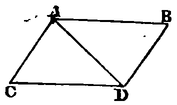
\includegraphics[width= 0.7\linewidth]{Fig/177px-Principia1846-084.png}
\caption{Figura utilizada por Newton para explicar a composição da ação das forças.\label{Fig:ComposicaoForcasNewton}}
\end{marginfigure}

De uma maneira mais direta, podemos dizer que a aceleração sofrida por um corpo sujeito a um conjunto de forças é dada pela soma vetorial das acelerações individuais que as forças -- agindo sozinhas, uma de cada vez -- imprimem sobre o corpo. O que, por sua vez, define uma força resultante que é dada pela soma das duas forças. Ou seja, existe uma força resultante $F_R$ tal que
\begin{align}
    \vec{F}_R &= \vec{F}_1 + \vec{F}_2 + \dots \\
    &= \sum_{i = 1}^n \vec{F}_i
\end{align}
%
e
\begin{equation}
    \vec{a} \propto \vec{F}_R.
\end{equation}

%%%%%%%%%%%%%%%%%%%%%%%%%%%%%%%%%%%%%%%%%%%%%
\subsection{Relação entre massa e aceleração}
%%%%%%%%%%%%%%%%%%%%%%%%%%%%%%%%%%%%%%%%%%%%%

Se aplicarmos uma força resultante em um corpo, temos que ele estará sujeito a uma aceleração. No entanto, se aplicarmos uma dada força em um corpo muito massivo, teremos uma aceleração pequena, ao passo que se aplicarmos tal força em um corpo com uma massa pequena, teremos uma aceleração maior. Percebemos então que a aceleração assume uma proporcionalidade inversa em relação à massa:
\begin{equation}
  a \propto \frac{1}{m},
\end{equation}
%
ou, considerando a dependência em relação à força e o caráter vetorial das grandezas,
\begin{equation}
  \vec{a} \propto \frac{\vec{F}_R}{m}.
\end{equation}
%
Considerando que a aceleração só dependa de $F$ e $m$, e também o fato de que uma proporcionalidade pode ser escrita como uma igualdade se utilizarmos uma constante de proporcionalidade $C$ qualquer -- cujo valor precisamos determinar -- temos
\begin{equation}
  \vec{a} = C \frac{\vec{F}_R}{m}.
\end{equation}

Apesar de termos unidades para a aceleração e para a massa, não temos para a força. Nesse caso, podemos englobar a constante $C$ na própria definição das unidades da força e obter
\begin{equation}\label{Eq:SegundaLeiDeNewton}
  \vec{a} = \frac{\vec{F}_R}{m} \mathnote{Segunda Lei de Newton.}
\end{equation}

A forma acima não é a mais conhecida, mas sim 
\begin{equation}
  \vec{F}_R = m \vec{a}.
\end{equation}
%
Matematicamente, as expressões são completamente equivalentes, porém a Equação~\ref{Eq:SegundaLeiDeNewton} deixa mais evidente a relação causa e efeito: \emph{a existência de uma força resultante causa uma aceleração}.\footnote{A inversão dessa causa e efeito é particularmente problemática ao tratarmos de forças no movimento circular, onde um erro comum é achar que existe uma força \emph{adicional} em movimentos circulares, denominada como \emph{força centrípeta}. Na verdade, alguma força, ou componente de força, exerce o papel de força centrípeta e \emph{causa} o movimento circular. Discutiremos isso em detalhes adiante.}

%%%%%%%%%%%%%%%%%%%%%%%%%%%%%%%
\subsection{Unidades e medidas}
%%%%%%%%%%%%%%%%%%%%%%%%%%%%%%%

Através da Segunda Lei de Newton, podemos determinar a massa de um objeto em relação à massa de outro. Suponha que tomamos um objeto qualquer e a ele aplicamos uma força resultante $F$. Sabemos que ele será submetido a uma aceleração de tal maneira que
\begin{equation}
  F = m_1 a_1.
\end{equation}
%
Se submetermos outro corpo à mesma força, temos
\begin{equation}
  F = m_2 a_2.
\end{equation}
%
Como a força é a mesma em ambos os casos, podemos escrever
\begin{equation}
  m_1 a_1 = m_2 a_2,
\end{equation}
%
ou
\begin{equation}
  m_2 = \frac{a_1}{a_2}m_1.
\end{equation}

Este resultado é relevante pois não temos um método de determinar a massa de um objeto a não ser por comparação com outro. No Sistema Internacional (SI), utiliza-se a massa de um cilindro metálico como massa padrão em relação a qual as demais massas são medidas, sendo atribuída a ele a massa de \np[kg]{1}. Utilizando o processo acima, podemos determinar a massa de um objeto qualquer em relação ao padrão de referência.

As medidas de força podem ser feitas através de uma mola. Veremos adiante que a força exercida por uma mola é proporcional à distensão que ela sofre. Assim, é possível elaborar um equipamento simples --~um dinamômetro~-- que consiste em uma mola associada a uma escala graduada. Dentro so SI, as unidades de força são
\begin{align}
    [F] &= [m a] \\
    &= [m] [a] \\
    &= \rm{kg} \frac{\rm{m}}{\rm{s}^2} \\
    &\equiv \rm{N},
\end{align}
%
onde utilizamos a definição $N \equiv \rm{kg}\cdot\rm{m}/\rm{s}^2$ para nomear a unidade da força como \emph{Newton}, isto é, $\np[N]{1} \equiv \np[kg\cdot m/s^2]{1}$.

%%%%%%%%%%%%%%%%%%%%%%%%%%%%%%%%
\section{Terceira Lei de Newton}
%%%%%%%%%%%%%%%%%%%%%%%%%%%%%%%%

A Terceira Lei de Newton foi por ele enunciada como
\begin{quote}
    Para cada ação há sempre uma reação igual oposta: ou as ações mutuas de dois corpos um sobre o outro são sempre iguais, e dirigidas a partes contrárias.
\end{quote}

\begin{marginfigure}
\centering
\begin{tikzpicture}[>=Stealth,
     interface/.style={
        % superfície
        postaction={draw,decorate,decoration={border,angle=-45,
                    amplitude=0.2cm,segment length=2mm}}},
    ]
    
    \draw[interface](-2,0) -- (2,0);
    
    \draw[pattern = north west lines, pattern color = gray] (-1,0) rectangle (0,1);
    \draw[pattern = north east lines, pattern color = gray] (0,1) rectangle (1,0);
    
    \draw[->] (-2, 0.5) -- node[above]{$\vec{F}$} +(1,0);
    \draw[->] (0,0.5) -- node [above]{$\vec{F}_{12}$} +(0.5,0);
    \draw[->] (0,0.5) -- node [above]{$\vec{F}_{21}$} +(-0.5,0);
    
    \draw[->] (-0.5,1.25) -- node[above]{$\vec{a}$} +(1,0);
\end{tikzpicture}
\caption{Ao submetermos dois blocos a uma força $\vec{F}$, ocorrerá uma interação na superfície de contato entre eles. Tal interação resultará na força $\vec{F}_{12}$ para a direita atuando no bloco da direita, fazendo com que ele acelere, e na força $\vec{F}_{21}$ para a esquerda atuando no bloco da esquerda. No caso do bloco da esquerda a \emph{força resultante} $\vec{F} - \vec{F}_{21}$ será a responsável pela aceleração.}
\end{marginfigure}

\noindent{}Denominamos tal par como um \emph{par ação--reação}. Note que as forças do par nunca atuam sobre o mesmo corpo: em uma interação entre dois corpos quaisquer, uma delas, $\vec{F}$, atua sobre um dos corpos, enquanto a outra\footnote{Sempre que tivermos um par ação--reação, denotaremos uma das forças usando a ``linha'', de forma a diferenciá-las.}, $\vec{F}'$, atua sobre o outro. Além disso, as forças têm o mesmo módulo. Finalmente, Newton contempla a interação por quaisquer meios, seja por contato, seja à distância.

\begin{marginfigure}
\centering
\begin{tikzpicture}[>=Stealth,
     interface/.style={
        % superfície
        postaction={draw,decorate,decoration={border,angle=-45,
                    amplitude=0.2cm,segment length=2mm}}},
    ]
    
    \draw[interface] (-2.5,0) -- (2.5,0);
    
    \draw (-2, 0) rectangle node[rotate=90]{N} (-1.5,0.5);
    \draw[fill] (-1.5,0.5) rectangle (-1,0);
    
    \draw (1, 0) rectangle node[rotate=90]{N} (1.5,0.5);
    \draw[fill] (1.5,0.5) rectangle (2,0);
    
    \draw[->] (-1,0.25) -- node[above]{$\vec{F}_{12}$} +(0.75,0);
    \draw[->] (1,0.25) -- node[above]{$\vec{F}_{21}$} +(-0.75,0);
    
    \draw[->] (-1.75,0.75) -- node[above]{$\vec{a}$} +(+0.5,0);
    \draw[->] (1.75,0.75) -- node[above]{$\vec{a}$} +(-0.5,0);
\end{tikzpicture}
\caption{Mesmo no caso de uma interação à distância, temos um par ação-reação: Na situação mostrada na figura, ambos os imãs se deslocariam na ausência de atrito estando sujeitos a uma aceleração $a = F_{12}/m_1 = F_{21}/{m_2}$.}
\end{marginfigure}

Muitas vezes, devido às diferentes massas dos corpos que interagem, pode ser difícil perceber que um deles está sujeito a uma força quando interage com outro. Se, por exemplo, um patinador arremessa uma bola com força, verificamos que a bola sofre uma grande alteração de sua velocidade. O patinador, por sua vez, sofre uma aceleração no sentido contrário -- no entanto, observamos que sua velocidade final é muito menor --. Isto pode ser entendido através da Segunda Lei de Newton, pois, como as forças que atuam  em cada um dos corpos são iguais em módulo
\begin{align}
  F &= m_1 a_1 \\
  F' &= m_2 a_2
\end{align}
%
e, consequentemente,
\begin{equation}
  a_2 = \frac{m_1}{m_2} a_1.
\end{equation}
%
Logo, se supomos que a massa $m_1$ da bola é muito menor que a massa $m_2$ do patinador, temos que $m_1/m_2 \ll 1$ e, consequentemente, $a_2 \ll a_1$. Como ambos os corpos estão sujeitos às acelerações durante o mesmo intervalo de tempo, observamos que $v_2 \ll v_1$, pois a velocidade é diretamente proporcional à duração da aceleração.

%%%%%%%%%%%%%%%%
\section{Forças}
%%%%%%%%%%%%%%%%

Através das Leis de Newton, fica evidente que transferimos o problema da determinação do movimento dos corpos para a determinação das forças que atuam sobre eles. Infelizmente, não existe uma lei que determine quais são as forças que atuam sobre um corpo, restando como única saída uma análise cuidadosa do fenômeno estudado.

A partir de experimentos, se tem o conhecimento de um pequeno número de forças que podem ser consideradas \emph{fundamentais}:
\begin{itemize}
  \item força gravitacional;
  \item força eletromagnética;
  \item força nuclear forte;
  \item força nuclear fraca.
\end{itemize}
%
Tais forças são denominadas fundamentais pois todas as demais podem ser interpretadas através delas. Em geral, no entanto, a descrição de fenômenos através delas não é prática. Do ponto de vista macroscópico, é mais útil trabalharmos com forças que surgem a partir de interações complexas dos átomos através das forças fundamentais.

Na lista acima, as duas primeiras são responsáveis pelas forças que estudaremos em mecânica, como a força peso (oriunda da força gravitacional) e as forças normal, de tensão, atrito, arrasto e elástica (oriundas da força eletromagnética). Outras expressões podem ser encontradas para outras situações, no entanto não as estudaremos a fundo aqui, como por exemplo as forças que atuam sobre cargas elétricas, entre condutores portando corrente, entre moléculas (força de van der Waals), etc. Em alguns casos, vamos tratar de forças de contato que tem origem eletromagnética, porém que não nos damos ao trabalho de nomear, como as forças que atuam entre duas esferas que colidem.

%%%%%%%%%%%%%%%%%%%%%%%%%%%%%%%%%%%%%%%%%%%%%%%%%%%%%%%%%%%%%%%%%%s
\subsection{Determinação de força resultante e diagramas de forças} 
%%%%%%%%%%%%%%%%%%%%%%%%%%%%%%%%%%%%%%%%%%%%%%%%%%%%%%%%%%%%%%%%%%s

Quando mais que uma força atua sobre um corpo, devemos determinar a \emph{força resultante} que atua sobre ele para que possamos determinar qual será a aceleração a qual ele estará submetido. Isso pode ser feito de maneira relativamente simples, bastanto utilizar as propriedades vetoriais. Assim,
\begin{equation}
    \vec{F}_R = \vec{F}_1 + \vec{F}_2 + \vec{F}_3 + \dots,
\end{equation}
%
onde tal soma deve ser feita observando as regras para a soma de vetores.

Como já vimos, tal processo pode ser facilitado se utilizarmos um \emph{sistema de coordenadas} no qual podemos decompor os vetores. A escolha do sistema de coordenadas é muito importante, pois um sistema inadequado pode dificultar muito a solução de um problema. Devemos observar os seguintes pontos:
\begin{itemize}
    \item Como regra geral, se houver aceleração no sistema, devemos escolher um dos eixos na direção de tal aceleração, pois assim teremos aceleração nula nos demais eixos.
    \item Caso não haja nenhuma aceleração, devemos verificar informações dadas sobre ângulos e procurar estabelecer eixos de forma que os ângulos entre as forças e os eixos sejam conhecidos.
    \item Finalmente, devemos procurar eixos que minimizem o número de forças que devem ser decompostas.
\end{itemize}
%
Uma vez escolhido um sistema de coordenadas, devemos aplicar a Segunda Lei de Newton a cada um deles separadamente, uma vez para cada eixo de referência de cada corpo. A partir das equações obtidas, devemos buscar as informações que necessitamos. Muitas vezes vamos precisar elaborar sistemas de equações para que possamos determinar tais informações.

\begin{marginfigure}
\centering
\begin{tikzpicture}[>=Stealth,
     interface/.style={
        % superfície
        postaction={draw,decorate,decoration={border,angle=-45,
                    amplitude=0.2cm,segment length=2mm}}},
    ]
    
    \draw[interface] (-1,0) -- (1,0);
    
    \draw[pattern= north west lines] (-0.5,0) rectangle (0.5,1);
    \draw[fill] (0,0.5) circle (1pt);
    
    \draw[dashed,->] (-1, 0.5) -- (1, 0.5) node[above left]{$x$};
    \draw[dashed,->] (0,-1) -- (0,2.5) node[below right]{$y$};
    
    \draw[->, thick] (0, 0.5) -- (0,-0.5) node[left]{$\vec{P}$};
    \draw[->, thick] (0,1) -- (0,2) node[left]{$\vec{N}$};
    
    \draw[fill] (2,0.5) circle (1pt);
    \draw[->, thick] (2,0.5) -- +(0,1) node[right]{$\vec{N}$};
    \draw[->, thick] (2,0.5) -- +(0,-1) node[right]{$\vec{P}$};
    
    \draw[dashed, ->](1.5,0.5) -- (2.5, 0.5) node[above left]{$x$};
    \draw[dashed, ->](2,-1) -- (2,2.5) node[below right]{$y$};
    
\end{tikzpicture}
\caption{Esboço de um problema e o diagrama de forças do problema. Apesar de a rigor devermos utilizar o diagrama, é mais ilustrativo utilizar a representação da esquerda, porém ela tem problemas conceituais: a força $\vec{N}$ exercida pela mesa é exercida na parte inferior do bloco, não no topo, como ilustrado.\label{Fig:DiagramaDeForcasEEsboco}}
\end{marginfigure}

Um artifício fundamental para a interpretação e solução de problemas de dinâmica é o \emph{diagrama de corpo livre}, ou \emph{diagrama de forças}. Tal diagrama consiste em um ponto que representa um corpo, sendo que todas as forças que atuam sobre tal corpo são representadas como atuando sobre um ponto, que representa o centro de massa do corpo (veja a parte à direita na Figura~\ref{Fig:DiagramaDeForcasEEsboco}). Além disso, não devemos incluir acelerações, velocidades, ou quaisquer outros vetores no diagrama de forças.

Podemos, ao invés de utilizar um diagrama de forças como descrito acima, fazer um esboço da situação (veja a parte à esquerda na Figura~\ref{Fig:DiagramaDeForcasEEsboco}). Isso em geral é mais interessante, pois ele reúne as principais características de um diagrama de forças e ao mesmo tempo permite uma visualização do problema. Esse artifício exige algumas adaptações, como representar forças em posições diferentes das ideais para que elas possam ser representadas confortavelmente no esboço.

%%%%%%%%%%%%%%%%%%%%%%%%%%%%%%%%%
\paragraph{Equilíbrio de forças}
%%%%%%%%%%%%%%%%%%%%%%%%%%%%%%%%%

\begin{marginfigure}[3cm]
\centering
\begin{tikzpicture}[>=Stealth]
    \draw[pattern = north west lines] (0,0) rectangle (1,1);
    
    \draw[->, thick] (1,1) coordinate (BL) -- +(1,1) coordinate (F) node[right]{$\vec{F}_1$};
    \draw[->, thick] (0.5,0) -- +(0,-1) node[right]{$\vec{F}_2$};
    \draw[->, thick] (0,0.5) -- +(-1,0) node[above]{$\vec{F}_3$};
    
    \draw[dashed] (1,1) -- +(1,0) coordinate (X);
    
    \pic[draw, "$\theta$", angle eccentricity = 1.5]{angle = X--BL--F};
\end{tikzpicture}
\caption{Um corpo submetido a um conjunto de forças e em equilíbrio.\label{Fig:ExemploEquilibrio}}
\end{marginfigure}

Uma situação particularmente comum é quando a força resultante sobre um corpo é nula. Nesse caso, temos o que chamamos de uma \emph{situação de equilíbrio}. Através da Segunda Lei de Newton, verificamos que a aceleração do corpo nessa situação é zero. Note que o equilíbrio não significa que a velocidade é necessariamente zero, pois uma velocidade constante satisfaz a condição de ``aceleração nula'' perfeitamente.

Na Figura~\ref{Fig:ExemploEquilibrio} temos um corpo sujeito a um conjunto de forças e em equilíbrio. Podemos determinar a relação entre as forças através da Segunda Lei de Newton. Para isso, vamos adotar um sistema de referência e determinar o ângulo entre as forças e os eixos. Veja a Figura~\ref{Fig:ExemploEquilibrioRef}. Aplicando a Segunda Lei de Newton a cada eixo, temos:
\begin{description}
    \item[Eixo $x$:]
        \begin{align}
            F_R^x &= m a_x \\
            F_1^x - F_3 &= 0 \\
            F_1^x &= F_3.
        \end{align}
    \item[Eixo $y$:]
        \begin{align}
            F_R^y &= m a_y \\
            F_1^y - F_2 &= 0 \\
            F_1^y &= F_2.
        \end{align}
\end{description}

\begin{marginfigure}[-5cm]
\centering
\begin{tikzpicture}[>=Stealth]
    \draw[pattern = north west lines] (0,0) rectangle (1,1);
    
    \draw[->, thick] (1,1) coordinate (BL) -- +(1,1) coordinate (F1) node[right]{$\vec{F}_1$};
    \draw[->, thick] (0.5,0) -- +(0,-1) node[right]{$\vec{F}_2$};
    \draw[->, thick] (0,0.5) -- +(-1,0) node[above]{$\vec{F}_3$};
    
    \draw[->, dashed] (-1.5,0.5) -- (2.5,0.5) node[below left]{$x$};
    \draw[->, dashed] (0.5, -1.5) -- (0.5, 2) node[below left]{$y$};
    
    \draw[dashed] (1,1) -- +(1,0) coordinate (X);
    \pic[draw, "$\theta$", angle eccentricity = 1.5] {angle = X--BL--F1};
\end{tikzpicture}
\caption{Um corpo submetido a um conjunto de forças e em equilíbrio.\label{Fig:ExemploEquilibrioRef}}
\end{marginfigure}

\noindent{}Em ambos os eixos utilizamos o fato de que, se há equilíbrio no eixo, então a aceleração é nula. A força $\vec{F}_1$ pode ser decomposta utilizando as funções trigonométricas e o fato de que o ângulo entre a força e o eixo $x$ será $\theta$, o que resulta em
\begin{align}
    F_1 \cos\theta &= F_3 \\
    F_2 \sen\theta &= F_2.
\end{align}

Note que a escolha do sistema de referências foi feita com base no ângulo dado e no fato de que as forças $\vec{F}_2$ e $\vec{F}_3$ não precisariam ser decompostas. No entanto, outros sistemas poderiam ser utilizados, desde que conseguíssemos determinar o ângulo entre cada força e os eixos de referência.

%%%%%%%%%%%%%%%%%%%%%%%%%%%%%%%%%%%%%%%%%%%%%
\subsection{Força gravitacional e força peso} 
%%%%%%%%%%%%%%%%%%%%%%%%%%%%%%%%%%%%%%%%%%%%%

Sabemos que próximo da superfície da Terra, todos os corpos estão sujeitos a uma aceleração de aproximadamente \np[m/s^2]{9,8} (ignorando-se os efeitos da resistência do ar). A origem dessa aceleração e sua independência em relação à massa podem ser explicadas através da Teoria da Gravitação Universal, também proposta por Newton. Segundo ela, dois corpos quaisquer está sujeitos a uma força de atração mútua -- isto é, atuando sobre ambos os corpos, constituindo um par ação-reação -- dada por

\begin{marginfigure}
\centering
\begin{tikzpicture}[>=Stealth]

    \draw[dotted] ([shift={(0,0)}]180:2) arc[radius=2, start angle=180, end angle= 0];
    \draw[fill] (0,0) circle (1pt) node[left]{$C$};
    \draw[->, thick] (0,0) -- node[right]{$\vec{P}'$} +(0,1);
    
    \draw[pattern= north west lines] (0,3.5) circle (3mm);
    \draw[fill] (0,3.5) circle (1pt);
    \draw[->, thick] (0,3.5) -- node[right]{$\vec{P}$} +(0,-1);
\end{tikzpicture}
\caption{Par ação-reação para a força peso: a interação gravitacional se dá entre o planeta e o objeto, logo temos uma reação que atua na Terra. Como tratamos corpos rígidos como pontos, podemos representar a reação como uma força que atua no centro de massa do planeta.}
\end{marginfigure}

\begin{equation}\label{Eq:LeiGravitacaoUniversal}
  F_g = G \frac{m_1 m_2}{r^2}.
\end{equation}

\noindent{}Nesta expressão, $G$ representa uma constante universal cujo valor é de \np[N\cdot m^2/kg^2]{6.6725985e-11}, $m_1$ e $m_2$ representam as massas dos corpos que interagem, e $r$ representa a distância de separação entre os dois corpos.

Aplicando a expressão acima para o caso de um corpo de massa $m$ nas imediações da superfície da Terra, temos
\begin{equation}
  F_g = \left[G \frac{m_T}{r_T^2}\right]m,
\end{equation}
%
onde $m_T$ e $r_T$ representam a massa e o raio da Terra, respectivamente. Utilizamos o raio da Terra pois consideramos que toda a massa está contida no centro de massa. Se aproximarmos a Terra como uma esfera homogênea, tal ponto dista da superfície pelo raio da esfera. Um corpo sujeito a tal força terá então uma aceleração dada por
\begin{equation}
  F_g = ma
\end{equation}
%
ou,
\begin{equation}\label{Eq:EliminaM}
  ma = m \left[G \frac{m_T}{r_T^2}\right].
\end{equation}
%
Dividindo ambos os lados da equação por $m$, temos que a aceleração será dada por
\begin{equation}
  a = \left[G \frac{m_T}{r_T^2}\right] \approx \np[m/s^2]{9,8}.
\end{equation}
%
Portanto, o valor $g$ a que nos referimos ao estudar a queda livre é dado pela equação acima, isto é,
\begin{equation}
  g = \left[G \frac{m_T}{r_T^2}\right].
\end{equation}

%%%%%%%%%%%%%%%%%%%%%%%%%%%%%%%%%%%%%%%%%%%%
\paragraph{Aceleração em um plano inclinado}
%%%%%%%%%%%%%%%%%%%%%%%%%%%%%%%%%%%%%%%%%%%%

Em um plano inclinado, a aceleração depende do ângulo entre o plano e a horizontal. Se o ângulo é zero, temos uma situação em que não há aceleração alguma; se o ângulo for de \np[\tcdegree]{90}, temos a própria aceleração da gravidade.

\begin{marginfigure}
\centering
\begin{tikzpicture}[>=Stealth, rotate=-35,
     interface/.style={
        % superfície
        postaction={draw,decorate,decoration={border,angle=-45,
                    amplitude=0.2cm,segment length=2mm}}},
    ]
   
    \draw[dashed, ->] (0,0.5) -- (4,0.5) node[below left]{$x$};
    \draw[dashed, ->] (2,-1) -- (2,2.5) node[below right]{$y$};
    
    \draw[interface] (0,0) -- (4,0);
    \draw[pattern= dots] (1.5,0) rectangle (2.5,1);
        
    \draw[fill] (2,0.5) circle (1pt);
    \draw[->, thick] (2,0.5) -- +(-55:1) node[left]{$\vec{P}$};
    \draw[->, thick] (2,1) -- +(0,0.81915) node[below right]{$\vec{N}$};
    
    \draw[->] (3,1) -- node[above]{$\vec{a}$}(3.7,1);
    
    \coordinate (A) at (4,0);
    \draw[dashed] (A) -- +(-145:1) coordinate (B);
    \coordinate (O) at (0,0);
    
    \draw[dashed] (A) -- (B);
    \pic [draw, "$\theta$", angle eccentricity=1.5] {angle = O--A--B};

\end{tikzpicture}
\caption{Bloco sobre plano inclinado. Escolhemos o sistema de coordenadas de maneira que a aceleração esteja contida em apenas um dos eixos.\label{Fig:BlocoPlanoInclinadoAcel}}
\end{marginfigure}

Na Figura~\ref{Fig:BlocoPlanoInclinadoAcel} temos um esboço dessa situação. Escolhemos um sitema de referência de maneira que a aceleração esteja contida em somente um dos eixos, o eixo $x$. No eixo $y$ denotamos a força normal $\vec{N}$ exercida pela superfície sobre o bloco --~veremos mais detalhes sobre essa força na proxima seção~--. Também denotamos a força peso, porém verificamos que ela tem componentes tanto no eixo $x$ quanto no eixo $y$.

\begin{marginfigure}
\centering
\begin{tikzpicture}[>=Stealth, rotate=-35,
     interface/.style={
        % superfície
        postaction={draw,decorate,decoration={border,angle=-45,
                    amplitude=0.2cm,segment length=2mm}}},
    ]
     
    \draw[interface, gray] (0,0) -- (4,0);
    \draw[pattern= dots, pattern color = gray] (1.5,0) rectangle (2.5,1);
        
    \draw[fill, gray] (2,0.5) circle (1pt);
    \draw[->, thick, gray] (2,0.5) -- +(-55:1) node[left]{$\vec{P}$};
    \draw[->, thick, gray] (2,1) -- +(0,0.81915) node[below right]{$\vec{N}$};
       
    \path[name path = solo] (4,0)+(-145:3) -- +(35:1);
    \path[name path = eixop] (2,0.5) -- +(-55:1.75);
    \path[name path = eixox] (2,0.5) -- (5,0.5);
    \path[name path = eixoy] (2,0.5) -- +(0,-2);
    
    \draw[dashed, name intersections={of=solo and eixox}] (2,0.5) -- (intersection-1) coordinate (A);
    \draw[dashed, name intersections={of=solo and eixop}] (2,0.5) -- (intersection-1);
    \draw[dashed, name intersections={of=solo and eixoy}] (2,0.5) -- (intersection-1) coordinate (B);
    \draw[dashed] (A) -- (B);

    \coordinate (O) at (0,0.5);
    
    \pic [draw, "$\theta$", angle eccentricity=1.5] {angle = O--A--B};
    
    \coordinate (C) at (4,0);
    \coordinate (OS) at (0,0);
    \pic [draw, "$\theta$", angle eccentricity=1.5, gray] {angle = OS--C--B};
    
\end{tikzpicture}
\caption{Triângulo para a determinação do ângulo entre $\vec{P}$ e os eixos de referência.\label{Fig:TrianguloAnguloPesoPlanoInclinado}}
\end{marginfigure}

Para que possamos decompor a força peso, precisamos saber os ângulos entre tal força e os eixos de referência. Na Figura~\ref{Fig:TrianguloAnguloPesoPlanoInclinado} extendemos o eixo $x$ até que ele intercepte o eixo horizontal na base do plano inclinado. Como o eixo é paralelo ao plano, se o ângulo entre este e a horizontal é $\theta$, o ângulo entre o eixo $x$ e a horizontal também é $\theta$.

Vamos analisar o triângulo formado pelo eixo $x$, pelo eixo $y$, pela direção da força peso, e pela horizontal -- veja a Figura~\ref{Fig:TrianguloAnguloPesoPlanoInclinadoAngulos}. No triângulo da direita temos que
\begin{equation}
    \theta + \alpha + \np[\tcdegree]{90} = \np[\tcdegree]{180},
\end{equation}
%
onde usamos o fato de que a soma dos ângulos internos de um triângulo é sempre \np[\tcdegree]{180}. Também temos, verificando o canto superior do triângulo como um todo, que
\begin{equation}
    \alpha + \beta = \np[\tcdegree]{90}.
\end{equation}
%
\begin{marginfigure}
\centering
\begin{tikzpicture}[>=Stealth, rotate=-35,
     interface/.style={
        % superfície
        postaction={draw,decorate,decoration={border,angle=-45,
                    amplitude=0.2cm,segment length=2mm}}},
    ]
           
    \path[name path = solo] (4,0)+(-145:3) -- +(35:1);
    \path[name path = eixop] (2,0.5) -- +(-55:1.75);
    \path[name path = eixox] (2,0.5) -- (5,0.5);
    \path[name path = eixoy] (2,0.5) -- +(0,-2);
    
    \draw[name intersections={of=solo and eixox}] (2,0.5) -- (intersection-1) coordinate (A);
    \draw[name intersections={of=solo and eixop}] (2,0.5) -- (intersection-1) coordinate (P);
    \draw[name intersections={of=solo and eixoy}] (2,0.5) -- (intersection-1) coordinate (B);
    \draw (A) -- (B);

    \coordinate (O) at (2,0.5);
    
    \pic [draw, "$\theta$", angle eccentricity=1.5] {angle = O--A--B};
    \pic [draw, "$\beta$", angle eccentricity=1.5, angle radius = 5.5 mm] {angle = B--O--P};
    
    \pic [draw, "$\alpha$", angle eccentricity=1.5, angle radius = 4.5 mm] {angle = P--O--A};
    
    \pic [draw, "$\cdot$", angle eccentricity=0.5, angle radius = 3mm] {angle = A--P--O};
    \pic [draw, "$\cdot$", angle eccentricity=0.5, angle radius = 3mm] {angle = B--O--A};
    \pic [draw, "$\cdot$", angle eccentricity=0.5, angle radius = 3mm] {angle = O--P--B};
        
\end{tikzpicture}
\caption{Triângulos formados pelos eixos $x$, $y$, pela direção de $\vec{P}$, e pela horizontal. \label{Fig:TrianguloAnguloPesoPlanoInclinadoAngulos}}
\end{marginfigure}
Isolando $\alpha$ na equação acima obtemos
\begin{equation}
    \alpha = \np[\tcdegree]{90} - \beta
\end{equation}
%
que podemos substituir na equação obtida para o triângulo da direita, o que resulta em
\begin{align}
        \theta + \np[\tcdegree]{90} - \beta + \np[\tcdegree]{90} &= \np[\tcdegree]{180} \\
        \theta - \beta &= 0 \\
        \theta &= \beta.
\end{align}
%
Concluímos então que o ângulo entre o eixo perpendicular ao plano e a direção da força peso é igual ao ângulo entre o plano e a horizontal. Esse resultado será fundamental para avaliarmos todas as situações envolvendo planos inclinados.

Agora podemos aplicar a Segunda Lei de Newton para os dois eixos
\begin{description}
    \item[Eixo $x$:] No eixo paralelo ao plano temos
        \begin{align}
            F_R^x &= m a_x \\
            P_x &= m a_x \\
            P \sen\theta &= m a_x \\
            mg \sen\theta &= ma_x,\label{Eq:AceleracaoPlanoInclinadoM}
        \end{align}
    \item[Eixo $y$:] No eixo perpendicular ao plano temos
        \begin{align}
            F_R^y &= m a_y \\
            N - P_y &= 0 \\
            N &= P \cos\theta \\
            N &= mg \cos\theta,
        \end{align}
\end{description}
%
Nas equações acima, utilizamos o fato de que não há aceleração no eixo perpendicular ao plano para escrever o termo à direita da igualdade no segundo passo. Além disso, utilizamos as funções trigonométricas para determinar as componentes da força peso.

Finalmente, ao dividirmos ambos os lados da Equação~\ref{Eq:AceleracaoPlanoInclinadoM} pela massa, obtemos
\begin{equation}
    a_x = g \sen\theta.
\end{equation}
%
Verificamos, portanto, que a aceleração em um plano inclinado varia conforme alteramos a inclinação deste em relação à horizontal.

%%%%%%%%%%%%%%%%%%%%%%%%%
\subsection{Força Normal} 
%%%%%%%%%%%%%%%%%%%%%%%%%

Qualquer objeto próximo da Terra sofre uma atração em direção ao centro da Terra, mas nem todos são acelerados por tal força. Um objeto que repousa sobre o solo, por exemplo, se mantém parado, sem afundar no chão. Acontece que, nesse caso, as forças de origem eletromagnéticas de interação entre os átomos do solo e do objeto atuam de maneira a impedir que ele afunde. Isso, no entanto, não ocorre em todas as superfícies: se colocarmos um bloco de concreto sobre a água, por exemplo, ele afunda, indo em direção ao centro da Terra. No primeiro caso, denominamos a força resultante da interação entre os átomos da superfície e do bloco como \emph{força normal}. Ela recebe esse nome pois é sempre perpendicular à superfície e um vetor perpendicular a uma superfície é denominado em matemática como um vetor normal. No segundo caso, a interação eletromagnética não é suficiente para o manter em equilíbrio, porém ainda temos uma força resultante exercida pelos átomos, denominada de \emph{empuxo}.

\begin{marginfigure}[-4cm]
\centering
\begin{tikzpicture}[>=Stealth,
     interface/.style={
        % superfície
        postaction={draw,decorate,decoration={border,angle=-45,
                    amplitude=0.2cm,segment length=2mm}}},
    ]
    
    \draw[interface, gray] (-1,0) -- (1,0);
    
    \draw[pattern = north west lines, pattern color = gray] (-0.5,0) rectangle (0.5,1);
    \draw[fill] (0,0.5) circle (1pt);
    
    \draw[->, thick] (0, 0.5) -- +(0,-1) node[right]{$\vec{P}$};
    \draw[->, thick] (0,1) -- +(0,1) node[left]{$\vec{N}$};
    
    \draw[->, thick] (-0.3,0) -- node[left]{$\vec{N}'$} +(0,-1);
\end{tikzpicture}
\caption{A força normal é resultado de uma interação entre a superfície e o corpo. A reação $\vec{N}'$ atua sobre a superfície, na mesma direção que $\vec{N}$, com a mesma intensidade, porém com sentido oposto.}
\end{marginfigure}

Se a força normal é o resultado da interação de um corpo com uma superfície, sendo que a primeira força atua sobre o corpo, temos que a reação atua sobre a superfície. Se, por exemplo, colocamos uma caixa sobre uma mesa e o sistema se mantém em equilíbrio, temos que a força normal está dirigida para cima, perpendicularmente à superfície de contato e equilibrando a caixa. Sobre a mesa, dirigida perpendicularmente à superfície, mas dirigida para a mesa, temos a reação da força normal. Outro exemplo que vale a pena citar é o de uma balança de farmácia: quando subimos nela, e permanecemos imóveis, temos que a normal exercida pela balança equilibra nosso peso.  Devido ao fato de que nenhum dispositivo consegue verificar o valor de uma grandeza que não atue sobre ele, temos que a balança deve verificar o valor da reação à força normal, já que tal reação atua sobre a balança. O fato de termos que ficar parados para evitar a mudança da leitura da balança já nos dá um indício de que os valores indicados não se referem ao peso, pois $P = mg$ -- considerando que $m$ e $g$ são constantes durante a medida -- e é constante.

\begin{marginfigure}
\centering
\begin{tikzpicture}[>=Stealth,
     interface/.style={
        % superfície
        postaction={draw,decorate,decoration={border,angle=-45,
                    amplitude=0.2cm,segment length=2mm}}},
    ]
    
    \draw[interface, gray] (0,-1) -- (0,1);
    
    \draw[pattern = north west lines, pattern color = gray] (0,-0.5) rectangle (-1,0.5);
    \draw[fill] (-0.5,0) circle (1pt);
    
    \draw[->, thick] (-0.5, 0) -- +(0,-1) node[right]{$\vec{P}$};
    \draw[->, thick] (-1,0) -- +(-1,0) node[above]{$\vec{N}$};
    
    \draw[<-, thick] (-1,-0.5) -- node[below]{$\vec{F}$} +(-135:1.41421);
\end{tikzpicture}
\caption{No caso de contato com uma superfície vertical, temos uma força normal horizontal.}
\end{marginfigure}

Finalmente, devemos indicar que a força normal não pode ser encontrada por outra maneira além de resolver a Segunda Lei de Newton. Se desejamos saber o valor do peso de um objeto, podemos calculá-lo sabendo a massa e da aceleração da gravidade. Já para a força normal, não existe uma expressão que a relacione a outras grandezas, exceto pela própria Segunda Lei. Podemos afirmar de maneira simplificada que a força normal cresce de modo a equilibrar outras forças que atuam perpendicularmente em direção à superfície, porém limitando-se a um valor máximo de intensidade de força. Por exemplo, quando colocamos uma caixa leve sobre uma mesa frágil, verificamos que o sistema permanece em equilíbrio. Se passamos a depositar objetos no interior da caixa, verificamos que a força normal exercida pela mesa sobre a caixa deve aumentar progressivamente, mantendo o sistema em equilíbrio. Eventualmente, a caixa se tornará muito pesada e -- lembrando-se de que existe uma reação à força normal e que esta reação atua sobre a mesa -- excederemos o valor máximo de força tolerado pela mesa, que acaba se quebrando.

%%%%%%%%%%%%%%%%%%%%%%%%%%%%%%%%%%%%%%%%%%%%%%%%%%%%%%%%%%%%%
\paragraph{Força normal em sistemas submetidos a acelerações}
%%%%%%%%%%%%%%%%%%%%%%%%%%%%%%%%%%%%%%%%%%%%%%%%%%%%%%%%%%%%%

Se um objeto está disposto sobre o piso de um elevador e este passa a acelerar, a combinação entre as ações da força normal e da força peso é responsável por tal aceleração. Como o peso é constante, pois depende somente da massa do objeto e da aceleração da gravidade no local -- ambas constantes --, verificamos que \emph{o módulo da força normal varia de acordo com a aceleração} (veja a Figura~\ref{Fig:NormalVariaComAceleracao}).

\begin{figure}[!h]
\centering
\begin{tikzpicture}[>=Stealth,
     interface/.style={
        % superfície
        postaction={draw,decorate,decoration={border,angle=-45,
                    amplitude=0.2cm,segment length=2mm}}},
    ]
    
    \draw[interface] (-1,0) -- (1,0);
    
    \draw[pattern= north west lines] (-0.5,0) rectangle (0.5,1);
    \draw[fill] (0,0.5) circle (1pt);
    
    \draw[->, thick] (0, 0.5) -- +(0,-1) node[left]{$\vec{P}$};
    \draw[->, thick] (0,1) -- +(0,1.5) node[left]{$\vec{N}$};
    
    \draw[->] (0.7, 0.5) -- node[right]{$\vec{a}$} +(0,1);
    
    %
    
    \draw[interface] (2,0) -- (4,0);
    
    \draw[pattern= north west lines] (2.5,0) rectangle (3.5,1);
    \draw[fill] (3,0.5) circle (1pt);
    
    \draw[->, thick] (3, 0.5) -- +(0,-1) node[left]{$\vec{P}$};
    \draw[->, thick] (3,1) -- +(0,0.5) node[left]{$\vec{N}$};
    
    \draw[->] (3.7, 1.5) -- node[right]{$\vec{a}$} +(0,-1);
        
    %
    
    \draw[interface] (5,0) -- (7,0);
    
    \draw[pattern= north west lines] (5.5,0) rectangle (6.5,1);
    \draw[fill] (6,0.5) circle (1pt);
    
    \draw[->, thick] (6, 0.5) -- +(0,-1) node[left]{$\vec{P}$};
    \draw[->, thick] (6,1) -- +(0,1) node[left]{$\vec{N}$};
    
    \node (A) at (7.1, 0.5) {$\vec{a} = 0$};
\end{tikzpicture}
\caption{O valor da normal depende da aceleração do sistema.\label{Fig:NormalVariaComAceleracao}}
\end{figure}

Vamos tomar a primeira situação na Figura~\ref{Fig:NormalVariaComAceleracao} e definir um sistema de referência de forma que o eixo $y$ seja na direção e sentido da aceleração. Analisando o movimento nos eixos $x$ e $y$, temos
\begin{marginfigure}[5cm]
\centering
\begin{tikzpicture}[>=Stealth,
     interface/.style={
        % superfície
        postaction={draw,decorate,decoration={border,angle=-45,
                    amplitude=0.2cm,segment length=2mm}}},
    ]
    
    \draw[interface] (-1,0) -- (1,0);
    
    \draw[pattern= north west lines] (-0.5,0) rectangle (0.5,1);
    \draw[fill] (0,0.5) circle (1pt);
    
    \draw[->, thick] (0, 0.5) -- +(0,-1) node[left]{$\vec{P}$};
    \draw[->, thick] (0,1) -- +(0,1.5) node[left]{$\vec{N}$};
    
    \draw[->, gray] (0.7, 0.8) -- node[right]{$\vec{a}$} +(0,1);
    
    \draw[->, dashed] (-1,0.5) -- (1,0.5) node[below left]{$x$};
    \draw[->, dashed] (0, -1) -- (0,3.5) node[below left]{$y$};
\end{tikzpicture}
\end{marginfigure}

\begin{description}
    \item[Eixo $x$:] Não há forças aplicadas na direção deste eixo.
    \item[Eixo $y$:]
        \begin{align}
            F_R^y &= m a_y \\
            N - P &= m a_y \\
            N &= P + m a_y \\
            N &= mg + m a_y \\
            N &= m(g + a_y). \label{Eq:NormalComAceleracao}
        \end{align}
\end{description}

\noindent{}Note que quanto maior for o módulo da aceleração -- que assumimos como sendo no sentido positivo do eixo $y$ --, maior será o valor da força normal. Além disso, se tivermos uma aceleração nula, o que corresponde ao caso de o bloco estar simplesmente repousando sobre a superfície do chão do elevador, temos que a normal será igual ao peso:
\begin{equation}
    N = mg.
\end{equation}
%
Este resultado só é válido se a \emph{aceleração vertical for nula}.

Sempre que escrevemos a Segunda Lei de Newton para um eixo $i$ qualquer, utilizamos a expressão
\begin{equation}
    F_R^i = m a_i,
\end{equation}
%
e assumimos que a aceleração seja positiva --~ou seja, na direção positiva do eixo~--. Se estamos interessados em calcular a aceleração, podemos ter três tipos de resultados:
\begin{description}
    \item[Zero:] O sistema está em equilíbrio;
    \item[Positivo:] A aceleração é no sentido positivo que escolhemos para o eixo;
    \item[Negativo:] A aceleração é no sentido negativo do eixo, isto é, está no \emph{sentido oposto} ao que presumimos (assumindo que escolhemos o eixo na direção e sentido da aceleração, ou melhor, do que imaginávemos que seria o sentido da aceleração).
\end{description}

No caso de estarmos interessados em calcular uma força, como é o nosso caso neste momento, podemos contemplar a possibilidade de a aceleração ser tanto no sentido positivo do eixo que escolhemos, quanto no sentido negativo. Se a aceleração for no sentido negativo, basta utilizarmos \emph{valores negativos}. Assim, no caso de haver uma aceleração para baixo, temos simplesmente que a aceleração na expressão~\eqref{Eq:NormalComAceleracao} será negativa. Em termos do módulo da aceleração, isso significa fazer a substituição $a_y \to -|a_y|$, ou seja\footnote{Veja que essa substituição pelo módulo não é necessária, basta utilizarmos valores de aceleração negativos na Equação~\ref{Eq:NormalComAceleracao}. Fizemos essa substiuição aqui só para tornar mais evidente o fato de que ao acelerarmos para baixo o valor da normal \emph{diminui}.}
\begin{equation}
    N = m(g - |a_y|).
\end{equation} 
%
Vemos da expressão acima que ao acelerarmos para baixo, o valor da normal \emph{diminui} com o aumento do módulo da aceleração.

%%%%%%%%%%%%%%%%%%%
\subsection{Tensão} 
%%%%%%%%%%%%%%%%%%%

Ao pendurarmos um objeto utilizando uma corda, se temos equilíbrio, existe uma \emph{tensão} exercida pela corda que equilibra a força peso do objeto. As forças de tensão também têm origem eletromagnética (se originam das interações eletromagnética entre os átomos que compõe as fibras da corda) e têm características parecidas com as da força normal: podemos determiná-las somente com mais detalhes da situação e temos um valor máximo de força, sendo que a corda se rompe ao excedê-lo\footnote{Na verdade a corda não se rompe repentinamente, suas fibras se partem e a corda estica, cedendo aos poucos e diminuindo (mesmo que momentaneamente) a tensão exercida. Eventualmente muitas fibras se rompem e dão início a uma ``reação em cadeia'' de rompimento das fibras. O valor máximo de força exercido certamente ocorre antes de esse processo ocorrer.}. Outra consideração importante é que uma corda só consegue exercer forças quando são esticadas, não exercendo -- portanto -- forças laterais ou no sentido de ``dobrá-la'' (no sentido contrário ao de esticá-la). 

Se a massa da corda não puder ser desprezada, não faz sentido falarmos em uma ``tensão na corda'': a tensão será diferente em cada ponto dela. Em especial, no ponto inferior, vemos que a tensão exercida deve sustentar somente o peso da caixa. No ponto superior, a tensão deve sustentar tanto o peso da caixa, como o da corda. Vemos, também que as tensões nos pontos superior e inferior não são pares ação-reação, pois tais tensões não tem o mesmo módulo. Na verdade, o par ação-reação ocorre nos pontos de interação entre dois corpos e, portanto, temos um par ação-reação para uma das extremidades e outro par ação-reação que atua na outra extremidade, em cada caso com uma força na corda e outra no objeto. Se a massa da corda for negligível\footnote{Se consideramos a corda como de massa desprezível, na prática estamos considerando que os dois corpos ao quais ela está amarrada interagem diretamente, o que não é verdade (apesar de ser o caso que vamos considerar aqui).}, é possível mostrar que as tensões superior e inferior terão o mesmo valor, porém continuarão não sendo um par ação-reação: em tal par, cada uma das forças atua em um dos corpos que interagem (corda-teto, ou corda-caixa), mas $\vec{T}'_s$ e $\vec{T}'_i$ atuam no teto e na caixa, que não interagem diretamente. Além disso, $\vec{T}_s$ e $\vec{T}_i$ atuam no mesmo corpo.

\begin{marginfigure}
\centering
\begin{tikzpicture}[>=Stealth,
     interface/.style={
        % superfície
        postaction={draw,decorate,decoration={border,angle=-45,
                    amplitude=0.2cm,segment length=2mm}}},
    ]
    \draw[interface, gray] (1,0) -- (-1,0);
    \draw[pattern = north west lines, pattern color = gray] (-0.05,0) rectangle (0.05,-3);
    
    \draw[->, thick] (0,0) -- node[right]{$\vec{T}'_s$} +(0,0.6);
    \draw[->, thick] (0,0) -- node[right]{$\vec{T}_s$} +(0,-0.6);
    
    \draw (-0.5, -3) rectangle (0.5, -4);
    \draw[->, thick] (0, -3) -- node[above right]{$\vec{T}_i$} +(0,0.4);
    \draw[->, thick] (0, -3) -- node[below right]{$\vec{T}'_i$} +(0, -0.4);
    
    \draw[fill, gray] (0, -3.5) circle (1pt);
    \draw[->, gray] (0, -3.5) -- +(0,-1) node[right]{$\vec{P}$};
\end{tikzpicture}
\caption{Se considerarmos uma corda real, onde a massa não pode ser negligenciada, temos que a tensão é diferente para cada ponto da corda.}
\end{marginfigure}

Outro caso em que a massa de uma corda é importante, é aquele em que ela fica disposta horizontalmente. Nesse caso, se tomarmos um segmento qualquer da corda, verificamos que para que ele se mantenha em equilíbrio, deve haver alguma força que equilibre a força peso do segmento. Tal força é a própria tensão na corda, que atua para ambos os lados do segmento, porém tem pequenas componentes dirigidas para cima e, dessa forma, se estabelece um equilíbrio. Cada segmento, no entanto está submetido a forças que fazem ângulos diferentes em relação à horizontal. Isso da origem a uma forma específica para a curva de posição vertical em função da posição horizontal, conhecida como \emph{catenária}, mostrada na Figura~\ref{Fig:Catenaria}. Essa forma corresponde àquela dos fios pendurados entre dois postes.

\begin{marginfigure}
\centering
\begin{tikzpicture}[>=Stealth]
    \draw[->] (-2,0) -- (2.2,0) node[below left]{$x$};
    \draw[->] (-2,0) -- (-2,2) node[below left]{$y$};
    
    \draw[name path = curva, smooth, samples=1000, domain=-1.76:1.76] plot (\x, {0.2*cosh(\x / 1) + 1});
    
    \path[name path = verta] (-1.75,0) -- +(0,2);
    \draw[dotted, name intersections={of=verta and curva}] (-1.75,0) -- (intersection-1);
    
    \path[name path = vertb] (1.75,0) -- +(0,2.5);
    \draw[dotted, name intersections={of=vertb and curva}] (1.75,0) -- (intersection-1);
   
\end{tikzpicture}
\caption{Curva catenária.\label{Fig:Catenaria}}
\end{marginfigure}

%%%%%%%%%%%%%%%%%%%%%%%%%%%%%%%%%%%%%%%%%%%%%%%%%%%%%%%%%%%%%%%%%%%%%%%%%%
\paragraph{Determinação da tensão em uma situação com aceleração vertical}
%%%%%%%%%%%%%%%%%%%%%%%%%%%%%%%%%%%%%%%%%%%%%%%%%%%%%%%%%%%%%%%%%%%%%%%%%%

Para um bloco suspenso por uma corda (Figura~\ref{Fig:TensaoBlocoAcelVertical}), no caso de termos uma aceleração vertical, teremos uma situação similar àquela de um bloco sendo acelerado para cima pela força normal:
\begin{description}
    \item[Eixo $x$:] Não há forças neste eixo.
    \item[Eixo $y$:]
        \begin{align}
            F_R^y &= m a_y \\
            T - P &= m a_y \\
            T &= P + m a_y \\
            T &= mg + m a_y \\
            T &= m (g + a_y)
        \end{align}
\end{description}

\begin{marginfigure}[-3cm]
\centering
\begin{tikzpicture}[>=Stealth]
    \draw[pattern = north west lines] (0,0) rectangle (1,1);
    
    \draw[fill] (0.5,0.5) circle (1pt);
    \draw[->, thick] (0.5,0.5) -- +(0,-1) node[above right]{$\vec{P}$};
    \draw[->, thick] (0.5,1) -- +(0,1.25) node[below right]{$\vec{T}$};
    \draw[->, dashed] (0.5,-1) -- (0.5,2.75) node[below left]{$y$};
    \draw[->, dashed] (-0.5, 0.5) -- (1.5,0.5) node[below left]{$x$};
\end{tikzpicture}
\caption{Bloco suspenso por uma corda e sujeito a uma aceleração vertical. \label{Fig:TensaoBlocoAcelVertical}}
\end{marginfigure}

\noindent{}Verificamos que o resultado acima é análogo ao dado pela Expressão~\eqref{Eq:NormalComAceleracao}.

%%%%%%%%%%%%%%%%%%%%%%%%%%%%%%%%%%%%%%%%%%%%%%%%%%%%%%%%%%%%%%%%%%%%%%%%%%%%%%
\paragraph{Tensão em uma corda que liga dois blocos que aceleram lateralmente}
%%%%%%%%%%%%%%%%%%%%%%%%%%%%%%%%%%%%%%%%%%%%%%%%%%%%%%%%%%%%%%%%%%%%%%%%%%%%%%

Outra situação interessante é a mostrada na Figura~\ref{Fig:BlocosAcelLateral}: uma força $\vec{F}$ acelera dois blocos ligados por uma corda de massa desprezível. Como estamos considerando que a massa da corda é desprezível, temos que as forças efetuadas pela corda em cada caixa têm o mesmo módulo. Nessas condições, quais são os valores da aceleração e da tensão na corda, em função das massas dos blocos e do módulo da força $\vec{F}$?

Aplicando a Segunda Lei de Newton para cada bloco temos:
\begin{marginfigure}[2cm]
\centering
\begin{tikzpicture}[>=Stealth,
     interface/.style={
        % superfície
        postaction={draw,decorate,decoration={border,angle=-45,
                    amplitude=0.2cm,segment length=2mm}}},
    ]
    
    \draw[interface] (-2,0) -- (2.5,0);
    
    \draw[pattern = north west lines] (-1.9,0) rectangle (-1.1,0.8);
    \draw[pattern = north west lines] (0.4,0.8) rectangle (1.2,0);
    
    \draw (-1.2,0.4) -- (0.4,0.4);
    \draw[->, thick] (1.2, 0.4) -- node[above]{$\vec{F}$} +(0.8,0);
    \draw[->, thick] (-1.1,0.4) -- node[above]{$\vec{T}$} +(0.5,0);
    \draw[->, thick] (0.4,0.4) -- node[above]{$\vec{T}$} +(-0.5,0);
    
    \draw[->, gray] (-0.8,1.1) -- node[above]{$\vec{a}$} +(1,0);
    
    \draw[->, dashed] (-2,0.4) -- (2.4, 0.4) node[below]{$x_1, x_2$};
    
    \draw[->, thick] (-1.5,0.4) -- +(0,-0.8) node[right]{$\vec{P}_1$};
    \draw[fill] (-1.5,0.4) circle (1pt);
    \draw[->, thick] (-1.5,0.8) -- +(0,0.8) node[right]{$\vec{N}_1$};
    \draw[->, dashed] (-1.5, -1) -- (-1.5, 2) node[below left]{$y_1$};
    
    \draw[->, thick] (0.8,0.4) -- +(0,-0.8) node[right]{$\vec{P}_2$};
    \draw[fill] (0.8,0.4) circle (1pt);
    \draw[->, thick] (0.8,0.8) -- +(0,0.8) node[right]{$\vec{N}_2$};
    \draw[->, dashed] (0.8, -1) -- (0.8, 2) node[below left]{$y_2$};
    
\end{tikzpicture}
\caption{Fazer caso de aceleração para tensão. Diminuir o tamanho dos blocos.\label{Fig:BlocosAcelLateral}}
\end{marginfigure}

\begin{description}
    \item[Bloco 1:] Para o bloco da esquerda temos
        \begin{description}
            \item[Eixo $x$:]
                \begin{align}
                    F_R^{x_1} &= m_1 a_{x_1} \\
                    T &= m_1 a_{x_1}. \label{Eq:BlocosAcelLateralX1}
                \end{align}
            \item[Eixo $y$:]
                \begin{align}
                    F_R^{y_1} &= m_1 a_{y_1} \\
                    N_1 - P_1 &= 0 \\
                    N_1 &= P_1.
                \end{align}
        \end{description}
    \item[Bloco 2:] Para o bloco da direita temos
        \begin{description}
            \item[Eixo $x$:]
                \begin{align}
                    F_R^{x_2} &= m_2 a_{x_2} \\
                    F - T &= m_2 a_{x_2}. \label{Eq:BlocosAcelLateralX2}
                \end{align}
            \item[Eixo $y$:]
                \begin{align}
                    F_R^{y_2} &= m_2 a_{y_2} \\
                    N_2 - P_2 &= 0 \\
                    N_2 &= P_2.
                \end{align}
        \end{description}
\end{description}

\noindent{}Nas equações acima utilizamos o fato de que as acelerações verticais dos blocos são nulas. Através nas equações para os eixos verticais, só conseguimos determinar que as normais devem ser iguais aos respectivos pesos.

Se considerarmos que
\begin{equation}
    a_{x_1} = a_{x_2}
\end{equation}
%
e as Equações~\ref{Eq:BlocosAcelLateralX1} e~\ref{Eq:BlocosAcelLateralX2}, podemos montar um \emph{sistema de equações}.
\begin{equation}
\begin{system}
    T &= m_1 a_{x_1} \\
    F - T &= m_2 a_{x_2} \\
    a_{x_1} &= a_{x_2}
\end{system}
\end{equation}
%
Podemos solucionar esse sistema notando que as acelerações de ambos os blocos no eixo horizontal têm o mesmo valor $a$, que é o módulo da aceleração mostrada na figura. Assim,
\begin{equation}\label{Eq:BlocosAcelLateralSisSimplif}
\begin{system}
    T &= m_1 a \\
    F - T &= m_2 a,
\end{system}
\end{equation}
%
de onde obtemos, somando as equações
\begin{align}
    T + F - T &= m_1 a + m_2 a \\
    F &= (m_1 + m_2)a.
\end{align}
%
Finalmente,
\begin{equation}
    a = \frac{F}{m_1 + m_2}.
\end{equation}
%
Substituindo esse resultado na primeira equação no sistema dado pela Expressão~\eqref{Eq:BlocosAcelLateralSisSimplif}, obtemos a tensão:
\begin{equation}
    T = \frac{m_1}{m_1 + m_2} F.
\end{equation}

%%%%%%%%%%%%%%%%%%%%%%%%%%%%%%%%%%%%%%%%%%%%%%%%%%%
\paragraph{Aceleração lateral de um corpo suspenso}
%%%%%%%%%%%%%%%%%%%%%%%%%%%%%%%%%%%%%%%%%%%%%%%%%%%

Uma terceira situação que podemos analisar e que envolve a tensão é a de um corpo preso por uma corda ao teto de um veículo que acelera, causando um deslocamento lateral do corpo. Nessa situação a aceleração do corpo deve ser a mesma do veículo e, portanto, a força resultante que atua sobre o corpo deve ser diferente de zero. É possivel determinar a aceleração do veículo através do ângulo que a corda faz com a vertical (veja a Figura~\ref{Fig:CorpoSuspensoComAcelLateral}).

Se aplicarmos a Segunda Lei de Newton a cada eixo mostrado na figura, temos
\begin{description}
    \item[Eixo $x$:] 
        \begin{align}
            F_R^x &= m a_x \\
            T_x &= m a_x \\
            T\sen\theta &= m a_x. \label{Eq:CorpoSuspensoComAcelLateralX}
        \end{align}
    \item[Eixo $y$:]
        \begin{align}
            F_R^y &= m a_y \\
            T_y - P &= 0 \\
            T \cos\theta &= mg \\
            T &= \frac{mg}{\cos\theta}. \label{Eq:CorpoSuspensoComAcelLateralY}
        \end{align}
\end{description}

\begin{marginfigure}[-8cm]
\centering
\begin{tikzpicture}[>=Stealth, scale = 1.2,
     interface/.style={
        % superfície
        postaction={draw,decorate,decoration={border,angle=-45,
                    amplitude=0.2cm,segment length=2mm}}},
    ]
    
    \draw[->] (-0.5, 0.5) -- node[above]{$\vec{a}$}(0.5,0.5);
    \draw[interface] (1,0) -- (-1,0);
    
    \draw[pattern = north west lines] (-1,-1.73) coordinate (bob) circle (3mm);
    \draw (-0.85,-1.47) coordinate (fix) -- (0,0) coordinate (O);
    \draw[densely dotted] (O) -- +(0,-0.75) coordinate (Oi);
    \draw[fill] (bob) circle (1pt);
    \draw[->, thick] (bob) -- +(0,-0.75) node[left] {$\vec{P}$};
    \draw[->, thick] (fix) -- +(60:0.866) node[below right]{$\vec{T}$};
    
    \draw[dashed,->] (bob) +(-1,0) -- +(1,0) node[below left]{$x$};
    \draw[dashed,->] (bob) +(0,-1.25) -- +(0,1.25) coordinate (Y) node[below left]{$y$};
    
    \pic[draw, "$\theta$", angle eccentricity = 1.5]{angle = fix--O--Oi};
    \pic[draw, "$\theta$", angle eccentricity = 1.5, angle radius = 6mm]{angle = O--bob--Y};
    
\end{tikzpicture}
\caption{Um corpo suspenso e sujeito a uma aceleração lateral.\label{Fig:CorpoSuspensoComAcelLateral}}
\end{marginfigure}

\noindent{}Nas equações acima, utilizamos o fato de que a aceleração do sistema é só na direção do eixo $x$, logo $a_y = 0$.
Substituindo a Equação~\eqref{Eq:CorpoSuspensoComAcelLateralY} na Equação~\ref{Eq:CorpoSuspensoComAcelLateralX}, obtemos
\begin{equation}
    \frac{mg}{\cos\theta} \sen\theta = ma_x,
\end{equation}
%
e finalmente,
\begin{equation}
    a_x = g \tan\theta.
\end{equation}

%%%%%%%%%%%%%%%%%%%%%%%%%%%%%%%%%%%%%%%%%%%%%%%%%%%%%%%
\paragraph{Equilíbrio de um sistema que envolve um nó}
%%%%%%%%%%%%%%%%%%%%%%%%%%%%%%%%%%%%%%%%%%%%%%%%%%%%%%%

Um tipo de problema relativamente comum envolve um objeto sustendado por cordas. As cordas podem estar atadas umas às outras através de um nó, o que nos leva uma uma situação como a da Figura~\ref{Fig:BlocoSustentadoPorCordas}. Nesse tipo de problema, podemos imaginar que as cordas estão ligadas a um anel, por exemplo. Precisamos, portanto, aplicar a Segunda Lei de Newton ao anel, para que possamos relacionar as forças exercidas pelas cordas.

\begin{marginfigure}
\centering
\begin{tikzpicture}[>=Stealth,
     interface/.style={
        % superfície
        postaction={draw,decorate,decoration={border,angle=-45,
                    amplitude=0.2cm,segment length=2mm}}},
    ]
    
    \draw[interface] (2,0) -- (-2,0);
    
    \coordinate (knot) at (0,-1);
    \draw[fill] (knot) circle (1pt);
    
    \coordinate (fix-l) at (-1.5,0);
    \coordinate (fix-r) at (1,0);
    
    \draw (knot) -- (fix-l);
    \draw (knot) -- (fix-r);
    
    \draw (knot) -- +(0,-2);
    
    \draw[pattern = north west lines] (-0.5,-3) rectangle (0.5,-4);
    \draw[fill] (0,-3.5) circle (1pt);
    \draw[->, thick] (0,-3.5) -- +(0,-0.75) node[right]{$\vec{P}$};
    
    \pic [draw, "$\alpha$", angle eccentricity=1.5] {angle = knot--fix-l--fix-r};
    \pic [draw, "$\beta$", angle eccentricity=1.5] {angle = fix-l--fix-r--knot};
\end{tikzpicture}
\caption{Um bloco sustentado por cordas. Como estamos desprezando a massa das cordas, o nó atua como um ponto onde a força que sustenta o bloco é dividida em duas partes.\label{Fig:BlocoSustentadoPorCordas}}
\end{marginfigure}

Na Figura~\ref{Fig:BlocoSustentadoPorCordasRef} decompomos as forças em dois eixos, um vertical e outro horizontal. A escolha dos eixos foi feita com base nos ângulos dados e na direção das forças, de forma que possamos decompor as forças nos eixos com facilidade. Aplicando a Segunda Lei de Newton para o bloco e para o nó, temos
\begin{description}
    \item[Bloco:] Para o bloco, considerando o equilíbrio, temos:
        \begin{description}
            \item[Eixo $x$:] Não há forças.
            \item[Eixo $y$:]
                \begin{align}
                    F_R^y &= m_b a_y \\
                    T_{bn} - P &= 0 \\
                    T_{bn} &= P. \label{Eq:BlocoSustentadoPorCordasTbn}
                \end{align}
        \end{description}
    \item[Nó:] Para o nó, também temos equilíbrio:
        \begin{description}
            \item[Eixo $x$:]
                \begin{align}
                    -T_1^x + T_2^x &= m_n a_x \\
                    -T_1^x + T_2^x &= 0 \\
                    T_1^x &= T_2^x.
                \end{align}
            \item[Eixo $y$:]
                \begin{align}
                    F_R^y &= m_n a_y \\
                    T_1^y + T_2^y - T_{nb}&= 0.
                \end{align}
        \end{description}
\end{description}

\begin{marginfigure}[-8cm]
\centering
\begin{tikzpicture}[>=Stealth,
     interface/.style={
        % superfície
        postaction={draw,decorate,decoration={border,angle=-45,
                    amplitude=0.2cm,segment length=2mm}}},
    ]
    
    \draw[interface, gray] (2,0) -- (-2,0);
    
    \coordinate (knot) at (0,-1);
    \draw[fill] (knot) circle (1pt);
    
    \coordinate (fix-l) at (-1.5,0);
    \coordinate (fix-r) at (1,0);
    
    \draw[gray] (knot) -- (fix-l);
    \draw[gray] (knot) -- (fix-r);
    
    \draw[gray] (knot) -- +(0,-2);
    
    \draw[pattern = north west lines, pattern color = gray, draw = gray] (-0.5,-3) rectangle (0.5,-4);
    \draw[fill, gray] (0,-3.5) circle (1pt);
    \draw[->, thick] (0,-3.5) -- +(0,-0.75) node[right]{$\vec{P}$};
    
    \pic [gray, draw, "$\alpha$", angle eccentricity=1.5] {angle = knot--fix-l--fix-r}; % 33.69 graus
    \pic [gray, draw, "$\beta$", angle eccentricity=1.5] {angle = fix-l--fix-r--knot}; % 45
    
    \draw[->, thick] (knot) -- node[right]{$\vec{T}_{nb}$} +(0,-0.75);
    \draw[->, thick] (0,-3) -- node[right]{$\vec{T}_{bn}$} +(0,0.75);
    
    \draw[->, thick] (knot) -- ($ (knot) !.6364! (fix-r) $) node[below]{$\vec{T}_2$};
    \draw[->, thick] (knot) -- ($ (knot) !.5408! (fix-l) $) node[below]{$\vec{T}_1$}; 
    
    \draw[dashed, ->] (knot)++(-1,0) -- +(2,0) node[below left]{$x$};
    \draw[dashed, ->] (knot)++(0,-0.85) -- +(0,1.8) node[below left]{$y$};
    
    \draw[dashed, <-] (0,-2) node[below left]{$y$} -- +(0,-3);
    \draw[dashed, ->] (-1,-3.5) -- (1,-3.5) node[below left]{$x$};
    
\end{tikzpicture}
\caption{Sistema de referências. Note que estamos também interessados em analisar o nó.\label{Fig:BlocoSustentadoPorCordasRef}}
\end{marginfigure}

\noindent{}Decompondo os vetores através das funções trigonométricas e a Expressão~\eqref{Eq:BlocoSustentadoPorCordasTbn}, podemos reescrever as equações obtidas ao aplicar a Segunda Lei de Newton para o nó, obtendo o seguinte sistema de equações:
\begin{equation}
\begin{system}
    T_1\cos\alpha - T_2\cos\beta &= 0 \\
    T_1\sen\alpha + T_2\sen\beta - P &= 0.
\end{system}
\end{equation}

\noindent{}Isolando $T_1$ na primeira equação do sistema, temos
\begin{equation}\label{Eq:BlocoSustentadoPorCordasT1funcT2}
    T_1 = T_2 \frac{\cos\beta}{\cos\alpha}.
\end{equation}
%
Usando esse resultado na segunda equação do sistema, obtemos
\begin{equation}
    T_2 \frac{\cos\beta\sen\alpha}{\cos\alpha} + T_2\sen\beta - P = 0.
\end{equation}
%
Substraindo $P$ de ambos os membros da equação e colocando $T_2$ em evidência no membro esquerdo, resulta em
\begin{equation}
    T_2 (\cos\beta\tan\alpha + \sen\beta) = P,
\end{equation}
%
e, finalmente,
\begin{equation}
    T_2 = \frac{P}{\cos\beta\tan\alpha + \sen\beta}.
\end{equation}

Substituindo o resultado acima na Equação~\eqref{Eq:BlocoSustentadoPorCordasT1funcT2}, podemos determinar a tensão $T_1$:
\begin{align}
    T_1 &= \frac{P}{\cos\beta\tan\alpha + \sen\beta} \frac{\cos\beta}{\cos\alpha} \\
    &= \frac{P}{(\cos\beta\tan\alpha + \sen\beta)\frac{\cos\alpha}{\cos\beta}} \\
    &=\frac{P}{\sen\alpha + \tan\beta\cos\alpha}.
\end{align}

\noindent{}Finalmente, temos que as tensões são dadas por
\begin{align}
    T_1 &= \frac{P}{\cos\beta\tan\alpha + \sen\beta} \\
    T_2 &= \frac{P}{\cos\alpha\tan\beta + \sen\alpha}.
\end{align}

%%%%%%%%%%%%%%%%%%%
\subsection{Atrito}
%%%%%%%%%%%%%%%%%%%

Quando dois corpos interagem através de contato, além da força de interação normal à superfície -- isto é, a força normal --, temos outra força de interação. Essa força ocorre paralelamente às superfícies de contato e é sempre no sentido oposto ao deslizamento ou à \emph{tendência} de deslizamento entre elas, sendo denominada como \emph{força de atrito}.

A origem da força de atrito, assim como para a força normal, é a interação eletromagnética entre os átomos que compõe as superfícies em contato. Podemos determinar a direção da força de atrito fazendo os seguintes raciocínios:
\begin{itemize}
    \item Se colocamos um bloco em um plano inclinado, ele desliza se não houver atrito. Se houver, no entanto, ele permanece em equilíbrio.
    \item Se colocarmos um bloco sobre uma esteira parada e depois fizermos com que ela se mova, o bloco acelerará, sempre se movendo junto\footnote{Para que dois corpos se movam juntos, sem perder contato, é necessário que suas posições, velocidades, e acelerações sejam sempre as mesmas.} com a esteira.
    \item Se lançarmos um bloco sobre uma superfície plana, eventualmente ele para.
\end{itemize}
%
Em todas essas situações, temos a atuação de forças de atrito. Nelas vemos que o atrito é sempre contra o deslocamento relativo entre as superfícies, ou à tendência de deslocamento relativo. Isto é, a força de atrito é contra o \emph{deslizamento} ou a \emph{tendência de deslizamento}.

%Na Figura ??? temos um gráfico que mostra o valor da força de atrito em função da força aplicada a um bloco. Verificamos que $F = f_{at}$ até uma valor máximo, à partir do qual ela diminui e atinge um valor constante. Esse valor constante é o valor da força de atrito no regime cinético, que discutiremos adiante. Antes vamos discutir o valor máximo da força.
%%%%%%%%%%%%%%%%%%%%%%%%%%%%%%%%%%%%
\paragraph{Força de atrito estático} 
%%%%%%%%%%%%%%%%%%%%%%%%%%%%%%%%%%%%

Se tomarmos um bloco que repousa sobre uma superfície e o empurrarmos, verificaremos que não ocorre movimento para um valor qualquer da força aplicada (Veja a Figura~\ref{Fig:BlocoEmEquilbrioDevidoAoAtrito}). De fato, se a força for pequena, o objeto se mantém parado. Se aumentarmos um pouco a força, podemos iniciar o movimento, porém se o aumento não for suficiente, ele pode continuar parado. À partir de um certo valor, no entanto, o objeto passa a se mover. Verificamos então que a força de atrito, assim como a normal e a tensão, tem um valor máximo. Para determinarmos o valor da força de atrito \emph{antes} de o movimento se iniciar, precisamos aplicar a Segunda Lei de Newton:
\begin{description}
    \item[Eixo $x$:]
        \begin{align}
            F_R^x &= m a_x \\
            F - f_{at}^e &= 0 \\
            F &= f_{at}^e.
        \end{align}
    \item[Eixo $y$:]
        \begin{align}
            F_R^y &= m a_y \\
            N - P &= 0 \\
            N &= P.
        \end{align}
\end{description}

\begin{marginfigure}
\centering
\begin{tikzpicture}[>=Stealth,
     interface/.style={
        % superfície
        postaction={draw,decorate,decoration={border,angle=-45,
                    amplitude=0.2cm,segment length=2mm}}},
    ]
    
    \draw[interface, gray] (-2,0) -- (2,0);
    
    \draw[pattern= north west lines, pattern color = gray, draw = gray] (-0.5,0) rectangle (0.5,1);
    \draw[fill] (0,0.5) circle (1pt);
    
    \draw[->, thick] (0, 0.5) -- +(0,-1) node[left]{$\vec{P}$};
    \draw[->, thick] (0,1) -- +(0,1) node[left]{$\vec{N}$};
    
    \draw[<-, thick] (-0.5,0.5) -- node[above]{$\vec{F}$} +(-1,0);
    \draw[->, thick] (-0.5,0) -- node[below]{$\vec{f}_{at}$} +(-1,0);
    \node (A) at (1.2,1){$\vec{a} = 0$};
    
    \draw[->, dashed] (-2,0.5) -- (2,0.5) node[above]{$x$};
    \draw[->, dashed] (0, -1) -- (0, 2.5) node[right]{$y$};

\end{tikzpicture}
\caption{Numa situação com atrito, podemos ter um bloco sujeito a uma força lateral sem que haja aceleração. A força que garante o equilíbrio é a força de atrito e seu valor será igual ao da força $\vec{F}$, seja ele qual for. Sabemos, no entanto, que existe um valor máximo para a força de atrito, a partir do qual ela não será mais capaz de equilibrar a força lateral e o movimento iniciará.\label{Fig:BlocoEmEquilbrioDevidoAoAtrito}}
\end{marginfigure}

\noindent{}Nas equações acima, utilizamos o fato de que as acelerações em ambos os eixos são nulas, já que o corpo está em equilíbrio.

Note que o fato de que temos aceleração nula implica que a força de atrito, além de ter a mesma intensidade que a força aplicada, tem a mesma direção, porém sentido contrário. Em situações mais complexas podemos ter uma relação menos direta do que essa acima, porém a análise necessária para obter seu valor é a mesma.

A força de atrito não surge simplesmente em oposição a uma força aplicada ao sistema. Uma outra possibilidade é a termos uma superfície que acelera --~uma esteira--, sobre a qual se apoia um bloco. Como o atrito é contrario ao deslocamento relativo entre as superfícies, quando a esteira acelera, surje uma força que tende a acelerar o bloco. Novamente, para determinar o valor da força de atrito, é necessário aplicar a Segunda Lei de Newton:
\begin{description}
    \item[Eixo $x$:]
        \begin{align}
            F_R^x &= m a_x \\
            f_{at}^e &= m a_x.
        \end{align}
    \item[Eixo $y$:]
        \begin{align}
            F_R^y &= m a_y \\
            N - P &= 0.
        \end{align}
\end{description}

\begin{marginfigure}
\centering
\begin{tikzpicture}[>=Stealth,
     interface/.style={
        % superfície
        postaction={draw,decorate,decoration={border,angle=-45,
                    amplitude=0.2cm,segment length=2mm}}},
    ]
    
    \draw[interface, gray] (-2,0) -- (2,0);
    
    \draw[pattern= north west lines, pattern color = gray, draw = gray] (-0.5,0) rectangle (0.5,1);
    \draw[fill] (0,0.5) circle (1pt);
    
    \draw[->, thick] (0, 0.5) -- +(0,-1) node[left]{$\vec{P}$};
    \draw[->, thick] (0,1) -- +(0,1) node[left]{$\vec{N}$};
    
    \draw[->, thick] (0.5,0) -- node[below]{$\vec{f}_{at}$} +(1,0);
    
    \draw[->, dashed] (-2,0.5) -- (2,0.5) node[above]{$x$};
    \draw[->, dashed] (0, -1) -- (0, 2.5) node[right]{$y$};
    
    \draw[->] (0.25, -1) -- node[below]{$\vec{a}$} +(1,0);

\end{tikzpicture}
\caption{Bloco apoiado sobre uma superfície que se desloca para a direita com aceleração $\vec{a}$.}
\end{marginfigure}
%
Nas equações acima utilizamos o fato de que a aceleração no eixo vertical é nula. Vemos, que nesse caso a força de atrito está relacionada à aceleração do sistema.

Concluímos então que a força de atrito será \emph{nula}, caso não haja tendência ao deslizamento das superfícies, e alterará seu valor de maneira a evitar que um deslizamento ocorra. No entanto, sabemos que --~a partir de algum valor limite~-- o sistema sai do equilíbrio: se a força $\vec{F}$ ou a aceleração $\vec{a}$ nos exemplos acima forem intensas o suficiente, o deslizamento das superfícies ocorrerá. Logo, existe um \emph{valor máximo} para a força de atrito estático.

%%%%%%%%%%%%%%%%%%%%%%%%%%%%%%%%%%%%%%%%%%%
\paragraph{Força de atrito estático máxima} 
%%%%%%%%%%%%%%%%%%%%%%%%%%%%%%%%%%%%%%%%%%%

No exemplo do bloco submetido a uma força $\vec{F}$ na seção anterior, se tomássemos um bloco mais pesado, porém feito do mesmo material -- ou mesmo colocarmos um segundo bloco sobre o primeiro, ou o empurrarmos para baixo de alguma forma --, verificaremos que a força necessária para que o bloco passe a se mover será maior do que quando temos só o bloco original. Isso nos leva à conclusão de que a \emph{força de atrito estático máxima} aumentou.

Em um primeiro momento poderíamos relacionar a intensidade da força de atrito ao valor do peso do bloco, porém isso não contempla a possibilidade de o empurrarmos para baixo, por exemplo\footnote{A interação entre duas superfícies dá origem tanto à força normal, quanto ao atrito. A dependência do atrito deve ser dependente de características ou dos dois corpos que interagem, ou da interface de interação. O peso é resultado da interação dos corpos com a Terra, não faria sentido que a força de atrito entre as duas superfícies tivesse relação com um corpo externo ao sistema.}. No entanto, através das Leis de Newton, vemos que existe um aumento da normal para todos os casos onde ``forçamos'' o bloco contra a superfície. Analizando a Figura~\ref{Fig:BlocoEmpurradoParaBaixo}:

\begin{marginfigure}
\centering
\begin{tikzpicture}[>=Stealth,
     interface/.style={
        % superfície
        postaction={draw,decorate,decoration={border,angle=-45,
                    amplitude=0.2cm,segment length=2mm}}},
    ]
    
    \draw[interface, gray] (-2,0) -- (2,0);
    
    \draw[pattern= north west lines, pattern color = gray, draw = gray] (-0.5,0) rectangle (0.5,1);
    \draw[fill] (0,0.5) circle (1pt);
    
    \draw[->, thick] (0, 0.5) -- +(0,-1) node[left]{$\vec{P}$};
    \draw[->, thick] (0,1) -- +(0,1.5) node[left]{$\vec{N}$};
    
    \draw[<-, thick] (-0.5,0.5) -- node[above]{$\vec{F}$} +(-1,0);
    \draw[->, thick] (-0.5,0) -- node[below]{$\vec{f}_{at}$} +(-1,0);
    \node (A) at (1.2,1){$\vec{a} = 0$};
    
    \draw[->, thick] (-0.3, 1.5) -- node[left]{$\vec{F}_a$} (-0.3,1);
    
    \draw[->, dashed] (-2, 0.5) -- (2,0.5) node[above]{$x$};
    \draw[->, dashed] (0,-1) -- (0, 3) node[below right]{$y$};

\end{tikzpicture}
\caption{Bloco sujeito a duas forças, uma o empurrando contra a superfície e outra tendendo a fazer com que ele deslize.\label{Fig:BlocoEmpurradoParaBaixo}}
\end{marginfigure}
\begin{description}
    \item[Eixo $x$:]
        \begin{align}
            F_R^x &= m a_x \\
            F - f_{at}^e|_{\textrm{Max}} &= 0
        \end{align}
    \item[Eixo $y$:]
        \begin{align}
            F_R^y &= m a_y \\
            N - P - F_a &= ma \\
            N &= P + F_a
        \end{align}
\end{description}

\noindent{}Nas equações acima, estamos considerando que a aceleração no eixo vertical $y$ é nula, pois não há movimento em tal eixo. Logo, temos que
\begin{equation}
    N = P + F_a.
\end{equation}
%
No eixo horizontal $x$, \emph{também consideramos que a aceleração é nula}. Fazemos isso pois estamos considerando a hipótese de que estamos exatamente no valor máximo de força de atrito, não o excedendo. Nesse caso, verificamos que ainda não temos movimento e então
\begin{equation}
    F = f_{at}^e|_{\textrm{Max}}.
\end{equation}

% Será que isso é verdade? Nunca fiz isso!
Finalmente, se fizermos um experimento onde alteramos o módulo da força $\vec{F}_a$ e registramos o valor do módulo de $\vec{F}$ para o qual o movimento inicia, vemos que --~utilizando as duas equações acima~--, podemos chegar na seguinte proporcionalidade:
\begin{equation}
    f_{at}^e|_{\textrm{Max}} \propto N.
\end{equation}
%
Podemos transformar a proporcionalidade acima em uma equação se adotarmos uma constante, então escrevemos
\begin{equation}
  f_{at}^e|_{\textrm{Max}} = \mu_e N. \mathnote{Força de atrito estático máxima}
\end{equation}
%
A constante de proporcionalidade $\mu_e$, denominada \emph{coeficiente de atrito estático} varia para cada par de superfícies que interagem e deve ser calculada experimentalmente.

%%%%%%%%%%%%%%%%%%%%%%%%%%%%%%%%%%%%
\paragraph{Força de atrito cinético} 
%%%%%%%%%%%%%%%%%%%%%%%%%%%%%%%%%%%%

Após o bloco passar a se mover, a força de atrito entra em um novo regime, denominado \emph{atrito cinético}. Experimentalmente, podemos verificar que o atrito cinético também depende de nomal: se tomarmos um aparato como o da Figura~\ref{Fig:AparatoAtritoCinetico}, verificamos que quanto maior for o valor da força $\vec{F}_a$ aplicada, maior será a distensão da mola\footnote{Veremos adiante a relação entre a força exercida por uma mola e a sua distensão.}, demonstrando o consequente aumento de $\vec{F}_e$ necessário para manter o sistema em equilíbrio. Aplicando a Segunda Lei de Newton para ambos os eixos:
\begin{description}
    \item[Eixo $x$:]
        \begin{align}
            F_R^x &= m a_x \\
            f_{at}^c - F_e &= 0 \\
            f_{at}^c &= F_e.
        \end{align}
    \item{Eixo $y$:}
        \begin{align}
            F_R^y &= m a_y \\
            N - F_a - P &= 0 \\
            N &= F_a + P.
        \end{align}
\end{description}
\begin{marginfigure}[-5cm]
\centering
\begin{tikzpicture}[>=Stealth,
     interface/.style={
        % superfície
        postaction={draw,decorate,decoration={border,angle=-45,
                    amplitude=0.2cm,segment length=2mm}}},
    ]
   
    \draw[interface, gray] (1,-1.5) -- (1,-2.2);
    \draw[interface, gray] (0.7,-2.5) -- (5.5, -2.5);
    
    \draw[gray] (1,-2) -- (1.2,-2);
    \draw[decoration={aspect=0.3, segment length=2.5625mm, amplitude=2mm,coil},decorate,gray] (1.2,-2) -- (3.3,-2);
    \draw[gray] (3.3, -2) -- (3.5,-2);
    
    \draw[pattern = north west lines, pattern color = gray] (3.5,-2.5) rectangle (4.5,-1.5);
   % \draw[dotted, pattern = north west lines, pattern color = gray] (2,-2.5) rectangle (3,-1.5);
    
    \draw[fill] (4,-2) circle (1pt);
    \draw[->, thick] (4,-2) -- +(0,-1) node[right]{$\vec{P}$};
    \draw[->, thick] (4,-1.5) -- node [right]{$\vec{N}$} +(0,1.5);
    \draw[->, thick] (3.5, -2) -- node[above]{$\vec{F}_e$} +(-0.5,0);
    \draw[->, thick] (4.5,-2.5) -- node[above]{$\vec{f}_{at}$} +(1,0);
    \draw[<-, thick] (3.7,-1.5) -- node[left]{$\vec{F}_a$} +(0,0.5);

    \draw[->] (2.4, -2.8) +(-0.5,0) -- node[below]{$\vec{v}$} +(0.5,0);
    
    \draw[->, dashed] (4,-2) +(-1.5,0) -- +(1.5,0) node[above]{$x$};
    \draw[->, dashed] (4,-2) +(0,-1) -- +(0,2) node[right]{$y$};
        
\end{tikzpicture}
\caption{Aparato para a determinação do coeficiente de atrito cinético: dispomos um bloco preso a uma mola e apoiado em um disco que gira, de forma que o bloco desliza sobre ele. Aplicando uma força $\vec{F}_a$ conhecida sobre o bloco e medindo a distensão da mola, podemos determinar a constante de proporcionalidade entre a força de atrito e a normal.\label{Fig:AparatoAtritoCinetico}}
\end{marginfigure}

Se variarmos a força $\vec{F}_a$ e verificarmos a distensão correspondente da mola, verificamos, com o auxílio das equações obtidas acima, que existe uma proporcionalidade entre a força de atrito e a força normal:
\begin{equation}
    f_{at}^c \propto N.
\end{equation}
%
Novamente, podemos transformar a proporcionalidade em uma equação com o auxílio de uma constante, obtendo
\begin{equation}
    f_{at}^c = \mu_c N,
\end{equation}
%
onde $\mu_c$ é conhecido como \emph{coeficiente de atrito cinético}. Assim como no caso do coeficiente de atrito estático, tal constante é uma propriedade do par de superfícies que interagem e deve ser determinado experimentalmente. Vale ainda notar que $\mu_c$ deve ser menor ou igual a $\mu_e$: se a força de atrito cinético fosse maior que a força de atrito estático máximo, tão logo um objeto passasse a se mover, ele encontraria uma força de resistência maior, que faria com que ele voltasse a ficar parado, ou seja, ele não poderia iniciar o movimento.

%%%%%%%%%%%%%%%%%%%%%%%%%%%%%%%%%%%%%%%%%%%%%%%%%%%%%%%%%%%
\paragraph{Determinação do coeficiente de atrito estático}
%%%%%%%%%%%%%%%%%%%%%%%%%%%%%%%%%%%%%%%%%%%%%%%%%%%%%%%%%%%

\begin{marginfigure}[5cm]
\centering
\begin{tikzpicture}[>=Stealth, rotate=-35,
     interface/.style={
        % superfície
        postaction={draw,decorate,decoration={border,angle=-45,
                    amplitude=0.2cm,segment length=2mm}}},
    ]
      
    \draw[interface] (0,0) -- (4,0);
    \draw[pattern= dots] (1.5,0) rectangle (2.5,1);
        
    \draw[fill] (2,0.5) circle (1pt);
    \draw[->, thick] (2,0.5) -- +(-55:1) node[left]{$\vec{P}$};
    \draw[->, thick] (2,1) -- +(0,0.81915) node[below right]{$\vec{N}$};
    \draw[->, thick] (1.5,0) -- +(-0.573576,0) node[above]{$\vec{f}_{at}$};
    
    \node at (3,1) {$\vec{a} = 0$};
    
    \draw[dashed] (4,0) -- +(-145:1) coordinate (A);
    
    \coordinate (B) at (4,0);
    \coordinate (C) at (0,0);
    
    \pic [draw, "$\theta$", angle eccentricity=1.5] {angle = C--B--A};

\end{tikzpicture}
\caption{Bloco em equilíbrio devido à força de atrito sobre um plano inclinado.}
\end{marginfigure}

Uma maneira simples de determinar o coeficiente de atrito estático entre dois tipos de superfícies consiste em utilizar um plano cuja inclinação pode ser alterada, sobre o qual apoiamos um bloco. Quando o plano for inclinado até que o bloco esteja na iminência de se mover, podemos analisar o sistema ainda como uma situação de equilíbrio.

Uma escolha razoável para o eixo $x$ é adotá-lo como paralelo ao plano inclinado (Veja a Figura~\ref{Fig:DetCoefAtEstatico}). Dessa forma o ângulo entre a força peso e o eixo $y$ será o mesmo que aquele entre o plano inclinado e a horizontal. As demais forças estarão em um eixo somente. Aplicando a Segunda Lei de Newton aos eixos, temos:
\begin{description}
    \item[Eixo $x$:] Neste eixo temos, sabendo que $a_x = 0$,
        \begin{align}
            F_R^x &= m a_x \\
            P_x - f_{at} &= 0 \\
            P \sen\theta - \mu_e N &= 0 \\
            mg \sen\theta - \mu_e N &= 0 \\
            mg \sen\theta &= \mu_e N \label{coef_atrito_deduc}
        \end{align}
    \item[Eixo $y$:] Novamente, a aceleração é nula,
        \begin{align}
            F_R^y &= m a_y \\
            N - P_y &= 0 \\
            N &= P\cos\theta \\
            N &= mg \cos\theta
        \end{align}
\end{description}
\begin{marginfigure}[-7cm]
\centering
\begin{tikzpicture}[>=Stealth, rotate=-35,
     interface/.style={
        % superfície
        postaction={draw,decorate,decoration={border,angle=-45,
                    amplitude=0.2cm,segment length=2mm}}},
    ]
      
    \draw[interface, gray] (0,0) -- (4,0);
    \draw[pattern= dots, draw = gray, pattern color = gray] (1.5,0) rectangle (2.5,1);
        
    \draw[fill, gray] (2,0.5) coordinate (center) circle (1pt);
    \draw[->, thick] (2,0.5) -- +(-55:1) node[left]{$\vec{P}$} coordinate (P);
    \draw[->, thick] (2,1) -- +(0,0.81915) node[below right]{$\vec{N}$};
    \draw[->, thick] (1.5,0) -- +(-0.573576,0) node[above]{$\vec{f}_{at}$};
    
    \node at (3,1) {$\vec{a} = 0$};
    
    \draw[dashed] (4,0) -- +(-145:1) coordinate (A);
    
    \coordinate (B) at (4,0);
    \coordinate (C) at (0,0);
    
    \pic [draw, "$\theta$", angle eccentricity=1.5] {angle = C--B--A};
    
    \draw[dashed, ->] (0.5,0.5) -- (3.5,0.5) node[below left]{$x$};
    \draw[dashed, ->] (2,-1) coordinate (X) -- (2,2.5) node[left]{$y$};
    
\end{tikzpicture}
\caption{Sistema de referência para a análise do sistema.\label{Fig:DetCoefAtEstatico}}
\end{marginfigure}

\noindent{}Utilizamos acima o fato de que o ângulo entre o peso e o eixo $y$ é igual ao ângulo $\theta$ entre a superfície do plano inclinado e a horizontal.

Substituindo a expressão acima para a força normal na Equação~\eqref{coef_atrito_deduc}, obtemos
\begin{equation}
    \mu_e mg \cos\theta = mg \sen\theta,
\end{equation}
%
o que resulta em
\begin{equation}
    \mu_e = \tan\theta.
\end{equation}
%
Experimentalmente, basta elevar lentamente a inclinação do plano até que o bloco comece a deslisar. Registrando o ângulo para o qual o movimento inicia, temos um valor limite para o ângulo. Repetindo o procedimento algumas vezes, podemos determinar com alguma precisão qual é o ângulo para o qual temos iminência de movimento.

%%%%%%%%%%%%%%%%%%%%
\subsection{Arrasto}
%%%%%%%%%%%%%%%%%%%%

Sabemos que um para-quedista é atraído pela força gravitacional da Terra e, portanto, deve estar submetido a uma aceleração na mesma direção dessa força. Se considerarmos somente esta força, teremos um movimento com aceleração constante, levando a um aumento linear da velocidade com o tempo. No entanto, não é o que se observa na realidade: a velocidade aumenta até certo ponto e se torna constante. Quando o para-quedas abre, a velocidade diminui progressivamente até chegar a outro valor constante.

Para explicarmos essa situação, precisamos levar em conta a \emph{força de arrasto}. Essa força é notável para um ciclista que se move em grande velocidade, ou para um passageiro de um automóvel que coloca a mão para fora da janela em velocidades elevadas. Sempre que um objeto se move através de um meio fluido, ele estará sujeito a uma força no sentido contrário ao do movimento relativo entre o objeto e o meio. A intensidade dessa força aumenta com a velocidade, o que -- como veremos adiante -- explica a existência de uma velocidade máxima. Além dessa dependência na velocidade, temos uma dependência na densidade do meio (o arrasto é maior na água que no ar, por exemplo) e na área de seção reta do objeto que se desloca no meio fluido. Essa área é a ``área frontal'' do objeto, isto é, a área máxima que ele tem quando cortado por um plano perpendicular à direção do movimento. Tal dependência explica o funcionamento do para-quedas, pois a área aumenta significativamente quando ele é aberto. Portanto, podemos escrever
\begin{equation}\label{Eq:ExpPadraoArrasto}
  F_A = \frac{1}{2}C_D \rho A v^2. \mathnote{Força de arrasto}
\end{equation}
%
 A força de arrasto é uma força muito complexa e essa expressão tem interpretações diferentes de acordo com a velocidade. O valor de $C_D$ pode ser considerado constante somente no caso em que consideramos a força de arrasto que atua em um objeto com formas ``angulosas'', como um cilindro cuja base faz um ângulo de \degree{90} com a lateral, e quando temos velocidade suficiente para que -- após passar pelo objeto -- o escoamento do fluido seja turbulento. 

%%%%%%%%%%%%%%%%%%%%%%%%%%%%% 
\paragraph{Arrasto de Stokes}
%%%%%%%%%%%%%%%%%%%%%%%%%%%%%

A força de arrasto é uma força que não tem uma forma bem definida. Uma determinação precisa dessa força exige a solução de equações complexas de mecânica dos fluidos. A expressão dada na seção anterior é uma aproximação que é válida para alguns regimes de velocidade e de escoamento do fluido.

Se temos velocidades pequenas e objetos com formas mais suaves,  como uma esfera, a ``constante'' $C_D$ -- que é na verdade uma função da velocidade -- poderá assumir uma dependência com o inverso da velocidade, o que se reflete em uma dependência linear na velocidade:
\begin{equation}
  F_A = 6 \pi R \eta v, \mathnote{Arrasto de Stokes}
\end{equation}
%
onde $R$ é o raio da esfera e $\eta$ é a viscosidade dinâmica do fluido. Essa equação assume que o escoamento do fluido não sofre turbulência após passar pelo objeto, e que a superfície da esfera seja lisa.

Se a velocidade de escoamento for muito alta, podemos ter uma dependência linear de $C_D$ com a velocidade, o que se reflete em uma dependência cúbica da força de arrasto na velocidade. Apesar da complexidade da quantificação da força, temos meios de entender qualitativamente alguns problemas.

%%%%%%%%%%%%%%%%%%%%%%%%%%%%%%%
\paragraph{Velocidade terminal}
%%%%%%%%%%%%%%%%%%%%%%%%%%%%%%%
\begin{marginfigure}[-3cm]
\centering
\begin{tikzpicture}[>=Stealth]

    \draw[->, dashed] (0,1.5) -- (0,2.5) node[below left]{$y$};
    \draw[dashed] (0,-1.5) -- (0,-2);
        
    \draw[pattern = north west lines] (0,0) circle (0.5);
    
    \draw[->] (0,0.5) -- +(0,1) node[below right]{$\vec{F}_a$};
    \draw[->] (0,-0.5) -- +(0,-1) node[above right]{$\vec{P}$};
    
\end{tikzpicture}
\caption{Na condição de velocidade terminal, temos que a força de arrasto é igual ao peso. Consequentemente, temos equilíbrio, isto é, a aceleração é zero. Dessa forma, temos velocidade constante.}
\end{marginfigure}

Se um objeto é solto a partir do repouso, caindo sob efeito da força peso e da força de arrasto, podemos escrever -- utilizando a segunda lei de Newton --
\begin{equation}
  P - F_A = ma.
\end{equation}
%
Isolando a aceleração, obtemos
\begin{equation}
  a = \frac{mg - F_A}{m}.
\end{equation}
%
Como vimos acima, a força de arrasto é sempre proporcional de alguma forma à velocidade. No início do movimento, $v = 0$ e temos nesse instante $F_A = 0$, logo
\begin{equation}
  a = g.
\end{equation}
%
\begin{marginfigure}
\centering
\begin{tikzpicture}[>=Stealth, extended line/.style={shorten >=-#1,shorten <=-#1},
 extended line/.default=3mm]] % talvez fosse melhor amplicar com scale=1.5
    % Draw axes: acho que o |- é pra desenhar um "canto", um L
    \draw [<->,thick] (0,3) node (yaxis) [below left] {$v$}
        |- (4.3,0) node (xaxis) [below left] {$t$};
    % Desenhar função:
    % Solução para F_a = -bv:
    % m dv/dt = mg - b v
    % m dv/dt / (mg -bv) = 1
    % m\int [dv/dt / (mg - bv)] dt = \Delta t ;
    %   y(t) = mg - b v(t) 
    %   b v(t) = mg - y(t)
    %   v(t) = mg/b - y(t)/b
    %   dv/dt = -(1/b)dy/dt
    % -m/b \int (dy/dt / y) dt = \Delta t
    % -m/b ln y |_y_0^y = \Delta t
    % ln y |_y0^y = -b/m \Delta t
    % y/y_0 = exp(-b/m \Delta t)
    % y = y_0 exp(-b/m \Delta t)
    % mg - b v(t) = (mg - b v_0) exp(-b/m \Delta t)
    % mg - (mg - b v_0)exp (-b/m \Delta t) = b v(t)
    % v(t) = mg/b - (mg/b - v_0) exp (-b/m \Delta t)
    % v(t) = mg/b + (v_0 - mg/b) exp (-b/m \Delta t)
    \draw[smooth,name path=plota,samples=1000,domain=0:3.5]
        plot(\x,{2 * (1 - exp(-2*\x))});
        
    \draw[dashed] (0,2) node[left]{$v_t$} -- (3.5,2);
    
\end{tikzpicture}
\caption{Velocidade de um objeto solto a partir do repouso em função do tempo em uma situação onde a força de arrasto não pode ser desprezada. Note que inicialmente a velocidade aumenta linearmente, pois para velocidades baixas temos (aproximadamente) um movimento com aceleração constante $g$. Após um longo tempo, no entanto, atinge-se uma velocidade terminal $v_t$.}
\end{marginfigure}
%
\begin{marginfigure}
\centering
\begin{tikzpicture}[>=Stealth, extended line/.style={shorten >=-#1,shorten <=-#1},
 extended line/.default=3mm]] % talvez fosse melhor amplicar com scale=1.5
    % Draw axes: acho que o |- é pra desenhar um "canto", um L
    \draw [<->,thick] (0,3) node (yaxis) [below left] {$v$}
        |- (4.3,0) node (xaxis) [below left] {$t$};

    \draw[smooth,name path=plota,samples=1000,domain=0:1.5]
        plot(\x,{2 * (1 - exp(-4*\x))});
       
    % v(t) = mg/b + (v_0 - mg/b) exp (-b/m \Delta t)
    \draw[smooth,name path=plota,samples=1000,domain=1.5:3.5]
        plot(\x,{1 + (2 - 1) * exp(-8*(\x - 1.5))});
        
    \draw[dashed] (0,2) node[left]{$v_t$} -- (3.5,2);
    \draw[dashed] (0,1) node[left]{$v_t^p$} -- (3.5,1);
    
\end{tikzpicture}
\caption{Em um salto de para-quedas, temos uma velocidade que aumenta até uma certa velocidade terminal $v_t$. Após a abertura do para quedas, a velocidade diminui até uma nova velocidade terminal $v_t^p$, menor do que a anterior.}
\end{marginfigure}
%
A partir do momento que a velocidade não é mais nula, temos uma força de arrasto que equilibra parcialmente o peso, o que diminuirá a força resultante e, consequentemente, diminuirá a aceleração. Mesmo com a diminuição da aceleração, o objeto continua ganhando velocidade, o que leva a um aumento na força de arrasto. Esse processo continua até que a força de arrasto cresça o suficiente para equilibrar o peso. Nessa situação, não existe mais aceleração, portanto atingimos um valor de velocidade máxima, que denominamos como \emph{velocidade terminal}. Podemos obter tal valor de velocidade através de
\begin{equation}
  a = \frac{mg - F_A}{m} = 0,
\end{equation}
%
de onde podemos escrever
\begin{equation}
  F_A = mg,
\end{equation}
%
e -- utilizando a expressão \eqref{Eq:ExpPadraoArrasto} -- podemos isolar $v$ obtendo
\begin{equation}
  v = \sqrt{\frac{2mg}{\rho A C_D}}.
\end{equation}
%
Mesmo que para o caso do arrasto de Stokes tenhamos uma expressão diferente, a análise qualitativa que fizemos antes de obter o resultado acima continua sendo válida. Isto significa que para qualquer movimento onde exista uma força de arrasto, teremos uma velocidade terminal.

%%%%%%%%%%%%%%%%%%%%%%%%%%%
\subsection{Força elástica}
%%%%%%%%%%%%%%%%%%%%%%%%%%%

Se usarmos uma corda para pendurar uma caixa ao teto de uma sala e passarmos a colocar objetos em tal caixa, não temos nenhuma indicação visual de qual é a força exercida pela corda. Poderíamos aferir a massa de cada objeto antes de os colocar na caixa e -- utilizando a segunda lei de Newton -- determinar a tensão exercida.

Para uma mola, se realizássemos o mesmo procedimento, verificaríamos uma \emph{distensão} gradual da mola. Fazendo um \emph{diagrama de corpo livre} (Figura~\ref{Fig:BlocoEquilDevidoForcaElastica}), sabendo ainda que a aceleração do sistema é zero em uma condição de equilíbrio, concluímos que a força exercida pela mola sobre a caixa é igual em módulo e tem direção contrária à força peso da caixa (juntamente com sua carga):
\begin{equation}
	\vec{F}_e = -\vec{P}.
\end{equation}

\begin{marginfigure}
\centering
\begin{tikzpicture}[>=Stealth,
     interface/.style={
        % superfície
        postaction={draw,decorate,decoration={border,angle=-45,
                    amplitude=0.2cm,segment length=2mm}}},
    ]
    
    \draw[interface] (1,0) -- (-1,0);
    
    \draw (0,0) -- (0,-0.2);
    \draw[gray,decoration={aspect=0.3, segment length=1.5mm, amplitude=2mm,coil},decorate] (0,-0.2) -- +(0,-2);
    \draw (0,-2.2) -- (0,-2.4);
    
    \draw[pattern = north west lines] (-0.5, -2.4) rectangle (0.5,-3.4);
    
    \draw[fill] (0,-2.9) circle (1pt);
    \draw[->, thick] (0, -2.9) -- +(0,-1) node[right]{$\vec{P}$};
    \draw[->, thick] (0, -2.4) -- +(0,1) node[right]{$\vec{F}_e$};
\end{tikzpicture}
\caption{Sistema em equilíbrio devido à força exercida por uma mola.\label{Fig:BlocoEquilDevidoForcaElastica}}
\end{marginfigure}

Verificando ainda a distensão da mola, podemos relacionar uma maior distensão a uma carga maior na caixa, isto é, quanto maior a força peso dos objetos pendurados na mola, maior a distensão. Experimentalmente, verifica-se que a relação entre o peso aplicado à mola e sua distensão são \emph{diretamente proporcionais}:
\begin{equation}
	\Delta x \propto P.
\end{equation}
%
Podemos então escrever para a \textbf{força elástica} $F_e$
\begin{equation}
	\vec{F}_e \propto -\vec{d},
\end{equation}
%
onde $\vec{d}$ representa o deslocamento $\Delta \vec{r}$ sofrido pela mola em módulo e direção, porém com a restrição que o deslocamento ocorra na direção longitudinal da mola. Podemos escrever a relação acima como uma igualdade introduzindo uma constante de proporcionalidade $k$:
\begin{equation}
	\vec{F}_e = -k \vec{d}.
\end{equation}

\begin{marginfigure}
\centering
\begin{tikzpicture}[>=Stealth,
     interface/.style={
        % superfície
        postaction={draw,decorate,decoration={border,angle=-45,
                    amplitude=0.2cm,segment length=2mm}}},
    ]
    
    \draw[interface] (0,1.5) -- (0,0);
    \draw[interface] (0,0) -- (4.8,0);
    
    \draw (0,0.5) -- (0.2,0.5);
    \draw[decoration={aspect=0.3, segment length=1.2mm, amplitude=2mm,coil},decorate] (0.2,0.5) -- +(1.6,0);
    \draw (1.8, 0.5) -- (2,0.5);
    
    \draw[pattern = north west lines, pattern color = gray] (2,0) rectangle (3,1);
    
    \draw[fill] (2.5,0.5) circle (1pt);
    \draw[->, thick] (2.5,0.5) -- +(0,-1) node[right]{$\vec{P}$};
    \draw[->, thick] (2.5,1) -- node [right]{$\vec{N}$} +(0,1);
    
    %%
    
    \draw[interface] (0,-1) -- (0,-2.5);
    \draw[interface] (0,-2.5) -- (4.8, -2.5);
    
    \draw (0,-2) -- (0.2,-2);
    \draw[decoration={aspect=0.3, segment length=2.5625mm, amplitude=2mm,coil},decorate] (0.2,-2) -- (3.3,-2);
    \draw (3.3, -2) -- (3.5,-2);
    
    \draw[pattern = north west lines, pattern color = gray] (3.5,-2.5) rectangle (4.5,-1.5);
    \draw[dotted, pattern = north west lines, pattern color = gray] (2,-2.5) rectangle (3,-1.5);
    
    \draw[fill] (4,-2) circle (1pt);
    \draw[->, thick] (4,-2) -- +(0,-1) node[right]{$\vec{P}$};
    \draw[->, thick] (4,-1.5) -- node [right]{$\vec{N}$} +(0,1);
    \draw[->, thick] (3.5, -2) -- node[below right]{$\vec{F}_e$} +(-1,0);
    
    \draw[->] (0,-3.5) -- (4.8,-3.5) node[below left]{$x$};
    \draw[|-|] (2.5,-3.5) node[below]{$x_i$} -- (4,-3.5) node[below]{$x_f$};
        
\end{tikzpicture}
\caption{Ao distendermos a mola por uma distância $\Delta x$, surge uma força que tende a restaurar a posição original. Tal força é proporcional ao deslocamento.}
\end{marginfigure}

O resultado acima é conhecido como \emph{Lei de Hooke}, em homenagem ao físico inglês Robert Hooke, que o enunciou em 1660. Tal relação, no entanto, só é válida para pequenas distensões da mola. As distensões dentro deste limite são denominadas \emph{elásticas} e não deformam a mola permanentemente, caso contrário ao das distensões \emph{plásticas}. Apesar de a validade da Lei de Hooke ser limitada, ela é o modelo mais comum ao se analisar a resposta de um meio a uma deformação e pode ser utilizada como uma primeira aproximação mesmo para casos mais complexos.

%%%%%%%%%%%%%%%%%%%%%%%%%%%%%%%%%%%%%%%%%
\subsection{Forças no movimento circular}
%%%%%%%%%%%%%%%%%%%%%%%%%%%%%%%%%%%%%%%%%
   
Quando analisamos o movimento circular, verificamos que para o caso não uniforme -- o mais geral -- podemos dividir a aceleração em duas componentes com papeis distintos: a aceleração tangencial, responsável por alterar o módulo da velocidade, e a componente centrípeta, responsável por alterar a direção da velocidade. Como vimos, no entanto, para que haja uma aceleração, é necessário que haja uma força. 

\begin{marginfigure}
\centering
\begin{tikzpicture}[>=Stealth]
    \draw[pattern = north west lines] (0,0) circle (1);
    
    \draw[dashed] (0,0) circle (2);
    
    \draw[fill] (0,2) circle (2pt);
    
    \draw[->, thick] (0,2) -- +(0,-0.5) node[right]{$\vec{P}$};
\end{tikzpicture}
\caption{Um movimento curvilíneo é sempre uma situação em que não há equilíbrio de forças, pois é sempre necessária uma aceleração perpendicular à direção da velocidade instantânea para que haja mudança na direção do deslocamento. No caso de satélite em um movimento orbital circular, por exemplo, a força peso causa uma aceleração centrípeta.}
\end{marginfigure}

Analisando um movimento unidimensional, temos que um objeto que se move em linha reta com certa velocidade precisa sofrer a atuação de uma força resultante para sofrer uma mudança no módulo de sua velocidade. Para um corpo que realiza um movimento circular, analogamente, se sua velocidade sofre uma mudança de direção -- mantendo constante seu módulo $\vec{v}$ --, o corpo também deve estar sujeito a atuação de uma força. No primeiro caso, a direção da força é a mesma do movimento (caso contrário o corpo sofreria uma alteração também da direção de seu movimento). No segundo caso, a força precisa atuar perpendicularmente à direção da velocidade (caso contrário sofreria uma alteração no módulo da velocidade). Da mesma forma que diferenciamos o papel exercido pelas acelerações tangencial e centrípeta, podemos diferenciar o papel entre uma força que aponta tangencialmente à trajetória e uma que aponta para o centro da trajetória circular: a primeira causa aceleração tangencial, alterando então o módulo da velocidade, já a segunda causa aceleração centrípeta, alterando então a direção do movimento\footnote{Podemos ter o resultado combinado dessas duas alterações (módulo e direção) quando exercemos uma força que faz um ângulo diferente de \np[\tcdegree]{0} ou \np[\tcdegree]{90} com a direção da velocidade.}. Denominamos a componente da força resultante que aponta em direção ao centro da trajetória como \emph{força centrípeta}. De acordo com Newton:
\begin{quote}
    Uma força centrípeta é aquela pela qual corpos são puxados ou impelidos, ou tendem de alguma maneira, em direção a um ponto como um centro.
\end{quote}

Podemos utilizar a segunda lei de Newton e a expressão para a aceleração centrípeta
\begin{align}
  F &= ma \\
  a_c &= \frac{v^2}{R}
\end{align}
%
para relacionar a força exercida para manter um objeto em uma trajetória circular aos valores de massa, velocidade e raio da trajetória:
\begin{equation}
  F_c = m \frac{v^2}{R}. \mathnote{Força centrípeta.}
\end{equation}
%
Note, no entanto, que essa relação não nos diz nada sobre a natureza da força, ela simplesmente nos diz qual é a intensidade de força necessária para manter um objeto de massa $m$ em uma trajetória circular de raio $R$, com velocidade $v$:
\begin{itemize}
    \item Se temos um corpo que gira preso a um fio, a força é uma tensão;
    \item Se temos um satélite em órbita em torno da Terra, temos a força gravitacional;
    \item Se temos um carro que faz uma curva em uma estrada plana, temos uma força de atrito.
\end{itemize}
%
Note que a força centrípeta não é uma nova força.

Em algumas situações, temos mais que uma força atuando de uma maneira complexa para manter um corpo em trajetória circular: 
\begin{itemize}
    \item Em uma estrada com uma curva inclinada, temos uma \emph{componente} da normal e uma \emph{componente} da força de atrito. A soma dessas duas componentes atua como força centrípeta.
    \item No caso de um corpo que executa um movimento circular vertical, como na Figura~\ref{Fig:MovimentoCircularVerticalCorpoFio.}, a tensão sempre aponta para o centro da trajetória, mas o peso tem uma componente que aponta para o centro que muda de acordo com a posição. A soma da tensão e do valor instantâneo dessa componente atua como força centrípeta.
\end{itemize}
%
De maneira geral, podemos afirma que a força centrípeta é a \emph{componente da força resultante que aponta para o centro da trajetória circular}.

\begin{marginfigure}
\centering
\begin{tikzpicture}[>=Stealth]
  
    \draw[densely dotted] (0,0) circle (1.75);
    
    \draw[<-] ([shift={(0,0)}]60:2) arc[radius=2, start angle=60, end angle= 30] node[midway, above right]{$v$};
    % Topo
    \draw[pattern = north west lines] (0,1.75) circle (0.25);
    \draw[fill] (0,1.75) circle (1pt);
    \draw[->, thick] (0,1.75) -- +(0,-0.75) node[right]{$\vec{P}$};
    \draw (0,0) -- (0,1.25);
    \draw[->, thick] (0,1.5) -- +(0,-0.25) node[left]{$\vec{T}$};
    \draw[dotted, ->] (0,1.75)++(0,0.5) -- +(0, -2) node[above right]{$x$};
    
    % Fundo
    \draw[pattern = north west lines] (0,-1.75) circle (0.25);
    \draw[fill] (0,-1.75) circle (1pt);
    \draw[->, thick] (0,-1.75) -- +(0,-0.75) node[right]{$\vec{P}$};
    \draw (0,0) -- (0,-0.5);
    \draw[->, thick] (0,-1.5) -- +(0,1) node[below right]{$\vec{T}$};
    \draw[dotted, ->] (0,-1.75)++(0,-0.5) -- +(0, 2) node[below left]{$x$};
    
    % Direita
    \draw[pattern = north west lines] (1.75, 0) circle (0.25);
    \draw[fill] (1.75,0) circle (1pt);
    \draw[->, thick] (1.75,0) -- +(0,-0.75) node[right]{$\vec{P}$};
    \draw (0,0) -- (1,0);
    \draw[->, thick] (1.5,0) -- +(-0.5,0) node[above right]{$\vec{T}$};
    \draw[dotted, ->] (1.75,0)++(0.5,0) -- +(-2,0) node[below right]{$x$};
    
    % Esquerda
    \draw[pattern = north west lines] (-1.75,0) circle (0.25);
    \draw[fill] (-1.75,0) circle (1pt);
    \draw[->, thick] (-1.75,0) -- +(0,-0.75) node[right]{$\vec{P}$};
    \draw (0,0) -- (-1,0);
    \draw[->, thick] (-1.5,0) -- +(0.5,0) node[above left]{$\vec{T}$};
    \draw[dotted, ->] (-1.75,0)++(-0.5,0) -- +(2,0) node[above left]{$x$};
    
    \draw[fill] (0,0) circle (1pt);
\end{tikzpicture}
\caption{Forças em um movimento circular vertical executado por um corpo preso a um fio.\label{Fig:MovimentoCircularVerticalCorpoFio.}}
\end{marginfigure}

Para facilitar a análise desse tipo de movimento, devemos tomar um eixo coordenado que ligue o corpo ao centro da trajetória circular, com sentido apontando para o centro da trajetória. Feito isso, basta tomar todas as componentes de força em tal direção, somá-las (levando em conta o sinal adequado) e igualá-las a $m v^2/R$.

%%%%%%%%%%%%%%%%%%%%%%%%%%%%%%%%%%%%%%%%%%
\paragraph{Força centrípeta em um pêndulo}
%%%%%%%%%%%%%%%%%%%%%%%%%%%%%%%%%%%%%%%%%%

Em um pêndulo, durante a oscilação da massa, temos uma tensão que varia constantemente. Considerando o movimento circular descrito, temos
\begin{description}
    \item[Eixo $x$:]
        \begin{align}
            F_R^x &= m a_x \\
            T - P_x &= m \frac{v^2}{R} \\
            T &= P_x + m\frac{v^2}{R}.
        \end{align}
    \item[Eixo $y$:]
        \begin{align}
            F_R^y &= m a_y \\
            P_y &= m a_y \\
            mg \sen\theta &= m a_y.
        \end{align}
\end{description}

\begin{marginfigure}[-6cm]
\centering
\begin{tikzpicture}[>=Stealth, scale = 1.2,
     interface/.style={
        % superfície
        postaction={draw,decorate,decoration={border,angle=-45,
                    amplitude=0.2cm,segment length=2mm}}},
    ]
    
    \draw[interface] (1,0) -- (-1,0);
    
    \draw[pattern = north west lines] (-1,-1.73) coordinate (bob) circle (3mm);
    \draw (-0.85,-1.47) coordinate (fix) -- (0,0) coordinate (O);
    \draw[densely dotted] (O) -- +(0,-0.75) coordinate (Oi);
    \draw[fill] (bob) circle (1pt);
    \draw[->, thick] (bob) -- +(0,-0.65) coordinate (P) node[right] {$\vec{P}$};
    \draw[->, thick] (fix) -- node[below right]{$\vec{N}$} +(60:0.866);
    
    \draw[dashed,->] (bob) +(240:1.5) coordinate (Xi) -- +(60:1.5) node[left]{$x$};
    \draw[dashed,->] (bob) +(150:1.5) -- +(-30:1.5) coordinate (Y) node[below left]{$y$};
    
    \pic[draw, "$\theta$", angle eccentricity = 1.5]{angle = fix--O--Oi};
    \pic[draw, "$\theta$", angle eccentricity = 1.5]{angle = Xi--bob--P};
    
    \draw[dashdotted, <->, gray] (O) -- node[right]{$R$} +(-70:2);
    
    \draw[dotted] ([shift={(0,0)}]-150:2) arc[radius=2, start angle=-150, end angle= -60];
\end{tikzpicture}
\caption{Força centrípeta em um pêndulo.}
\end{marginfigure}

\noindent{}Nas equações acima utilizamos o fato de que o eixo $x$ aponta para o centro da trajetória circular descrita pela massa. Logo, a aceleração $a_x$ é a própria aceleração centrípeta e
\begin{equation}
    a_x = \frac{v^2}{R},
\end{equation}
%
onde $R$ é o raio da trajetória circular.

Podemos ver que mesmo que o ângulo $\theta$ entre o eixo $x$ e a vertical seja conhecido, não podemos calcular a tensão na corda a menos que a \emph{velocidade} também seja conhecida. Note que o termo devido à velocidade se torna preponderante rapidamente com o aumento de $v$, pois temos uma função quadrática da velocidade. 

Finalmente, verificamos que no eixo $y$ a aceleração é \emph{tangencial}, e é dada por
\begin{equation}
    a_t = a_y = g\sen\theta.
\end{equation}

%%%%%%%%%%%%%%%%%%%%%%%%%%%%%%%%%%%%%%%%%%%%%%%%%%%
\paragraph{Movimento sobre a superfície do planeta}
%%%%%%%%%%%%%%%%%%%%%%%%%%%%%%%%%%%%%%%%%%%%%%%%%%%

Verificamos anteriormente que se um objeto estiver em repouso sobre uma mesa, temos que a força normal é igual ao peso. No entanto, devido à rotação do planeta, bem como a qualquer movimento sobre a superfície, temos um movimento circular.

\begin{marginfigure}
\centering
\begin{tikzpicture}[>=Stealth, scale = 1.3]
    \draw[pattern = north west lines, pattern color = gray] (0,0) circle (1);
    
    \draw[dashed] (0,0) circle (1.1);
    
    \draw[fill] (0,1.1) coordinate (body) circle (1mm);
    
    \draw[->, thick] (0,1.1) -- +(0,-0.5) node[right]{$\vec{P}$};
    \draw[->, thick] (0,1.1) -- +(0,0.4) node[left]{$\vec{N}$};
    
    \draw[->] ([shift={(0,0)}]80:1.1) arc[radius=1.1, start angle=80, end angle = 65] node[midway, above]{$\vec{v}$};
    
    \draw[dashed,->] (body) +(0,0.75) -- +(0,-1) node[above left]{$x$};
    
\end{tikzpicture}
\caption{Movimento sobre a superfície do planeta.}
\end{marginfigure}

\begin{description}
    \item[Eixo $x$:] 
        \begin{align}
            F_R^x &= m a_x \\
            P - N &= m \frac{v^2}{R}.
        \end{align}
    \item[Eixo $y$:] Não há forças.
\end{description}

\noindent{}A partir da equação para o eixo $x$ podemos escrever para a normal
\begin{align}
    N &= mg-m\frac{v^2}{R} \\
    &= m \left(g - \frac{v^2}{R}\right).
\end{align}
%
Note que a alteração na normal não é perceptível devido ao fato de que o raio $R$ da trajetória é muito grande, pois é \emph{o raio da Terra}.

%%%%%%%%%%%%%%%%%%%%%%%%%%%%%%%%%%%%%%%%
\paragraph{Movimento circular vertical}
%%%%%%%%%%%%%%%%%%%%%%%%%%%%%%%%%%%%%%%%

\begin{marginfigure}[3cm]
\centering
\begin{tikzpicture}[>=Stealth]
  
    \draw[dashed] (0,0) circle (2);
    
    \draw[dashed, <-] ([shift={(0,0)}]60:1.75) arc[radius=1.75, start angle=60, end angle= 30] node[midway, below left]{$v$};
    % Topo
    \draw[pattern = north west lines] (0,1.75) circle (0.25);
    \draw[fill] (0,1.75) circle (1pt);
    \draw[->, thick] (0,1.75) -- +(0,-0.75) node[right]{$\vec{P}$};
    \draw[->, thick] (0,1.5) -- +(0,-0.25) node[left]{$\vec{N}$};
    \draw[dotted, ->] (0,1.75)++(0,0.5) -- +(0, -2) node[above right]{$x$};
    
    % Fundo
    \draw[pattern = north west lines] (0,-1.75) circle (0.25);
    \draw[fill] (0,-1.75) circle (1pt);
    \draw[->, thick] (0,-1.75) -- +(0,-0.75) node[right]{$\vec{P}$};
    \draw[->, thick] (0,-1.5) -- +(0,1) node[below right]{$\vec{N}$};
    \draw[dotted, ->] (0,-1.75)++(0,-0.5) -- +(0, 2) node[below left]{$x$};
    
    % Direita
    \draw[pattern = north west lines] (1.75, 0) circle (0.25);
    \draw[fill] (1.75,0) circle (1pt);
    \draw[->, thick] (1.75,0) -- +(0,-0.75) node[right]{$\vec{P}$};
    \draw[->, thick] (1.5,0) -- +(-0.5,0) node[above right]{$\vec{N}$};
    \draw[dotted, ->] (1.75,0)++(0.5,0) -- +(-2,0) node[below right]{$x$};
    
    % Esquerda
    \draw[pattern = north west lines] (-1.75,0) circle (0.25);
    \draw[fill] (-1.75,0) circle (1pt);
    \draw[->, thick] (-1.75,0) -- +(0,-0.75) node[right]{$\vec{P}$};
    \draw[->, thick] (-1.5,0) -- +(0.5,0) node[above left]{$\vec{N}$};
    \draw[dotted, ->] (-1.75,0)++(-0.5,0) -- +(2,0) node[above left]{$x$};
    
    \draw[fill] (0,0) circle (1pt);
\end{tikzpicture}
\caption{Para cada uma das posições, temos uma componente da força resultante que aponta para o centro da trajetória. A componente tangencial será a responsável pela alteração do módulo da velocidade. \label{Fig:LoopVertical}}
\end{marginfigure}

Se fizermos uma pista circular vertical, como em um \emph{loop} de montanha russa, se um corpo se desloca acima de uma velocidade mínima, ele completa o \emph{loop} sem perder contato com a pista. De maneira análoga, se colocarmos um objeto dentro de um balde e o girarmos em um círculo vertical, a partir de uma certa velocidade, o objeto não perderá contato com o fundo do balde em nenhum momento da trajetória circular.

O que ocorre nessas situações é que, para que haja um movimento circular, é necessário que exista uma aceleração centrípeta. Tal aceleração se deve a uma força resultante que aponta para o centro da trajetória. Em ambos os exemplos, tal força será uma combinação das forças normal -- exercida pelo fundo do balde -- e do peso do objeto. Na Figura~\ref{Fig:LoopVertical} temos um esboço de um movimento circular vertical. Note que, devido ao fato de a força peso apontar sempre em um mesmo sentido, para cada posição temos valores diferentes de normal, porém haverá sempre uma componente\footnote[][-2cm]{Se o movimento for com velocidade constante, a força resultante apontará para o centro da trajetória circular. No entanto, se a velocidade varia, haverá uma componente da força resultante cujo papel será o de alterar o módulo da velocidade, isto é, tal componente é responsável pela aceleração tangencial.} da força resultante que apontará no para o centro da trajetória circular.

%%%%%%%%%%%%%%%%%%%%%%%%%%%%%%%%%%%%%%%%%%%%%%%%%%%%%%%%%%
\paragraph{Condição de perder contato e velocidade mínima}
%%%%%%%%%%%%%%%%%%%%%%%%%%%%%%%%%%%%%%%%%%%%%%%%%%%%%%%%%%

Uma situação de particular interesse no movimento circular vertical é a de determinar qual é a velocidade mínima necessária para que um corpo qualquer execute o movimento circular sem perder contato com a superfície. Nosso ponto de interesse em particular é o ponto mais alto na Figura~\ref{Fig:LoopVertical}. A força que precisa ser exercida sobre o corpo para que ele se mantenha na trajetória circular determinada pela pista é dada por
\begin{equation}
    F_R = m \frac{v^2}{r}.
\end{equation}
%
De acordo com a figura, vemos que a força resultante é dada pela soma da normal com o peso:
\begin{equation}
    P + N = m\frac{v^2}{r}.
\end{equation}
%
Na expressão acima, o peso é constante, portanto, se aumentamos ou diminuímos a velocidade com que executamos a trajetória circular, o aumento ou diminuição da força que atua sobre o corpo conforme variamos a velocidade é inteiramente dado através da variação da força normal. Se ao efetuarmos várias voltas, diminuindo progressivamente a velocidade no topo da trajetória, verificamos que a normal deve diminuir progressivamente, até que atinja o seu valor mínimo: zero. Nesse caso, temos que não há mais interação entre o corpo e a pista, ou seja, estamos na \emph{iminência de perder contato}. Nesse caso,
\begin{equation}
    P = m \frac{v^2}{r}
\end{equation}
%
e a velocidade mínima será então dada por
\begin{align}
    P &= m\frac{v^2}{r} \\
    mg &= m\frac{v^2}{r} \\
    rg &= v^2,
\end{align}
%
e finalmente
\begin{equation}
    v = \sqrt{rg}.
\end{equation}

Para qualquer velocidade abaixo daquela dada pela expressão acima, teremos que o corpo perderá contato com a pista antes de chegar ao topo da trajetória. A partir do momento em que ocorre a perda de contato, o corpo passa a estar sob influência da gravidade somente. Nesse caso, ele passa a executar um movimento parabólico, característico de um lançamento oblíquo.

\begin{marginfigure}
\centering
\begin{tikzpicture}[>=Stealth]

    \draw[->] (-0.5, 3.5) -- node[above]{$\vec{v}$}(0.5, 3.5); 
  
    \draw[dashed] ([shift={(0,0)}]180:2) arc[radius=2, start angle=180, end angle= 0];
    
    % Topo
    \draw[pattern = north west lines] (0,2.25) circle (0.25);
    \draw[fill] (0,2.25) circle (1pt);
    \draw[->, thick] (0,2.25) -- +(0,-1) node[right]{$\vec{P}$};
    \draw[->, thick] (0,2.5) -- +(0,0.7) node[left]{$\vec{N}$};
    \draw[dotted, ->] (0,2.75) -- +(0, -2) node[above right]{$x$};

\end{tikzpicture}
\caption{Corpo percorrendo a parte externa de uma pista com perfil circular. Veja que a normal tem que ser menor que o peso na posição indicada pois a diferença entre essas duas forças é responsável pela aceleração centrípeta que faz com que o corpo execute a curva.\label{Fig:VelocidadeMaximaFlugplatz}}
\end{marginfigure}

Uma outra possibilidade de movimento em que pode ocorrer perda de contato é se o corpo de desloca pela parte externa da pista (veja a Figura~\ref{Fig:VelocidadeMaximaFlugplatz}). Nesse caso, temos que no caso de velocidade nula, teríamos que a normal seria igual ao peso. Conforme aumentamos a velocidade, a força normal deve diminuir, para que a força resultante para o centro da trajetória aumente. Para um certo valor de velocidade máxima, temos que a normal será zero. Nesse caso, podemos afirmar que
\begin{align}
    F_R &= m \frac{v^2}{r} \\
    N + P &= m \frac{v^2}{r} \\
    mg &= m \frac{v^2}{r} \\
    g &= \frac{v^2}{r},
\end{align}
%
ou seja, a velocidade máxima com que podemos fazer a trajetória circular sem perder contato\footnote[][-2cm]{Isto é, estamos na iminência de perder contato.} é
\begin{equation}
    v = \sqrt{rg}.
\end{equation}

%%%%%%%%%%%%%%%%%%%%%%%%%%%
\paragraph{Pendulo cônico}
%%%%%%%%%%%%%%%%%%%%%%%%%%%

Um pêndulo cônico é composto por um corpo de massa $m$ ligado a um fio como mostra a Figura~\ref{Fig:PenduloConico}. O corpo descreve uma trajetória circular em um plano horizontal, sendo que o fio descreve um cone. Podemos relacionar a velocidade do corpo ao ângulo $\theta$ e ao comprimento $\ell$ do fio.

\begin{marginfigure}[-3cm]
\centering
\begin{tikzpicture}[>=Stealth,
     interface/.style={
        % superfície
        postaction={draw,decorate,decoration={border,angle=-45,
                    amplitude=0.2cm,segment length=2mm}}},
    ]

\def\h{3}% altura
\def\r{2}% raio

\draw[interface] (2,0,0) -- (-2,0,0);

\coordinate (bob) at (\r,-\h,0);

\draw[dashdotted] (bob) \foreach \t in {5,10,...,360} {--({\r*cos(\t)},-\h,{\r*sin(\t)})}--cycle;
\draw (0,0,0) coordinate(origin) -- node[right]{$\ell$}(\r,-\h,0);

\draw[dotted] (0,0,0) -- (0,-\h,0);
\coordinate (center) at (0,-\h,0);
\draw[fill] (center) circle (1pt);

\draw[->, thick] (bob) -- +(0,-1,0) node[right]{$\vec{P}$};

\draw[->] (bob) -- +(0,0,1.75) node[below right]{$\vec{v}$};

\draw[fill] (\r,-\h,0) circle (3pt);
 
\pic [draw, "$\theta$", angle eccentricity=1.5] {angle = center--origin--bob};

\draw (bob)++(0,-0.3,0) -- +(0,0,0.3);
\draw (bob)++(0,0,0.3) -- +(0,-0.3,0);

\end{tikzpicture}
\caption{Pêndulo cônico.\label{Fig:PenduloConico}}
\end{marginfigure}

Na Figura~\ref{Fig:PenduloConicoDiag} temos um diagrama das forças que atuam sobre o corpo. Temos duas forças -- peso e tensão -- atuando de maneira a imprimir uma aceleração que aponta para o centro da trajetória circular, isto é, a força resultante é responsável por alterar a direção do movimento. Decompondo tais forças em dois eixos, um vertical e um que aponta para o centro da trajetória temos:

\begin{description}
    \item{Eixo $x$:}
        \begin{align}
            F_R^x &= m a_x \\
            T_x &= m a_c \\
            T \sen\theta &= m \frac{v^2}{r}.
        \end{align} 
    \item{Eixo $y$:}
        \begin{align}
            F_R^y &= m a_y \\
            T_y - P &= 0 \\
            T \cos\theta &= P \\
            T \cos\theta &= mg.
        \end{align}
\end{description}

\begin{marginfigure}[-5cm]
\begin{tikzpicture}[>=Stealth,
     interface/.style={
        % superfície
        postaction={draw,decorate,decoration={border,angle=-45,
                    amplitude=0.2cm,segment length=2mm}}},
    ]

\def\h{3}% altura
\def\r{2}% raio

\draw[interface] (2,0,0) -- (-2,0,0);

\coordinate (bob) at (\r,-\h,0);

\draw[dashdotted] (bob) \foreach \t in {5,10,...,360} {--({\r*cos(\t)},-\h,{\r*sin(\t)})}--cycle;
\draw (0,0,0) coordinate(origin) -- node[right]{$\ell$}(\r,-\h,0);

\draw[dotted] (0,0,0) -- (0,-\h,0);
\coordinate (center) at (0,-\h,0);
\draw[fill] (center) circle (1pt);

\draw[->, thick] (bob) -- ($ (bob) !.333! (origin) $) coordinate (tension) node[left]{$\vec{T}$};
\draw[->, thick] (bob) -- +(0,-1,0) node[right]{$\vec{P}$};

\draw[->, dashed] (bob) -- (0.2,-\h,0) node[below right]{$x$};
\draw[->, dashed] (bob) -- +(0,1.5,0) node[below right]{$y$} coordinate (Y);

\draw[dotted] (tension) -- +(0.666,0,0);
\draw[dotted] (tension) -- +(0,-1,0);
\draw[->, thick, gray] (bob) -- +(-0.666,0,0);
\draw[->, thick, gray] (bob) -- +(0,1,0);

\draw[fill] (\r,-\h,0) circle (3pt);
  
\pic [draw, "$\theta$", angle eccentricity=1.5] {angle = center--origin--bob};

\pic [draw, "$\theta$", angle eccentricity=1.5] {angle = Y--bob--tension};

\end{tikzpicture}
\caption{Diagrama de forças do pêndulo cônico. Note que a força centrípeta pode ser identificada nesse caso com a componente da tensão no eixo $x$ apresentado na figura.\label{Fig:PenduloConicoDiag}}
\end{marginfigure}

\noindent{}Nas expressões acima assumimos que a aceleração no eixo vertical $y$ será zero, pois se a velocidade for constante o plano horizontal descrito pela trajetória circular não se desloca verticalmente. A partir dessas expressões, podemos escrever
\begin{align}
    m\frac{v^2}{r} &= \frac{mg}{\cos\theta} \sen\theta \\
    v^2 &= rg \tan\theta \\
    v &= \sqrt{rg\tan\theta}.
\end{align}

Finalmente, podemos escrever o raio $r$ usando a função trigonométrica $\sen\theta$ como
\begin{equation}
    r = \ell \sen\theta,
\end{equation}
%
logo
\begin{equation}
    v = \sqrt{\ell g \sen\theta\tan\theta}.
\end{equation}

%%%%%%%%%%%%%%%%%%%%%%%%%%%%%
\paragraph{Curva compensada}
%%%%%%%%%%%%%%%%%%%%%%%%%%%%%

Em estradas, é essencial que as curvas tenham uma inclinação. Tal inclinação faz com que uma componente da força normal atue de maneira a, junto com a força de atrito, fazer com que os veículos possam executar a curva com segurança. Podemos determinar as velocidades máxima e mínima para executar a curva sem deslizar através de uma análise das forças presentes no sistema.

Na Figura~\ref{Fig:CurvaCompensadaRef} mostramos representação de uma visão frontal de um veículo que executa uma curva, mostrando as forças que atuam nesse movimento. Verificamos que existem duas possibilidades para o atrito: ou ele aponta para baixo, o que corresponde ao caso em que o corpo tende a escapar pela parte externa da curva, ou ele aponta para cima, o que corresponde ao caso em que o corpo tende a escapar para baixo. As forças de atrito são estáticas, já que não deve ocorrer deslizamento do veículo. Logo, considerando as forças de atrito são estático máxima, as situações indicadas correspondem à velocidade máxima e à velocidade mínima para as quais a curva pode ser executada sem deslizar. Note que as forças de atrito mostradas não podem ocorrer simultaneamente.

Analisando o movimento utilizando um eixo $x$ que aponta para o centro da trajetória circular e um eixo $y$ que aponta verticalmente, perpendicular ao primeiro, temos:
\begin{description}
    \item[Eixo $x$:]
        \begin{align}
            F_R^x &= m a_x \\
            N_x \pm f_{at}^x &= m \frac{v^2}{r}.
        \end{align}
    \item[Eixo $y$:]
        \begin{align}
            F_R^y &= m a_y \\
            N_y \mp f_{at}^y - P &= 0.
        \end{align}
\end{description}

\begin{marginfigure}[-5cm]
\centering
\begin{tikzpicture}[>=Stealth, rotate=30,
     interface/.style={
        % superfície
        postaction={draw,decorate,decoration={border,angle=-45,
                    amplitude=0.2cm,segment length=2mm}}},
    ]

    \draw[interface, gray] (-2,0) coordinate (bot) -- (2,0) coordinate (top);
    
    \draw[pattern = north west lines, draw = gray, pattern color = gray] (-0.5,0) rectangle (0.5,1);
    
    \draw[->, thick] (0,0.5) coordinate (O) -- +(-120:1) node[right]{$\vec{P}$};
    \draw[fill] (0,0.5) circle (1pt);
    
    \draw[->, thick] (0,1) -- +(0,1.1547) node[left]{$\vec{N}$} coordinate (N);
    \draw[->, thick] (0.5,0) coordinate (fs_o) -- +(0.8,0) coordinate (fs_f) node[above]{$\vec{f}_{at}$};
    \draw[->, thick] (-0.5,0) coordinate (fi_o) -- +(-0.8,0) coordinate (fi_f) node[above left]{$\vec{f}_{at}$};
    
    \draw[->, dashed] (0,0.5) +(-30:2) -- +(150:2) node[above]{$x$};
    \draw[->, dashed] (0,0.5) +(-120:1.5) -- +(60:1.5) node[right]{$y$} coordinate (Y);
    
    \draw[densely dotted] (fs_o) -- +(-30:0.5) coordinate (fs_x);
    \draw[densely dotted] (fi_o) -- +(150:0.5) coordinate (fi_x);
    \draw[dashed, gray] (bot) -- +(-30:1) coordinate (horiz);
    
    \pic [draw, "", angle eccentricity = 1.5, angle radius = 3mm] {angle = fi_x--fi_o--fi_f};
    \pic [draw, "", angle eccentricity = 1.5, angle radius = 3mm] {angle = fs_x--fs_o--fs_f};
    
    \pic [draw, "$\theta$", angle radius = 8mm, angle eccentricity = 1.5] {angle = Y--O--N};
    \pic [draw, gray, "$\theta$", angle eccentricity = 1.5] {angle = horiz--bot--top};
\end{tikzpicture}
\caption{Visão em seção reta de uma curva compensada (a velocidade é tal que o bloco entra na página). Verificamos que existem duas possibilidades para o atrito neste movimento. O eixo $x$ indicado aponta para o centro da trajetória circular. Os ângulos entre as forças de atrito e as linhas pontilhadas são iguais ao ângulo de inclinação $\theta$ da superfície.\label{Fig:CurvaCompensadaRef}}
\end{marginfigure}

\noindent{}Usamos nas equações acima o fato de que $a_x$ é a aceleração que aponta para o centro da trajetória --~ou seja, é a aceleração centrípeta~-- e que a aceleração $a_y$ é nula. Além disso, denotamos os dois sinais possíveis para a força de atrito: o sinal positivo se refere ao caso em que a força de atrito aponta para baixo --~o que corresponde ao caso de velocidade máxima~-- e o sinal negativo corresponde ao caso em que a força de atrito aponta para cima --~o que corresponde ao caso de velocidade mínima~--.

Utilizando as funções trigonométricas, podemos decompor as forças, o que nos leva a
\begin{equation}
\begin{system}
    N \sen\theta \pm f_{at}\cos\theta &= m \frac{v^2}{r} \\
    N \cos\theta \mp f_{at}\sen\theta &= P.
\end{system}
\end{equation}
%
Como estamos trabalhando com a condição de atrito estático máximo, temos que $f_{at} = \mu_e N$, logo
\begin{equation}
\begin{system}
    N \sen\theta \pm \mu_e N \cos\theta &= m \frac{v^2}{r} \\
    N \cos\theta \mp \mu_e N \sen\theta &= mg.
\end{system}
\end{equation}
%
Da segunda equação do sistema acima, temos
\begin{equation}
    N = \frac{mg}{\cos\theta \mp \mu_e\sen\theta}.
\end{equation}
%
Substituindo essa equação na primeira equação do sistema, resulta em
\begin{equation}
    \frac{mg}{\cos\theta \mp \mu_e\sen\theta} (\sen\theta \pm \mu_e \cos\theta) = m\frac{v^2}{r}.
\end{equation}
%
Como estamos interessados em determinar as velocidades máxima e mínima, podemos reescrever a equação acima como
\begin{equation}
    v = \sqrt{rg \frac{\sen\theta \pm \mu_e \cos\theta}{\cos\theta \mp \mu_e\sen\theta}},
\end{equation}
%
onde o sinal positivo nos dá a velocidade máxima e o sinal negativo nos dá a velocidade mínima.

%%%%%%%%%%%%%%%%%%%%%%%%%%%%%%%%%
\section{Observações importantes}
%%%%%%%%%%%%%%%%%%%%%%%%%%%%%%%%%

%%%%%%%%%%%%%%%%%%%%%%%%%%%%%%%%%%%%%%%%%%%%%%%%%%%%%%%%%%%%%%%%%%%%%%%%%%%%%%
\subsection{Sistemas com diversos corpos e aceleração: sistemas de referência}
%%%%%%%%%%%%%%%%%%%%%%%%%%%%%%%%%%%%%%%%%%%%%%%%%%%%%%%%%%%%%%%%%%%%%%%%%%%%%%

É comum que tenhamos que tratar de sistemas com mais que um corpo. Se não tivermos aceleração no sistema, isso não nos trás nenhuma complicação, porém se temos aceleração, podemos ter que determinar a relação entre acelerações que ocorrem em eixos diferentes para cada corpo. Algumas vezes podemos utilizar os mesmo eixos de referência para todos os corpos, porém -- em muitos casos -- isso não é possivel.

Na Figura~\ref{Fig:CorposAceleradosMesmoRef}, ambos os blocos estão sendo acelerados para cima. Podemos utilizar os sistemas de referências indicados na figura e teremos que a aceleração de ambos os blocos será no eixo vertical (direção dos eixos $y_1$ e $y_2$. Além disso, se o fio é inextensível, a aceleração de ambos os blocos é a mesma em módulo. 

\begin{marginfigure}
\centering
\begin{tikzpicture}[>=Stealth,
     interface/.style={
        % superfície
        postaction={draw,decorate,decoration={border,angle=-45,
                    amplitude=0.2cm,segment length=2mm}}},
    ]
    
    \draw[pattern = north west lines, pattern color = gray, draw = gray] (-0.5,0) rectangle (0.5,1);
    \draw[pattern = north west lines, pattern color = gray, draw = gray] (-0.5,-2) rectangle (0.5,-1);
    \draw[gray] (0,0) -- (0,-1);
    \draw[gray] (0,1) -- (0,2);
    \draw[gray, thick, ->] (0,1) -- (0,1.8) node[right]{$\vec{T}$};
    
    \draw[dashed,->] (-1.5,0.5) -- (1.5,0.5) node[below left]{$x_1$};
    \draw[dashed,->] (-1.5,-1.5) -- (1.5,-1.5) node[below left]{$x_2$};
    \draw[dashed,<-] (0,2.2) node[below left]{$y_1, y_2$} -- (0,-2.5);
    
    \draw[->, gray] (2,-1) -- node[right]{$\vec{a}$} +(0,1);
\end{tikzpicture}
\caption{Algumas vezes podemos utilizar o mesmo sistema de coordenadas para todos corpos: nesta situação, $x_1=x_2$ para todos os pontos e os eixos $y_1$ e $y_2$ têm a mesma orientação, sendo que seus valores diferem somente por um valor constante (a distância vertical entre as duas origens). Para efeitos de cálculo de velocidade ou aceleração neste eixo, no entanto, tal constante não importa, pois a velocidade é definida em termos do \emph{deslocamento} -- isto é, pela \emph{diferença} das posições no tempo --.\label{Fig:CorposAceleradosMesmoRef}}
\end{marginfigure}

Na situação mostrada na Figura~\ref{Fig:MaquinaAtwoodHoriz} temos algo mais complexo. A aceleração do bloco 1 será no eixo $x_1$, enquanto a aceleração do bloco 2 será no eixo $y_2$. Se o fio é inextensível, podemos afirmar que o módulo dessas duas acelerações é o mesmo, o que nos leva à equação
\begin{equation}\label{Eq:AtwoodHorizRelAcel}
    a_1^x = - a_2^y,
\end{equation}
%
onde o sinal denota que quando a aceleração é no sentido positivo no eixo $x_1$ (para a direita na figura), temos uma aceleração no sentido negativo do eixo $y_2$ (para baixo na figura).

Vamos supor que estamos interessados em calcular a aceleração e a tensão no fio no sistema da Figura~\ref{Fig:MaquinaAtwoodHoriz}. Assumiremos que as massas dos blocos são conhecidas e que a roldana tem massa desprezível. Desconsideraremos também qualquer força de atrito. Analisando ambos os blocos temos:
\begin{description}
    \item[Bloco 1:] Aplicando a Segunda Lei de Newton para cada eixo:
        \begin{description}
            \item[Eixo $x_1$:]
                \begin{align}
                    F_R^{x_1} &= m_1 a_1^{x_1} \\
                    T & = m_1 a_1^{x_1}. \label{Eq:AtwoodHorizX1}
                \end{align}
            \item[Eixo $y_1$:]
                \begin{align}
                    F_R^{y_1} &= m_1 a_1^{y_1} \\
                    N_1 - P_1 &= m_1 a_1^{y_1} \\
                    N_1 - P_1 &= 0 \\
                    N_1 = P_1.
                \end{align}
        \end{description}
    \item[Bloco 2:] Novamente, aplicando a Segunda Lei de Newton para cada eixo:
        \begin{description}
            \item[Eixo $x_2$:] Não há nenhuma força nesse eixo.
            \item[Eixo $y_2$:]
                \begin{align}
                    F_R^{y_2} &= m_2 a_2^{y_2} \\
                    T - P_2 &= m_2 a_2^{y_2}. \label{Eq:AtwoodHorizY2}
                \end{align}
        \end{description}
\end{description}

\begin{marginfigure}[-8cm]
\begin{tikzpicture}[>=Stealth,
     interface/.style={
        % superfície
        postaction={draw,decorate,decoration={border,angle=-45,
                    amplitude=0.2cm,segment length=2mm}}},
    ]

	% mesa
	\draw[gray,interface] (0,0) -- (3,0);
	\draw[gray,interface] (3,0) -- (3,-1);
	
	% roldana	
	\draw[gray] (3.3,0.05) circle[radius = 0.2];
	\draw[gray,fill] (3.3,0.05) circle[radius = 0.05];
	\draw[gray,fill] (2.6,0.1) rectangle (3.3,0);
	\draw[gray,fill] (2.7,0.1) circle[radius = 0.05];
	\draw[gray,fill] (2.9,0.1) circle[radius = 0.05];
	\draw[fill, white] (3.3,0.05) circle[radius = 0.02];
	
	% bloco superior
	\node[draw, densely dotted, circle, scale = 0.6] (b1) at (0.3,0.7) {1};
	\draw[pattern = north west lines, pattern color = gray, draw = gray] (0.5,0) rectangle +(1,0.5);
	\draw[gray] (1.5,0.25) -- (3.3,0.25);
	\draw[->, thick, gray] (1,0) -- +(0,-1) node[left]{$\vec{P}_1$};
	\draw[->, thick, gray] (1.5,0.25) -- +(0.5,0) node[above]{$\vec{T}$};
	\draw[->, thick, gray] (1,0.5) -- +(0,1) node[left]{$\vec{N}$};
	
	% bloco inferior
	\node[draw, densely dotted, circle, scale = 0.6] (b2) at (3.1,-1.9) {2};
	\draw[gray] (3.5,0.05) -- +(0,-1);
	\draw[pattern = north west lines, pattern color = gray, draw = gray] (3.3,-0.95) rectangle +(0.4,-0.8);
	\draw[->, thick, gray] (3.5,-0.95) -- +(0,0.5) node[right]{$\vec{T}$};
	\draw[->, thick, gray] (3.5,-1.75) -- +(0,-0.75) node[right]{$\vec{P}_2$};
	
	% Coordenadas
	\draw[->, dashed] (0,0.25) -- (2.5,0.25) node[above]{$x_1$};
	\draw[->, dashed] (1,-1.5) -- (1,2) node[below right]{$y_1$};
	
	\draw[<-, dashed] (3.5, -1.35) +(0,1.5) node[below right]{$y_2$} -- +(0,-1.5);
	\draw[->, dashed] (3.5,-1.35)+(-1,0) -- +(1,0) node[below left]{$x_2$};
\end{tikzpicture}
\caption{Neste sistema, os blocos têm acelerações em eixos diferentes, porém -- como eles estão ligados por um fio inextensível --, temos que $a_1^x = -a_2^y$.\label{Fig:MaquinaAtwoodHoriz}}
\end{marginfigure}

Para determinar a aceleração e a tensão, precisamos resolver o sistema de equações formado pelas expressões \eqref{Eq:AtwoodHorizX1} e \eqref{Eq:AtwoodHorizY2}. No entanto, temos três incógnitas: $a_1^x$, $a_2^y$ e $T$. Para que possamos resolver este sistema, precisamos de mais uma equação: a relação entre as acelerações dada pela expressão \ref{Eq:AtwoodHorizRelAcel}. Assim
\begin{equation}
\begin{system}
T & = m_1 a_1^{x_1} \\
T - P_2 &= m_2 a_2^{y_2} \\
a_1^x &= - a_2^y. \\
\end{system}
\end{equation}
%
Se fizermos $a_1^{x_1} \equiv a$, pois estamos determinando o módulo da aceleração de cada bloco, podemos reescrever o sistema acima como
\begin{equation}
\begin{system}
T & = m_1 a \\
T - P_2 &= -m_2 a,
\end{system}
\end{equation}
%
o que resulta, a partir da soma da primeira equação com o negativo da segunda equação, em
\begin{align}
    T - T + P_2 &= m_1 a + m_2 a \\
    m_2 g &= (m_1 + m_2) a.
\end{align}
%
Finalmente, temos para a aceleração\footnote{Note que a fração é adimensional e que $g$ tem dimensão de aceleração. Consequentemente, o resultado tem as dimensões corretas.}
\begin{equation}\label{Eq:MaquinaAtwoodHorizResultAcel}
    a = \frac{m_2}{m_1+m_2} g.
\end{equation}

Para obtermos a tensão, basta retornar às equações do sistema e substituir o resultado para a aceleração. Fazendo isso com a primeira equação do sistema, temos
\begin{align}
    T &= m_1 a\\
    &= \frac{m_1m_2}{m_1+m_2} g. \label{Eq:MaquinaAtwoodHorizResultTensao}
\end{align}

%%%%%%%%%%%%%%%%%%%%%%%%%%%%%%%%%%%%%%%%%%%%%%%%%%%%%%%
\paragraph{Sistemas de eixos orientados pelo movimento}
%%%%%%%%%%%%%%%%%%%%%%%%%%%%%%%%%%%%%%%%%%%%%%%%%%%%%%%

Uma escolha comum de eixos é aquela que se vale da orientação geral do movimento do sistema. Na Figura~\ref{Fig:MaquinaAtwoodHorizEixosComuns} adotamos o eixo $x$ como sendo aquele em que ocorre o movimento para cada bloco. Como temos que\footnote[][-2cm]{Os índices 1 e 2 em $a$ se referem às acelerações dos blocos 1 e 2, respectivamente. Os índices $x_1$ e $x_2$ se referem aos eixos $x$ na posição de cada bloco, pois eles são eixos diferentes. Note que na figura já omitimos tal diferenciação pois estamos interessados no cálculo do módulo somente, já que a direção e o sentido podem ser determinados a partir da própria figura.} 
\begin{equation}
    a_1^{x_1} = a_2^{x_2} \equiv a_x,
\end{equation}
%
uma distinção da aceleração de cada bloco não é necessária. No eixo $y$, para ambos os blocos temos aceleração nula.

\begin{marginfigure}[5cm]
\begin{tikzpicture}[>=Stealth,
     interface/.style={
        % superfície
        postaction={draw,decorate,decoration={border,angle=-45,
                    amplitude=0.2cm,segment length=2mm}}},
    ]

	% mesa
	\draw[gray,interface] (0,0) -- (3,0);
	\draw[gray,interface] (3,0) -- (3,-1);
	
	% roldana	
	\draw[gray] (3.3,0.05) circle[radius = 0.2];
	\draw[gray,fill] (3.3,0.05) circle[radius = 0.05];
	\draw[gray,fill] (2.6,0.1) rectangle (3.3,0);
	\draw[gray,fill] (2.7,0.1) circle[radius = 0.05];
	\draw[gray,fill] (2.9,0.1) circle[radius = 0.05];
	\draw[fill, white] (3.3,0.05) circle[radius = 0.02];
	
	% bloco superior
	\node[draw, densely dotted, circle, scale = 0.6] (b1) at (0.3,0.7) {1};
	\draw[pattern = north west lines, pattern color = gray, draw = gray] (0.5,0) rectangle +(1,0.5);
	\draw[gray] (1.5,0.25) -- (3.3,0.25);
	\draw[->, thick, gray] (1,0) -- +(0,-1) node[left]{$\vec{P}_1$};
	\draw[->, thick, gray] (1.5,0.25) -- +(0.5,0) node[above]{$\vec{T}$};
	\draw[->, thick, gray] (1,0.5) -- +(0,1) node[left]{$\vec{N}$};
	
	% bloco inferior
	\node[draw, densely dotted, circle, scale = 0.6] (b2) at (3.1,-1.9) {2};
	\draw[gray] (3.5,0.05) -- +(0,-1);
	\draw[pattern = north west lines, pattern color = gray, draw = gray] (3.3,-0.95) rectangle +(0.4,-0.8);
	\draw[->, thick, gray] (3.5,-0.95) -- +(0,0.5) node[right]{$\vec{T}$};
	\draw[->, thick, gray] (3.5,-1.75) -- +(0,-0.75) node[right]{$\vec{P}_2$};
	
	% Coordenadas
	\draw[->, dashed] (0,0.25) -- (2.5,0.25) node[above]{$x$};
	\draw[->, dashed] (1,-1.5) -- (1,2) node[below right]{$y$};
	
	\draw[->, dashed] (3.5, -1.35) +(0,1.5) -- +(0,-1.5) node[above left]{$x$};
	\draw[->, dashed] (3.5,-1.35)+(-1,0) -- +(1,0) node[below left]{$y$};
\end{tikzpicture}
\caption{O mesmo sistema da Figura~\ref{Fig:MaquinaAtwoodHoriz}, porém com uma escolha diferente de eixos. Como as acelerações são iguais em módulo para ambos os blocos nos mesmos eixos, podemos simplesmente ignorar a diferenciação entre eles se estamos interessados em determinar somente o módulo da aceleração. A direção e o sentido podem ser prontamente determinados ao vermos a figura.\label{Fig:MaquinaAtwoodHorizEixosComuns}}
\end{marginfigure}

Assim, temos ao analisar o sistema:
\begin{description}
    \item[Bloco 1:] Aplicando a Segunda Lei de Newton para cada eixo:
        \begin{description}
            \item[Eixo $x$:]
                \begin{align}
                    F_R^{x} &= m_1 a^{x} \\
                    T & = m_1 a^{x}.
                \end{align}
            \item[Eixo $y$:]
                \begin{align}
                    F_R^{y} &= m_1 a^{y} \\
                    N_1 - P_1 &= m_1 a^{y} \\
                    N_1 - P_1 &= 0 \\
                    N_1 = P_1.
                \end{align}
        \end{description}
    \item[Bloco 2:] Novamente, aplicando a Segunda Lei de Newton para cada eixo:
        \begin{description}
            \item[Eixo $x$:]
                \begin{align}
                    F_R^{x} &= m_2 a^{x} \\
                    - T + P_2 &= m_2 a^{x}.
                \end{align}
            \item[Eixo $y$:] Não há nenhuma força nesse eixo.
        \end{description}
\end{description}


\noindent{}Isso resulta no sistema
\begin{equation}
\begin{system}
    T & = m_1 a^{x} \\
    - T + P_2 &= m_2 a^{x},
\end{system}
\end{equation}
%
cujas soluções para $a_x$ e $T$ são as mesmas dadas pelas equações \eqref{Eq:MaquinaAtwoodHorizResultAcel} e \eqref{Eq:MaquinaAtwoodHorizResultTensao}, respectivamente.

Apesar de termos uma simplificação bastante grande ao utilizar um eixo na direção do movimento, temos que tomar cuidado, pois em alguns sistemas não é possível utilizar essa técnica. Na Figura~\ref{Fig:BlocoSuspensoAcelerado} temos um sistema no qual, para um valor específico da aceleração $\vec{a}$ mostrada, o bloco suspenso se mantém em equilíbrio no eixo vertical. Note que a aceleração no eixo $x$ não está ligada à aceleração no eixo $y'$. Se tentássemos aplicar a ideia de um eixo na direção da corda --~ isto é, na direção do movimento presumido para o sistema~--, teríamos resultados incoerentes: a aceleração do bloco superior em $x$ teria que ser igual à aceleração do bloco suspenso em $y'$, porém a primeira é igual à aceleração $a$ indicada pela seta, enquanto a segunda é nula.

Para resolver este sistema, isto é, para determinar a aceleração para a qual o bloco suspenso se mantém sem acelerar verticalmente, só nos resta aplicar a Segunda Lei de Newton para os blocos individualmente. Para os dois blocos menores, temos
\begin{description}
    \item[Bloco superior:] Considerando o sistema composto pelos eixos $x$ e $y$:
        \begin{description}
            \item[Eixo $x$:]
                \begin{align}
                    F_R^x &= m_s a_x \\
                    T &= m_s a_x.
                \end{align}
            \item[Eixo $y$:]
                \begin{align}
                    F_R^y &= m_s a_y \\
                    N_s - P_s &= 0.
                \end{align}
        \end{description}
    \item[Bloco suspenso:] Considerando o sistema formado pelos eixos $x'$ e $y'$:
        \begin{description}
            \item[Eixo $x'$:]
                \begin{align}
                    F_R^{x'} &= m_i a_{x'} \\
                    N_i &= m_i a_{x'}.
                \end{align}
            \item[Eixo $y$:]
                \begin{align}
                    F_R^{y'} &= m_i a_{y'} \\
                    T - P_i &= 0.
                \end{align}
        \end{description}
\end{description}

\begin{marginfigure}[-10cm]
\begin{tikzpicture}[>=Stealth, scale = 0.8,
     interface/.style={
        % superfície
        postaction={draw,decorate,decoration={border,angle=-45,
                    amplitude=0.2cm,segment length=2mm}}},
    ]
	% roldana	
	\draw[gray] (3.3,0.05) circle[radius = 0.2];
	\draw[gray,fill] (3.3,0.05) circle[radius = 0.05];
	\draw[gray,fill] (2.6,0.1) rectangle (3.3,0);
	\draw[gray,fill] (2.7,0.1) circle[radius = 0.05];
	\draw[gray,fill] (2.9,0.1) circle[radius = 0.05];
	\draw[fill, white] (3.3,0.05) circle[radius = 0.02];

    % bloco grande
    \draw[pattern = north west lines, pattern color = gray, draw = gray] (0,-3) rectangle (3,0);
    
    % bloco superior
    \draw[pattern = north east lines, pattern color = gray, draw = gray] (1,0) rectangle +(1,1);
    
    % cabo vertical
    \draw[gray] (3.5, 0.05) -- +(0,-1);
    
    % bloco suspenso
    \draw[pattern = north east lines, pattern color = gray, draw = gray] (3,-0.95) rectangle +(1,-1);
    
    % cabo horizontal
    \draw[gray] (3.25,0.25) -- +(-1.25,0);
    
    % x-y superior
    \draw[dashed, ->] (1.5,0.25) +(-1.5, 0) -- +(1.45,0) node[above]{$x$};
    \draw[dashed, ->] (1.5,0.25) +(0, -1) -- +(0, +1.75) node[left]{$y$};
    
    % x-y inferior
    \draw[dashed, ->] (3.5, -1.45) +(-1,0) -- +(1.5,0) node[above]{$x'$};
    \draw[dashed, ->] (3.5, -1.45) +(0,-1) -- +(0,1.45) node[right]{$y'$};
    
    % aceleração
    \draw[->] (2.5,1.5) -- node[above]{$\vec{a}$} +(1.5,0);
    
    % Tensões
    \draw[->, thick] (1.5,0.25) ++(0.5,0) -- +(0.5,0) node[above]{$\vec{T}$};
    \draw[->, thick] (3.5, -1.45) ++(0,0.5) -- +(0,0.5) node[right]{$\vec{T}$};
    
    % Pesos bloquinhos
    \draw[fill] (1.5, 0.25) circle (1pt);
    \draw[->, thick] (1.5, 0.25) -- +(0,-0.5) node[left]{$\vec{P}_s$};
    
    \draw[fill] (3.5, -1.45) circle (1pt);
    \draw[->, thick] (3.5, -1.45) -- +(0, -0.5) node[right]{$\vec{P}_i$};
    
    % normais bloquinhos
    \draw[->, thick] (1.5, 1) -- +(0, 0.5) node[right]{$\vec{N}_s$};
    \draw[->, thick] (3.5, -1.45) ++(0.5,0) -- +(0.5,0) node[above]{$\vec{N}_i$};
    
    % blocão
    \draw [->, thick] (0,-1.5) -- +(-0.5, 0) node[above]{$\vec{N}'_i$};
    \draw [->, thick] (0.5,-3) -- +(0, -0.5) node[left]{$\vec{N}'_s$};
    \draw [->, thick] (0.5,0) -- +(0,2) node[left]{$\vec{N}$};
    \draw [fill] (1.5,-1.5) circle (1pt);
    \draw [->, thick] (1.5,-1.5) -- +(0,-2) node[right]{$\vec{P}$};
    
    % piso
    \draw[interface, gray] (-0.5, -3) -- (4,-3);
\end{tikzpicture}
\caption{Conjunto de blocos que sofre uma aceleração para a direita: a aceleração do sistema é tal que o bloco suspenso se mantém equilibrado no eixo $y'$. Não há atrito entre os blocos, ou entre o bloco maior e o piso. \label{Fig:BlocoSuspensoAcelerado}}
\end{marginfigure}

\noindent{}Através das duas equações envolvendo $T$, concluímos que
\begin{equation}
    a = a_x = a_{x'}= \frac{m_i}{m_s} g.
\end{equation}

%%%%%%%%%%%%%%%%%%%%%%%%%%%%
\subsection{Forças internas}
%%%%%%%%%%%%%%%%%%%%%%%%%%%%

Quando precisamos determinar a aceleração de um corpo, as forças que devem ser levadas em conta são as \emph{forças externas} -- mais precisamente, a \emph{força resultante externa} --. Essa observação pode ser muito útil em problemas que envolvem diversos corpos: muitas vezes eles podem ser considerados como componentes de um corpo composto, dessa forma as forças através das quais interagem passam a ser forças internas, que não influenciam na aceleração.

Na Figura~\ref{Fig:BlocosForcasExternas}, temos diversas forças internas e externas. Caso estejamos interessados em calcular a aceleração do sistema, podemos fazê-lo determinando as equações para cada bloco em cada eixo. Isso resultará em seis equações que devem ser resolvidas:

\begin{marginfigure}[-3cm]
\centering
\begin{tikzpicture}[>=Stealth, scale = 1.2,
     interface/.style={
        % superfície
        postaction={draw,decorate,decoration={border,angle=-45,
                    amplitude=0.2cm,segment length=2mm}}},
    ]

	% mesa
	\draw[lightgray,interface] (0,0) -- (4,0);
	
    \draw[pattern = north west lines, pattern color = lightgray, draw = lightgray] (1,0) rectangle (2,1);
    \draw[pattern = north east lines, pattern color = lightgray, draw = lightgray] (2,0) rectangle +(1.5,1.5);
    \draw[pattern = north west lines, pattern color = lightgray, draw = lightgray] (2.25,1.5) rectangle +(1,1);
    
    % forças externas
    \draw[fill] (1.5,0.5) circle (1pt);
    \draw[->, thick] (1.5,0.5) -- +(0,-0.75) node[left]{$\vec{P}_1$};
    \draw[fill] (2.75, 0.75) circle (1pt);
    \draw[thick, ->] (2.75,0.75) -- +(0, -1.25) node[left]{$\vec{P}_2$};
    \draw[fill] (2.75,2) circle (1pt);
    \draw[thick, ->] (2.75, 2) -- node[right]{$\vec{P}_3$} +(0,-0.5);
    
    \draw[thick, ->] (1.5, 1) -- +(0,0.75) node[left]{$\vec{N}_1$};
    \draw[thick, ->] (2.2, 1.5) -- +(0,1.75) node [left]{$\vec{N}_2$};
    \draw[thick, ->] (2.45,2.5) -- +(0,0.5) node[right]{$\vec{N}_3$};
    
    \draw[thick, ->] (2.45, 1.5) -- +(0,-0.5) node[above right]{$\vec{N}'_3$};
    
    \draw[thick, ->] (3.25, 1.6) -- +(0.5,0) node[above]{$\vec{f}_{at}$};
    \draw[thick, ->] (2,1.4) -- node[above]{$\vec{f}'_{at}$} +(-0.5,0);
    
    \draw[thick, ->] (2,0.85) node[above left]{$\vec{F}_{12}$} -- +(0.65,0);
    \draw[thick, ->] (2,0.85) node[above right]{$\vec{F}'_{12}$} -- +(-0.65,0);
    
    \draw[thick, ->] (0,0.5) -- node[above]{$\vec{F}$} +(1,0);
    
    \draw[->, dashed] (0,0.5) -- (4,0.5) node[above]{$x$};
    \draw[->, dashed] (2,-1) -- (2,3) node[below left]{$y$};
\end{tikzpicture}
\caption{Sistema composto por três blocos que interagem sujeitos às forças, peso, normal, de atrito, e a uma força $\vec{F}$ que empurra os blocos lateralmente. Desconsideramos o atrito na superfície da mesa e omitimos as reações das normais $\vec{N}_1$ e $\vec{N}_2$ exercidas pelos blocos sobre a mesa.\label{Fig:BlocosForcasExternas}}
\end{marginfigure}
\begin{description}
    \item[Bloco 1:] Assumindo que o eixo $x$ é horizontal (paralelo à superfície onde se apoiam os blocos) e o eixo $y$ vertical:
        \begin{description}
            \item[Eixo $x$:]
                \begin{align}
                    F_R^x &= m_1 a_x \\
                    F - F'_{12} &= m_1 a_x.
                \end{align}
            \item[Eixo $y$:]
                \begin{align}
                    F_R^y &= m_1 a_y \\
                    N_1 - P_1 &= 0.
                \end{align}
        \end{description}
    \item[Bloco 2:] Utilizando a mesma convenção para o eixos, temos para o bloco 2:
        \begin{description}
            \item[Eixo $x$:]
                \begin{align}
                    F_R^x = m_2 a_x \\
                    F_{12} - f_{at} = m_2 a_x.
                \end{align}
            \item[Eixo $y$:]
                \begin{align}
                    F_R^y &= m_2 a_y \\
                    N_2 - N'_3 - P_2 &= 0.
                \end{align}
        \end{description}
    \item[Bloco 3:] Finalmente, para o bloco 3 temos -- usando mais uma vez a mesma convenção para os eixos --:
        \begin{description}
            \item[Eixo $x$:]
                \begin{align}
                    F_R^x &= m_3 a_x \\
                    f_{at} &= m_3 a_x. \label{Eq:DiscForcasInternasBl2X}
                \end{align}
            \item[Eixo $y$:]
                \begin{align}
                    F_R^y &= m_3 a_y \\
                    N_3 - P_3 &= 0.
                \end{align}
        \end{description}
\end{description}

\noindent{}Através das equações para o eixo vertical, podemos concluir que
\begin{align}
    N_t &= N_1 + N_2 \\
    &= P_1 + P_2 + P_3\\
    &= m_1g + m_2g + m_3g\\
    &= (m_1 + m_2 + m_3)g.
\end{align}
%
Se somarmos as equações para o eixo horizontal, temos
\begin{align}
    F - F'_{12} + f_{at} + F_{12} - f_{at} &= m_1 a_x + m_2 a_x + m_3 a_x \\
    F &= (m_1 + m_2 + m_3) a_x,
\end{align}
%
o que resulta em:
\begin{equation}
    a_x = \frac{F}{m_1 + m_2 + m_3}.
\end{equation}

%%%%%%%%%%%%%%%%%%%%%%%%%%%%%%%%%%%%%%%%%%%%%%%%%%
\paragraph{Tratando os blocos de maneira conjunta}
%%%%%%%%%%%%%%%%%%%%%%%%%%%%%%%%%%%%%%%%%%%%%%%%%%

Podemos simplificar o tratamento do sistema se considerarmos que os blocos compõem um bloco maior. Nesse caso, as forças internas não serão relevantes para a determinação da aceleração.

\begin{marginfigure}[4cm]
\centering
\begin{tikzpicture}[>=Stealth, scale = 1.2,
     interface/.style={
        % superfície
        postaction={draw,decorate,decoration={border,angle=-45,
                    amplitude=0.2cm,segment length=2mm}}},
    ]

	% mesa
	\draw[gray,interface] (0,0) -- (4,0);
	   
    \draw[pattern = north west lines, pattern color = gray, draw = gray] (1,0) -- (3.5,0) -- (3.5,1.5) -- (3.25,1.5) -- (3.25,2.5) -- (2.25,2.5) -- (2.25,1.5) -- (2,1.5) -- (2,1) -- (1,1) -- cycle;
       
    \draw[thick, ->] (0,0.5) -- node[above]{$\vec{F}$} +(1,0);
    
    \draw[fill] (2.15,0.85) circle (1pt);
    \draw[thick, ->] (2.15,0.85) -- +(0,-2.5) node[above right]{$\vec{P}_t$};
    \draw[thick, ->] (2.15, 1.5) -- node[left]{$\vec{N}_t$} +(0,2.5);
\end{tikzpicture}
\caption{O mesmo sistema da Figura~\ref{Fig:BlocosForcasExternas}, porém agora consideramos o \emph{bloco composto} pelos três blocos. Ao fazermos isso, as forças internas deixam de ser relevantes e só precisamos nos preocupar com as forças externas.\label{Fig:BlocosForcasExternasComposto}}
\end{marginfigure}

Verificamos, primeiramente, que o sistema deve estar em equilíbrio no eixo $y$ vertical: 
\begin{align}
    F_R^y &= m_t a_y \\
    N_t - P_t &= 0 \\
    N_r &= P_t \\
    &= (m_1 + m_2 + m_3) g.
\end{align}

Já no eixo $x$ paralelo à superfície inferior, resta que
\begin{equation}
    F_R^x = m_t a_x,
 \end{equation}
 %
 o que resulta em
\begin{align}
    a_x &= \frac{F}{m_t} \\
    &= \frac{F}{m_1 + m_2 + m_3},
\end{align}
%
onde usamos o fato de que a massa total $m_t$ do bloco composto é dada pela soma das massas dos três blocos.

A ideia de considerar um bloco composto é bastante útil para calcular a aceleração do sistema. Já para calcular forças internas --~se, estivéssemos interessados em calcular $f_{at}$, $N_2$, ou $F_{12}$, no presente problema~--, devemos analisar cada bloco em separado, como fizemos primeiramente. Muitas vezes, no entanto, se já tivermos determinado a aceleração, esse trabalho se torna muito mais simples.\footnote{Para calcular $f_{at}$, por exemplo, basta substituir a aceleração na Equação~\eqref{Eq:DiscForcasInternasBl2X}.}

%%%%%%%%%%%%%%%%%%%%%%%%%%
\section{Seções opcionais}
%%%%%%%%%%%%%%%%%%%%%%%%%%

%%%%%%%%%%%%%%%%%%%%%%%%%%%%
\subsection{Teorema de Lamy}
%%%%%%%%%%%%%%%%%%%%%%%%%%%%

No caso de termos três forças coplanares atuando em um corpo em equilíbrio --~como na figura abaixo, à esquerda~-- podemos as transladar de forma a reorganizá-las como um triângulo --~abaixo, à direita~--.

\begin{figure}[!h]
\centering
\begin{tikzpicture}[>=Stealth, scale=1.2, rotate=-10]

    \draw[->,thick] (0,0) coordinate (origin) -- (1,0.5) coordinate (A) node[above]{$\vec{F}_1$};
    \draw[->,thick] (0,0) -- (-0.75,1) coordinate (B) node[left]{$\vec{F}_2$};
    \draw[->,thick] (0,0) -- (-0.25, -1.5) coordinate (C) node[below]{$\vec{F}_3$};
    
    \pic[draw, "$\alpha$", angle eccentricity = 1.5, angle radius = 3mm] {angle = A--origin--B};
    \pic[draw, "$\beta$", angle eccentricity = 1.5, angle radius = 3mm] {angle = B--origin--C};
    \pic[draw, "$\gamma$", angle eccentricity = 1.5, angle radius = 3mm] {angle = C--origin--A};
    
    \draw[->,thick,gray] (3,0) coordinate (originp) -- +(1,0.5) coordinate (Ap);
    \draw[->,thick] (3,0) -- +(-0.75,1) coordinate (Bp) node[right]{$\vec{F}_2$};
    \draw[->,thick,gray] (3,0) -- +(-0.25, -1.5) coordinate (Cp);
    \path[dashed] (3,0) -- ($ (originp) !-1.45! (Ap) $) coordinate (App);
    \draw[dashed] (3,0) -- ($ (originp) !1.45! (Bp) $) coordinate (Bpp);
    
    \draw[->,thick] (3,0) --  node[below]{$\vec{F}_1$} +(-1,-0.5);
    \draw[<-,thick] (3,0)++(-1,-0.5) coordinate (m) node[above left]{$\vec{F}_3$} -- +(0.25,1.5) coordinate (n);
    
    \draw[dashed] ($ (m) !-0.45! (n) $) coordinate (mpp) -- (n) coordinate (npp);    
    
    \pic [draw, "$\beta$", angle eccentricity = 1.5, angle radius = 3mm] {angle = Bpp--Bp--mpp};
    \pic [draw, "$\gamma$", angle eccentricity = 1.5, angle radius = 3mm] {angle = mpp--m--originp};
    \pic [draw, "$\alpha$", angle eccentricity = 1.5, angle radius = 3mm] {angle = Ap--originp--Bp};
\end{tikzpicture}
\caption{Esquerda: Três forças coplanares atuando sobre um corpo em equilíbrio. Direita: As mesmas três forças dispostas formando um triângulo.}
\end{figure}

\noindent{}Aplicando a lei dos senos no triângulo, temos
\begin{equation}
    \frac{F_1}{\sen (\np[\tcdegree]{180} - \beta)} = \frac{F_2}{\sen (\np[\tcdegree]{180} - \gamma)} = \frac{F_3}{\sen (\np[\tcdegree]{180} - \alpha)}.
\end{equation}
%
Como $\sen (\np[\tcdegree]{180} - \theta) = \sen\theta$, temos
\begin{equation}
    \frac{F_1}{\sen \beta} = \frac{F_2}{\sen \gamma} = \frac{F_3}{\sen \alpha}. \mathnote{Teorema de Lamy}
\end{equation}

\noindent{}Esse resultado é conhecido como \emph{Teorema de Lamy} e deve ser aplicado exclusivamente para o caso em três forças atuam sobre um corpo em equilíbrio.

No caso especial de um dos ângulos ser \np[\tcdegree]{90}, temos um triângulo retângulo:
\begin{figure}[!h]
\centering
\begin{tikzpicture}[>=Stealth, scale = 1.3]

    \draw[->, thick] (-3,0) -- node[below]{$\vec{F}_1$} +(-1,0);
    \draw[->, thick] (-3,0) -- node[right]{$\vec{F}_2$} +(0,-1);
    \draw[->, thick] (-3,0) -- node[left]{$\vec{F}_3$} +(1,1);

    \draw (0,-0.5) -- node[below]{$F_1$} ++(1,0) -- node[right]{$F_2$} ++(0,1) -- node[above left]{$F_3$} cycle;
\end{tikzpicture}
\caption{Caso específico de três forças coplanares que atuam sobre um corpo em equilíbrio, sendo que duas delas formam um ângulo de \np[\tcdegree]{90} entre si.\label{Fig:LamyTrianguloRetangulo}}
\end{figure}

\noindent{}e, aplicando o teorema de Pitágoras, temos que
\begin{equation}
    F_3^2 = F_1^2 + F_2^2.
\end{equation}

%%%%%%%%%%%%%%%%%%%%%%%%%%%%%%%%%%%%%%%
%\subsection{Sistemas de massa variável}
%%%%%%%%%%%%%%%%%%%%%%%%%%%%%%%%%%%%%%%

%%%%%%%%%%%%%%%%%%%%%%%%%%%%%%%%%%%%%%%%%%%%%%
\subsection{Justificativa para a Lei de Hooke}
%%%%%%%%%%%%%%%%%%%%%%%%%%%%%%%%%%%%%%%%%%%%%%

A origem da força exercida por uma mola é a interação eletromagnética entre os átomos que a compõe. Essas forças eletromagnéticas não são lineares, porém, como temos uma quantidade muito grande de átomos, o deslocamento entre dois átomos ``vizinhos'' é muito pequeno. Nesse caso, a força apresenta um caráter aproximadamente linear. Isso pode ser entendido se levarmos em conta que qualquer função pode ser escrita como uma \emph{Série de Taylor}, isto é, como uma soma de suas derivadas:
\begin{equation}
	g(x) = g(a) + \frac{g'(a)(x - a)}{1!} + \frac{g''(a)(x-a)^2}{2!} + \frac{g'''(a)(x-a)^3}{3!} + \dots,
\end{equation}
onde $g'(a)$, $g''(a)$, $g'''(a)$, etc. são as derivadas da função $g(x)$ calculadas no ponto $a$.

Utilizando esse resultado, podemos expandir uma função $f(x)$ qualquer que representa uma força unidimensional exercida em uma deformação. Escolhendo $a=0$, considerando que esta é a posição de equilíbrio, obtemos
\begin{equation}
	f(x) = f(0) + f'(0) (x-0) + \frac{f''(0)(x-0)^2}{2} + \dots.
\end{equation}
%
No entanto, $f(0)$ é a força na posição de equilíbrio, ou seja, é zero -- caso contrário não seria um ponto de equilíbrio --. Além disso, se $x$ é muito pequeno, temos que $x^2$ é menor ainda e por isso podemos desprezar todos os termos de ordem 2 (termos quadráticos) ou maior. Obtemos então:
\begin{equation}
	f(x) = f'(0)x,
\end{equation}
%
e se fizermos $k \equiv f'(0)$,
\begin{equation}
	f(x) = kx.
\end{equation}
%
Essa relação é a própria lei de Hooke, com $x_i = 0$ e $x_f = x$, faltando somente o sinal que indica que a força é no sentido contrário ao deslocamento. A partir da análise acima, concluímos que quando falamos em pequenos deslocamentos, estamos restringindo os valores de termos de ordens quadrática ou superiores a valores muito menores que o termo de ordem linear. Respeitada essa condição, o que poder ser feito através da escolha de uma distensão máxima adequada, podemos tratar --~em primeira aproximação~-- uma deformação de um objeto qualquer como sendo linear.

%%%%%%%%%%%%%%%%%%%%%%%%%%%%%%%%%%%
%\subsection{Referenciais inerciais}
%%%%%%%%%%%%%%%%%%%%%%%%%%%%%%%%%%%

% talvez discutir o referencial em queda livre do einstei aqui e tirar da parte e baixo

%%%%%%%%%%%%%%%%%%%%%%%%%%%%%%%%%%%%%%%%%%%%%%%%%%%%%%%%%%%%%
\subsection{Equivalência das massas gravitacional e inercial}
%%%%%%%%%%%%%%%%%%%%%%%%%%%%%%%%%%%%%%%%%%%%%%%%%%%%%%%%%%%%%

Veja que o fato de a aceleração gravitacional independer da massa se deve ao fato de que ela aparece em ambos os lados da igualdade na Equação~\eqref{Eq:EliminaM}. No entanto, isso se deve diretamente ao fato de que a força gravitacional depende da massa do corpo. Podemos citar um exemplo para deixar isso mais claro: a força entre duas cargas elétricas é dada por
\begin{equation}
  F_c = k \frac{q_1q_2}{r^2},
\end{equation}
%
uma expressão que segue a mesma forma da Lei da Gravitação, conhecida como Lei de Coulomb. Se uma partícula de massa $m$ e carga $q_p$ é atraída por uma esfera com carga $q_e$, temos pela segunda lei de Newton
\begin{equation}
  ma = \left[k \frac{q_e}{r^2}\right] q_p
\end{equation}
%
ou seja
\begin{equation}
  a = \left[k \frac{q_e}{r^2}\right] \frac{q_p}{m}.
\end{equation}
%
Isto é, existe uma dependência da aceleração com a massa da partícula.

A independência da aceleração gravitacional com a massa do corpo se deve ao fato de que a \emph{massa inercial} -- isto é, aquela que aparece na segunda lei de Newton -- é igual à \emph{massa gravitacional}. Isso não tem uma fundamentação teórica dentro da mecânica clássica pois ambos os fenômenos (a aceleração de um objeto submetido a uma força e a força entre tal objeto e a Terra) não têm nenhuma relação um com o outro. Para Newton, esta é uma verdade verificada experimentalmente.

Essa equivalência foi explicada em termos teóricos por Einstein, na Teoria da Relatividade Geral. Essa teoria reinterpreta a gravidade como uma deformação do espaço. Segundo Einstein, um referencial acelerado em uma direção com aceleração $a$ é completamente equivalente a uma aceleração gravitacional de módulo $a$ no sentido contrário ao da aceleração do referencial.

Além disso, Einstein postula que um referencial em queda livre em um campo gravitacional é um referencial inercial. Dentro desse referencial, para velocidades muito menores do que a da luz, temos o referencial inercial que é fundamental para as Leis de Newton.

%%%%%%%%%%%%%%%%%%%%%%%%%%%%%%%%%%%%%%%%%%%%%%%%
%\subsection{Limitação da terceira lei de Newton}
%%%%%%%%%%%%%%%%%%%%%%%%%%%%%%%%%%%%%%%%%%%%%%%%

%Problema na força de Lorentz (ver Griffiths, Eletromagnetismo). Problema é resolvido se considerarmos a conservação do momento linear pois é possível se mostrar que há momento linear nos campos eletromagnéticos.

%%%%%%%%%%%%%%%%%%
\section{Apêndice}
%%%%%%%%%%%%%%%%%%

%%%%%%%%%%%%%%%%%%%%
\subsection{Diálogo}
\label{Sec:TextoDialogo}
%%%%%%%%%%%%%%%%%%%%

Segue abaixo uma tradução do trecho do \emph{Diálogo sobre os dois máximos sistemas do mundo: ptolomaico e copernicano} de Galileu Galilei, onde encontramos a discussão acerca do movimento contínuo e uniforme que ocorreria caso tivéssemos uma superfície horizontal de onde retirássemos todos os ``impedimentos ao movimento''. O texto see dá como um diálogo entre duas pessoas, Salviati e  Simplício:
% Dialogo, p. 83
\begin{description}
%\item[Salviati:]  Io non desidero che voi diciate o rispondiate di saper niente altro che quello che voi
%sicuramente sapete. Però ditemi: quando voi aveste una superficie piana, pulitissima come uno
%specchio e di materia dura come l'acciaio, e che fusse non parallela all'orizonte, ma alquanto
%inclinata, e che sopra di essa voi poneste una palla perfettamente sferica e di materia grave e
%durissima, come, verbigrazia, di bronzo, lasciata in sua libertà che credete voi che ella facesse? non
%credete voi (sí come credo io) che ella stesse ferma?
\item[Salviati:] [\dots] diga-me: quando você tem uma superfície plana, polidíssima com um espelho e de matéria dura como o aço, e que seja não paralela ao horizonte, mas um pouco inclinada, e que sobre ela você colocasse uma bola perfeitamente esférica e de material \emph{grave}\footnote{Um corpo \emph{grave} para Galileu é aquele que está sujeito à gravidade, ou seja, que se dirige ao centro da Terra quando pode se mover livremente.} e duríssima, como, por exemplo, de bronze, deixada em sua liberdade[,] o que você acredita que  ela faria? você não acredita (assim como creio eu) que ela continuaria parada?

%\item[Simplicio:]  Se quella superficie fusse inclinata?
\item[Simplicio:] Se aquela superfície fosse inclinada?

%\item[Salviati:]  Sí, ché cosí già ho supposto.
\item[Salviati:] Sim, é assim que supomos.

%\item[Simplicio:]  Io non credo che ella si fermasse altrimente, anzi pur son sicuro ch'ella si moverebbe
%verso il declive spontaneamente.
\item[Simplicio:] Eu não acredito que ela permaneça parada, antes estou seguro que ela se moverá para o declive espontaneamente.

%\item[Salviati:]  Avvertite bene a quel che voi dite, signor Simplicio, perché io son sicuro ch'ella si
%fermerebbe in qualunque luogo voi la posaste.
\item[Salviati:] Pense bem no que você disse, senhor Simplicio, por que eu estou seguro que ela ficará em qualquer lugar que você a colocar.

%\item[Simplicio:]  Come voi, signor Salviati, vi servite di questa sorte di supposizioni, io comincierò a non
%mi maravigliar che voi concludiate conclusioni falsissime.
\item[Simplicio:] Como você, senhor Salviati, se serve desse tipo de suposição, não me impressiona que você chegue a conclusões falsas.

%\item[Salviati:]  Avete dunque per sicurissimo ch'ella si moverebbe verso il declive spontaneamente?
\item[Salviati:] Você tem então por seguro que ela se moverá para o declive espontaneamente?

%\item[Simplicio:]  Che dubbio?
\item[Simplicio:] Que dúvidas?

%\item[Salviati:]  E questo lo tenete per fermo, non perché io ve l'abbia insegnato (perché io cercavo di
%persuadervi il contrario), ma per voi stesso e per il vostro giudizio naturale.
\item[Salviati:] E você tem isso por firme, não por que eu o tenha ensinado (por que eu tentava o persuadir do contrário), mas por você somente e pelo seu juízo natural.

%\item[Simplicio:]  Ora intendo il vostro artifizio: voi dicevi cosí per tentarmi e (come si dice dal vulgo) per
%iscalzarmi, ma non che in quella guisa credeste veramente.
\item[Simplicio:] Ora[,] entendo o seu artifício: você diz assim para me tentar e (como diz o povo) me desgastar, mas não que acredite verdadeiramente que seja assim. 

%\item[Salviati:]  Cosí sta. E quanto durerebbe a muoversi quella palla, e con che velocità? E avvertite che
%io ho nominata una palla perfettissimamente rotonda ed un piano esquisitamente pulito, per
%rimuover tutti gli impedimenti esterni ed accidentarii: e cosí voglio che voi astragghiate
%dall'impedimento dell'aria, mediante la sua resistenza all'essere aperta, e tutti gli altri ostacoli
%accidentarii, se altri ve ne potessero essere.
\item[Salviati:] De fato. E quanto duraria o movimento daquela bola, e com que velocidade? E perceba que eu supus uma bola perfeitissimamente redonda e um plano requintadamente polido, para remover todos os impedimentos externos e acidentais: e assim eu desejo que você [abstraia] o impedimento do ar, mediante à sua resistência em ser aberto, e todos os outros obstáculos acidentais, se outros puderem haver.

%\item[Simplicio:]  Ho compreso il tutto benissimo: e quanto alla vostra domanda, rispondo che ella
%continuerebbe a muoversi in infinito, se tanto durasse la inclinazione del piano, e con movimento
%accelerato continuamente; ché tale è la natura de i mobili gravi, che vires acquirant eundo: e quanto
%maggior fusse la declività, maggior sarebbe la velocità.
\item[Simplicio:] Compreendi tudo muito bem: e quanto à sua pergunta, respondo que ela continuará se movendo infinitamente, se tanto durasse a inclinação do plano, e com movimento acelerado continuamente; pois tal é a natureda dos corpos graves, que ``vai ganhar força'': e quanto maior for o declive, maior será a velocidade.

%\item[Salviati:]  Ma quand'altri volesse che quella palla si movesse all'insú sopra quella medesima
%superficie, credete voi che ella vi andasse?
\item[Salviati:] Mas quando outros desejassem que aquela bola se movesse para cima sobre aquela mesma superfície, você acredita que ela o faria?

%\item[Simplicio:]  Spontaneamente no, ma ben strascinatavi o con violenza gettatavi.
\item[Simplicio:] Espontaneamente não, mas arrastada ou jogada violentamente.

%\item[Salviati:]  E quando da qualche impeto violentemente impressole ella fusse spinta, quale e quanto
%sarebbe il suo moto?
\item[Salviati:] E quando de qualquer ímpeto violentamente impresso ela fosse impulsionada, qual e quanto seria seu movimento?

%\item[Simplicio:]  Il moto andrebbe sempre languendo e ritardandosi, per esser contro a natura, e sarebbe piú
%lungo o piú breve secondo il maggiore o minore impulso e secondo la maggiore o minore acclività.
\item[Simplicio:] O movimento seguiria sempre se abatendo e se retardando, por ser contra a natureza, e será mais longo ou mais curto segundo o maior ou menor impulso e segundo maior ou menor for o aclive.

%\item[Salviati:]  Parmi dunque sin qui che voi mi abbiate esplicati gli accidenti d'un mobile sopra due
%diversi piani; e che nel piano inclinato il mobile grave spontaneamente descende e va continuamente
%accelerandosi, e che a ritenervelo in quiete bisogna usarvi forza; ma sul piano ascendente ci vuol
%forza a spignervelo ed anco a fermarvelo, e che 'l moto impressogli va continuamente scemando, sí
%che finalmente si annichila. Dite ancora di piú che nell'un caso e nell'altro nasce diversità dall'esser
%la declività o acclività del piano, maggiore o minore; sí che alla maggiore inclinazione segue
%maggior velocità, e, per l'opposito, sopra 'l piano acclive il medesimo mobile cacciato dalla
%medesima forza in maggior distanza si muove quanto l'elevazione è minore. Ora ditemi quel che
%accaderebbe del medesimo mobile sopra una superficie che non fusse né acclive né declive.
\item[Salviati:] Para mim até agora você me explicou os acidentes de um corpo que se movimenta sobre dois planos diferentes; e que no plano inclinado o corpo grave desce espontaneamente e vai continuamente acelerando-se, e que para o reter em repouso é necessário usar força; mas sobre o plano ascendente é necessário força para impulsioná-lo e também para o reter, e que o movimento impresso vai continuamente diminuindo, até que finalmente se aniquila. Ainda diz agora que num caso e no outro há diferença devida ao aclive ou declive do plano, [quanto a] ser maior ou menor; que à maior inclinação segue maior velocidade, e, pelo contrário, sobre o plano em aclive o mesmo corpo [sujeito] à mesma força se move em distância tanto maior quanto menor é a elevação. Ora[,] diga-me o que aconteceria com o mesmo corpo sobre uma superfície que não é nem em aclive[,] nem em declive?

%\item[Simplicio:]  Qui bisogna ch'io pensi un poco alla risposta. Non vi essendo declività, non vi può essere
%inclinazione naturale al moto, e non vi essendo acclività, non vi può esser resistenza all'esser mosso,
%talché verrebbe ad essere indifferente tra la propensione e la resistenza al moto: parmi dunque che e'
%dovrebbe restarvi naturalmente fermo. Ma io sono smemorato, perché non è molto che 'l signor
%Sagredo mi fece intender che cosí seguirebbe.
\item[Simplicio:] Aqui é necessário que eu pense um pouco sobre a resposta. Não havendo declividade, não pode haver inclinação natural ao movimento, e não havendo aclive, não pode existir resistência ao movimento, tal que se faria indiferente entre à propensão e à resistência ao movimento: para mim então o que deve acontecer é permanecer naturalmente parado. [...]

%\item[Salviati:]  Cosí credo, quando altri ve lo posasse fermo; ma se gli fusse dato impeto verso qualche
%parte, che seguirebbe?
\item[Salviati:] Assim o creio, quando alguém o colocar parado: mas e se lhe fosse dado ímpeto para qualquer parte, o que aconteceria?

%\item[Simplicio:]  Seguirebbe il muoversi verso quella parte.
\item[Simplicio:] Seguiria se movendo em direção àquela parte.

%\item[Salviati:]  Ma di che sorte di movimento? di continuamente accelerato, come ne' piani declivi, o di
%successivamente ritardato, come negli acclivi?
\item[Salviati:] Mas que tipo de movimento? continuamente acelerado, como num plano em declive, ou sucessivamente retardado, como num aclive?

%\item[Simplicio:]  Io non ci so scorgere causa di accelerazione né di ritardamento, non vi essendo né
%declività né acclività.
\item[Simplicio:] Eu não decifro nenhuma causa de aceleração[,] nem de retardamento, não havendo aclive ou declive.

%\item[Salviati:]  Sì. Ma se non vi fusse causa di ritardamento, molto meno vi dovrebbe esser di quiete:
%quanto dunque vorreste voi che il mobile durasse a muoversi?
\item[Salviati:] Sim. Mas se não existisse causas para o retardamento, muito menos deveria estar em repouso: então quanto tempo você [acha] que o movimento do corpo deve durar?

%\item[Simplicio:]  Tanto quanto durasse la lunghezza di quella superficie né erta né china.
\item[Simplicio:] Tanto quanto durasse a extensão daquela superfície [...]

%\item[Salviati:]  Adunque se tale spazio fusse interminato, il moto in esso sarebbe parimente senza termine, cioè perpetuo?
\item[Salviati:] Portanto se tal espaço fosse interminável, o movimento nele seria também sem fim, seria perpétuo?

%\item[Simplicio:]  Parmi di sí, quando il mobile fusse di materia da durare.
\item[Simplicio:] Para mim sim, quando o corpo for de material que durasse.

%\item[Salviati:]  Già questo si è supposto, mentre si è detto che si rimuovano tutti gl'impedimenti
%accidentarii ed esterni, e la fragilità del mobile, in questo fatto, è un degli impedimenti accidentarii.
%Ditemi ora: quale stimate voi la cagione del muoversi quella palla spontaneamente sul piano
%inclinato, e non, senza violenza, sopra l'elevato?
\item[Salviati:] Isso já é suposto, pois foi dito que se removem todos os impedimentos acidentais e esternos, e a fragilidade do corpo, e este fato é um dos impedimentos acidentais. Diga-me agora: qual você acha ser a razão  daquela bola se mover espontaneamente sobre o plano inclinado, e não, sem violência, sobre o elevado?

%\item[Simplicio:]  Perché l'inclinazion de' corpi gravi è di muoversi verso 'l centro della Terra, e solo per
%violenza in su verso la circonferenza; e la superficie inclinata è quella che acquista vicinità al centro,
%e l'acclive discostamento.
\item[Simplicio:] Por que a tendência dos corpos graves é de se mover para o centro da Terra, e somente por violência contra a circunferência [isto é, para cima]; e a superfície inclinada é aquela que dá proximidade com o centro, e o aclive distanciamento.

%\item[Salviati:]  Adunque una superficie che dovesse esser non declive e non acclive, bisognerebbe che in
%tutte le sue parti fusse egualmente distante dal centro. Ma di tali superficie ve n'è egli alcuna al
%mondo?
\item[Salviati:] Portanto uma superfície que devesse ser sem declive e sem aclive, necessita que todas as suas partes sejam igualmente distantes do centro. Mas tal superfície, há alguma no mundo?\footnote{A interpretação usual dessa afirmação é de que para Galileu o movimento ocorre naturalmente como um círculo sobre a superfície da Terra. No entanto, essa interpretação de inércia circular é contestada com base em outros trabalhos de Galileu. Vide referência abaixo.}\cite{VASCONCELOS2005}

%\item[Simplicio:]  Non ve ne mancano: ècci quella del nostro globo terrestre, se però ella fusse ben pulita, e
%non, quale ella è, scabrosa e montuosa; ma vi è quella dell'acqua, mentre è placida e tranquilla.
\item[Simplicio:] [\dots] é aquela do nosso globo terrestre, se no entanto ela fosse bem polida, e não, qual ela é, escabrosa e montanhosa; mas como é aquela da água, enquanto está plácida e tranquíla.

%\item[Salviati:]  Adunque una nave che vadia movendosi per la bonaccia del mare, è un di quei mobili che
%scorrono per una di quelle superficie che non sono né declivi né acclivi, e però disposta, quando le
%fusser rimossi tutti gli ostacoli accidentarii ed esterni, a muoversi, con l'impulso concepito una
%volta, incessabilmente e uniformemente
\item[Salviati:] Portanto um navio que vai movendo-se pela calmaria do mar, é um dos corpos que escorrem por uma dessas superfícies que não são nem aclives nem declives, e assim disposta, quando lhe removermos todos os obstáculos acidentais e externos, a mover-se, com o impulso concebo um movimento, incessante e uniforme.

%\item[Simplicio:] Par che deva esser cosí.
\item[Simplicio:] É assim que deve ser.

\end{description}

%%%%%%%%%%%%%%%%%%%%%%%%%%%%%%%%%%%%%%%%%%%%%%%%%%%%%%%%%%%
\subsection{Enunciados de Newton de acordo com o Princípia}
\label{Sec:EnunciadosNewton}
%%%%%%%%%%%%%%%%%%%%%%%%%%%%%%%%%%%%%%%%%%%%%%%%%%%%%%%%%%%

Apesar de procurarmos alguma linha de raciocínio que nos leve de observações simples a leis complexas da Física, a verdade é que uma lei Física não pode ser justificada. Mesmo que haja uma conexão evidente entre uma grandeza e outra, é difícil determinar quais das muitas variáveis devem ser deixadas de fora e quais devem incluídas --~talvez a dependência em uma delas pode ser difícil de detectar, mas não quer dizer que não exista dependência~--. Assim, o que ocorre é que as leis são \emph{enunciadas}. Abaixo seguem as Leis de Newton, tal qual foram enunciadas no \emph{Principia}.

%%%%%%%%%%%%%%%%%%%%%%%%%%%%%%%%%%%%%%%%%%%%%%%%%
\paragraph{Massa, quantidade de movimento, força}
%%%%%%%%%%%%%%%%%%%%%%%%%%%%%%%%%%%%%%%%%%%%%%%%%

Newton inicia definindo algumas grandezas, sendo as mais relevantes a massa, quantidade de movimento, e força:

% massa
\begin{quote}
\emph{A quantidade de matéria é a medida da mesma, advindo de sua densidade e volume conjuntamente.}
  
Portanto, ar com o dobro da densidade, no dobro do volume, é o quadruplo em quantidade\footnote{A densidade é uma variável intensiva, enquanto o volume é uma variável extensiva. A segunda pode ser somada ao juntarmos dois sistemas, a primeira não.}; no triplo do volume, o sêxtuplo em quantidade. O mesmo se deve entender de neve, e poeira fina ou pós, que seja condensados por compressão ou liquefação; e de todos os corpos que sejam por qualquer motivo de alguma maneira condensados. Eu não considero neste trabalho nenhum meio, se existe algum, que preencha livremente os interstícios entre as partes dos corpos. É essa quantidade a que me refiro doravante como corpo ou massa. E o mesmo é conhecido como peso de cada corpo; pois é proporcional ao peso, como descobri por experimentos em pêndulos, executados com muito cuidado, que serão mostrados adiante.
\end{quote}

% quantidade de movimento
\begin{quote}
\emph{A quantidade de movimento é a medida do mesmo, advindo da velocidade e da quantidade de matéria conjuntamente.}

O movimento\footnote{Newton usa o termo \emph{movimento} como sinônimo de \emph{quantidade de movimento}.} do todo é a soma do movimento de todas as partes; e então em um corpo com o dobro da densidade, com igual velocidade, o movimento é o dobro; com o dobro da velocidade, é o quadruplo.\footnote{Considerando tanto que foram dobrados a densidade, quanto a velocidade concomitantemente.}
\end{quote}

% força
\begin{quote}
\emph{Uma força impressa é uma ação exercida sobre um corpo, com o intuito de mudar seu estado, seja de repouso, ou de movimento uniforme para frente em uma linha reta.}

Essa força consiste na ação somente; e não permanece no corpor, quanto a ação é finalizada. Pois um corpo mantém cada novo estado que adquire por sua inércia\footnote{Aqui cabe alertar que Newton acreditava que existiria uma \emph{força de inércia} cujo papel era o de manter o estado atual de movimento do corpo, resistindo a mudanças. Hoje utilizamos a interpretação mais simples de que tal força não existe, mas sim que para alterar o estado de movimento, é necessário aplicar uma força, sendo que se o ele se mantém se nenhuma força atua sobre o corpo.} somente. Forças impressas são de diferentes origens [\dots]
\end{quote}

%%%%%%%%%%%%%%%%%%%%%%%%%%%%%
\paragraph{Leis do movimento}
%%%%%%%%%%%%%%%%%%%%%%%%%%%%%

Após tais definições, Newton propõe as três leis do movimento. A Primeira Lei é enunciada como:
\begin{quote}
\emph{Todo corpo persevera em seu estado de repouso, ou de movimento uniforme em uma linha reta, a não ser que seja compelido a mudar tal estado por forças exercidas sobre ele.}

Projéteis perseveram em seus movimentos, desde que não sejam retardados pela resistência do dar, ou impelidos para baixo pela força da gravidade. Um pião, cujas partes por sua coesão são perpetuamente puxadas lateralmente de movimentos lineares, não cessa sua rotação, a não ser pelo retardamento devido ao ar. Os grandes corpos de planetas e cometas, encontrando menos resistência  em espaços mais livres, preservam seus movimentos tanto progressivo quanto circular por muito mais tempo.
\end{quote}

\noindent{}Note que para que haja um movimento circular, deve haver uma força. No caso do movimento dos planetas, citado por Newton, a grandeza que se conserva no movimento é o \emph{momento angular}, que será visto no capítulo sobre rotações.

A Segunda Lei é enunciada como
\begin{quote}
\emph{A alteração do movimento é sempre proporcional à força motriz a ele aplicada; e é feita na direção da linha reta em que tal força atua.}

Se uma força qualquer gera um movimento, o dobro de força gerará o dobro de movimento, o triplo de força gera o triplo de movimento, seja a força aplicada subitamente, ou gradualmente. E este movimento (sendo sempre direcionado no mesmo sentido que a força geradora), se o corpo se encontrava em movimento, é adicionado a ele ou subtraído do movimento anterior, de acordo com eles conspirarem diretamente ou diretamente contrário um ao outro; ou composto obliquamente, quando são oblíquos, de tal forma a produzir um novo movimento composto pela determinação de ambos.
\end{quote}
%
Matematicamente, podemos escrever
\begin{equation}
  \Delta p \propto F.
\end{equation}
%
É claro também que $\Delta p \propto \Delta t$. Logo, se assumirmos que somente essas duas variáveis tem influência sobre a alteração do momento linear e considerando que a constante de proporcionalidade seja 1 (podemos engloba-la na própria definição da unidade de força), temos
\begin{equation}
  \Delta p = F \Delta t.
\end{equation}
%
Tomando o limite $\Delta t \to 0$, podemos escrever
\begin{equation}
  F = \frac{dp}{dt},
\end{equation}
%
ou, considerando $m$ como constante
\begin{align}
  F &= m\frac{dv}{dt} \\
  &= ma.
\end{align}

A Terceira Lei de Newton é enunciada como
\begin{quote}
\emph{Para cada ação há sempre uma reação igual oposta: ou as ações mutuas de dois corpos um sobre o outro são sempre iguais, e dirigidas a partes contrárias.}

Qualquer coisa que puxa ou empurra outra é tão puxado ou pressionado quanto pela outra. Se você pressionar uma pedra com seu dedo, o dedo também é pressionado pela pedra. Se um cavalo puxa uma pedra amarrada a uma corda, o cavalo (se posso assim dizer) será igualmente puxado para trás em direção à pedra: pois a corda distendida, pelo mesmo esforço para relaxar ou se afrouxar, tanto puxará o cavalo em direção à pedra, quanto puxará a pedra em direção ao cavalo, e obstruirá o progresso de um tanto quanto avança aquele do outro. Se um corpo colide com outro, e por meio de sua força muda o movimento do segundo, o segundo corpo também (devido à igualdade da pressão mútua) sofrerá uma mudança igual, em seu próprio movimento, em direção à parte contrária. As mudanças feitas por essas ações são iguais, não nas velocidades, mas nos movimentos dos corpos; isto se os corpos não são obstados por outros impedimentos. Pois, devido ao fato de que os movimentos são igualmente alterados, as mudanças das velocidades efetuadas em direções a partes contrárias são reciprocamente proporcionais aos corpos [massas]. Esta lei também ocorre em atrações, como será provado adiante.
\end{quote}

%%%%%%%%%%%%%%%%%%%%%%%%%%%%%%%%%%%%%%%%%%%%%%%%%%%%%%%%%%%%%%%%%%%%%%%%%%%%%%%%%%%%%%%%%%
\subsection{Determinação de $v(t)$ para um movimento sujeito ao peso e à força de arrasto}
%%%%%%%%%%%%%%%%%%%%%%%%%%%%%%%%%%%%%%%%%%%%%%%%%%%%%%%%%%%%%%%%%%%%%%%%%%%%%%%%%%%%%%%%%%

Solução para $F_a = -bv$:
\begin{equation}
    m dv/dt = mg - b v
\end{equation}
\begin{equation}
    m dv/dt / (mg -bv) = 1
\end{equation}
\begin{equation}
    m\int [dv/dt / (mg - bv)] dt = \int dt ;
\end{equation}
%
Definindo uma nova função $y(t)$ e fazendo uma mudança de variáveis:
\begin{equation}
    y(t) = mg - b v(t) 
\end{equation}
\begin{equation}
    b v(t) = mg - y(t)
\end{equation}
\begin{equation}
    v(t) = \frac{mg}{b} - \frac{y(t)}{b}
\end{equation}
%
Logo:
\begin{equation}
    \frac{dv}{dt} = -\frac{1}{b} \frac{dy}{dt}
\end{equation}
%
e então
\begin{equation}
    -\frac{m}{b} \int \frac{dy/dt}{y} dt = \Delta t
\end{equation}
\begin{equation}
    -\frac{m}{b} \ln y |_{y_0}^y = \Delta t
\end{equation}
\begin{equation}
    \ln y |_{y_0}^y = -\frac{b}{m} \Delta t
\end{equation}
\begin{equation}
    \frac{y}{y_0} = \exp\left(-\frac{b}{m} \Delta t\right)
\end{equation}
\begin{equation}
    y = y_0 \exp\left(-\frac{b}{m} \Delta t\right)
\end{equation}
\begin{equation}
    mg - b v(t) = (mg - b v_0) \exp\left(-\frac{b}{m} \Delta t\right)
\end{equation}
\begin{equation}
    mg - (mg - b v_0) \exp\left(-\frac{b}{m} \Delta t\right) = b v(t)
\end{equation}
\begin{equation}
    v(t) = \frac{mg}{b} - \left(\frac{mg}{b} - v_0\right) \exp\left(-\frac{b}{m} \Delta t\right)
\end{equation}
\begin{equation}
    v(t) = \frac{mg}{b} + \left(v_0 - \frac{mg}{b}\right) \exp \left(-\frac{b}{m} \Delta t\right).
\end{equation}

%\textbf{Segundo o WolframAlpha, tem solução analítica para $F_a = -b v^2$. Tentar fazer.}
% Seria a seguinte:
%v(t) = (sqrt(c) tanh((sqrt(b) sqrt(c) k_1 m + sqrt(b) sqrt(c) t)/m))/sqrt(b)

%%%%%%%%%%%%%%%%%%%%%%
%\section{Questionário}
%%%%%%%%%%%%%%%%%%%%%%

%\begin{question}[type={exam}]
%Uma questão.
%\end{question}

% Calcular a velocidade máxima no planetinha no senhor Caio, do Dragon Ball Z
% Calcular no planetinha no pequeno principe (a gravidade parece similar à da Terra)
